%% For normal draft builds (figs undisplayed hence fast compile)
%\documentclass[hyperpdf,nobind,draft,oneside]{hepthesis}
%\documentclass[hyperpdf,nobind,draft,twoside]{hepthesis}

%% For short draft builds (breaks citations by necessity)
%documentclass[hyperpdf,nobind,draft,hidefrontback]{hepthesis}

%%For Cambridge soft-bound version
\documentclass[hyperpdf,bindnopdf]{hepthesis}
%% For Cambridge hard-bound version (must be one-sided)
%\documentclass[hyperpdf,oneside]{hepthesis}
%%Get rid of warnings about list of figures and tables but also remove from ToC
%\documentclass[hyperpdf,oneside,notlot,notlof]{hepthesis}

%% Load special font packages here if you wish
%\usepackage{lmodern}
%\usepackage{mathpazo}
%\usepackage{euler}

%% Put package includes etc. into preamble.tex for convenience
\usepackage{xspace}
\usepackage{tikz}
\usepackage{morefloats,afterpage}
\usepackage{mathrsfs} % script font
\usepackage{verbatim}
\usepackage{multirow}
\usepackage{nicematrix}
\usepackage{lipsum}
\usepackage{feynman}
\usepackage{adjustbox}
\usepackage{arydshln}
\usepackage{subcaption}
\usepackage[utf8]{inputenc}
\usepackage{amsmath}
\usepackage{amsfonts}
\usepackage{amssymb}
\usepackage{fullpage}
\usepackage{lscape}
\usetikzlibrary{angles, quotes}
\usepackage{parskip}
\pdfminorversion=6
\usepackage{url}

%\usepackage{indentfirst}
\usepackage[en-GB]{datetime2}
\makeatletter
\newcommand{\monthyeardate}{%
  \DTMenglishmonthname{\@dtm@month}, \@dtm@year
}
\makeatother

\usepackage[a4paper,
            left=40mm,
            right=25mm]{geometry}

% glossary - add to toc and remove page numbers
\usepackage[xindy,toc,nonumberlist]{glossaries-extra} 
\setabbreviationstyle[acronym]{long-short}
\makeglossaries
%\newglossaryentry{domain-knowledge}{%
%  name={domain knowledge},%
%  description={valid knowledge used to refer to an area of human endeavour, an autonomous computer activity, or other specialized discipline}}

\newacronym{adc}{ADC}{Analog Digital Converter}
\newacronym{apa}{APA}{Andode Plane Assembly}
\newacronym{arapuca}{ARAPUCA}{Argon R\&D Advanced Program at UniCAmp}
\newacronym{argoneut}{ArgoNeuT}{Argon Neutrino Test Stand}
\newacronym{bnb}{BNB}{Booster Neutrino Beam}
\newacronym{bsm}{BSM}{Beyond Standard Model}
\newacronym{cc}{CC}{Charged Current}
\newacronym{ccqe}{CCQE}{Charged Current Quasi Elastic}
\newacronym{cp}{CP}{charge-parity}
\newacronym{cpa}{CPA}{Cathode Plane Assembly}
\newacronym{crt}{CRT}{Cosmic Ray Tagger}
\newacronym{donut}{DONUT}{Direct Observation of the Nu Tau}
\newacronym{dune}{DUNE}{Deep Underground Neutrino Experiment}
\newacronym{em}{EM}{electromagnetic}
\newacronym{es}{ES}{Elastic Scattering}
\newacronym{fermilab}{Fermilab}{Fermi National Accelerator Laboratory}
\newacronym{fnal}{FNAL}{Fermi National Accelerator Laboratory}
\newacronym{gallex}{GALLEX}{Gallium Experiment}
\newacronym{icarus}{ICARUS}{Imaging Cosmic and Rare Underground Signals}
\newacronym{karmen}{KARMEN}{Karlsruhe Rutherford Medium Energy Neutrino}
\newacronym{larsoft}{LArSoft}{Liquid Argon Software}
\newacronym{lartpc}{LArTPC}{Liquid Argon Time Projection Chamber}
\newacronym{lep}{LEP}{Large Electron-Positron Collider}
\newacronym{lsnd}{LSND}{Liquid Scintillator Neutrino Detector}
\newacronym{mc}{MC}{Monte Carlo}
\newacronym{microboone}{MicroBooNE}{Micro Booster Neutrino Experiment}
\newacronym{miniboone}{MiniBooNE}{Mini Booster Neutrino Experiment}
\newacronym{minos}{MINOS}{Main Injector Neutrino Oscillation Search}
\newacronym{mip}{MIP}{Minimum Ionising Particle}
\newacronym{nc}{NC}{Neutral Current}
\newacronym{nist}{NIST}{National Institute of Standards and Technology}
\newacronym{p}{P}{parity}
\newacronym{pdg}{PDG}{Particle Data Group}
\newacronym{pds}{PDS}{Photon Detection System}
\newacronym{pmns}{PMNS}{Pontecorvo-Maki-Nakagawa-Sakata}
\newacronym{pmt}{PMT}{Photo Multiplier Tube}
\newacronym{sage}{SAGE}{Soviet-American Gallium Experiment}
\newacronym{sbn}{SBN}{Short Baseline Neutrino}
\newacronym{sbnd}{SBND}{Short Baseline Near Detector}
\newacronym{sce}{SCE}{Space Charge Effect}
\newacronym{sipm}{SiPM}{Silicon Photomultiplier}
\newacronym{sk}{SK}{Super Kamiokande}
\newacronym{sm}{SM}{Standard Model}
\newacronym{sno}{SNO}{Sudbury Neutrino Observatory}
\newacronym{sp}{SP}{Space Point}
\newacronym{tla}{TLA}{Three Letter Acronym}
\newacronym{tpb}{TPB}{Tetraphenyl Butadiene}
\newacronym{tpc}{TPC}{Time Projection Chamber}
\newacronym{vuv}{VUV}{Vacuum Ultra Violet}







\glssetcategoryattribute{acronym}{glossname}{firstuc}
\glssetcategoryattribute{acronym}{glossdesc}{title}

% add line numbers
%\usepackage{lineno}
%\linenumbers

% redefine the \paragraph command so it acts like subsubsubsection
\RedeclareSectionCommand[runin=false,afterskip=1ex,afterindent=false]{paragraph}

% sort out the captions
\captionsetup{width = \textwidth}
\captionsetup{format = plain} %

% Define change margin command
\def\changemargin#1#2{\list{}{\rightmargin#2\leftmargin#1}\item[]}
\let\endchangemargin=\endlist 

%% Using Babel allows other languages to be used and mixed-in easily
%\usepackage[ngerman,english]{babel}
\usepackage[english]{babel}
\selectlanguage{english}

%% Citation system tweaks
\usepackage{cite}
% \let\@OldCite\cite
% \renewcommand{\cite}[1]{\mbox{\!\!\!\@OldCite{#1}}}

%% Maths
% TODO: rework or eliminate maybemath
\usepackage{abmath}
\DeclareRobustCommand{\mymath}[1]{\ensuremath{\maybebmsf{#1}}}
% \DeclareRobustCommand{\parenths}[1]{\mymath{\left({#1}\right)}\xspace}
% \DeclareRobustCommand{\braces}[1]{\mymath{\left\{{#1}\right\}}\xspace}
% \DeclareRobustCommand{\angles}[1]{\mymath{\left\langle{#1}\right\rangle}\xspace}
% \DeclareRobustCommand{\sqbracs}[1]{\mymath{\left[{#1}\right]}\xspace}
% \DeclareRobustCommand{\mods}[1]{\mymath{\left\lvert{#1}\right\rvert}\xspace}
% \DeclareRobustCommand{\modsq}[1]{\mymath{\mods{#1}^2}\xspace}
% \DeclareRobustCommand{\dblmods}[1]{\mymath{\left\lVert{#1}\right\rVert}\xspace}
% \DeclareRobustCommand{\expOf}[1]{\mymath{\exp{\!\parenths{#1}}}\xspace}
% \DeclareRobustCommand{\eexp}[1]{\mymath{e^{#1}}\xspace}
% \DeclareRobustCommand{\plusquad}{\mymath{\oplus}\xspace}
% \DeclareRobustCommand{\logOf}[1]{\mymath{\log\!\parenths{#1}}\xspace}
% \DeclareRobustCommand{\lnOf}[1]{\mymath{\ln\!\parenths{#1}}\xspace}
% \DeclareRobustCommand{\ofOrder}[1]{\mymath{\mathcal{O}\parenths{#1}}\xspace}
% \DeclareRobustCommand{\SOgroup}[1]{\mymath{\mathup{SO}\parenths{#1}}\xspace}
% \DeclareRobustCommand{\SUgroup}[1]{\mymath{\mathup{SU}\parenths{#1}}\xspace}
% \DeclareRobustCommand{\Ugroup}[1]{\mymath{\mathup{U}\parenths{#1}}\xspace}
% \DeclareRobustCommand{\I}[1]{\mymath{\mathrm{i}}\xspace}
% \DeclareRobustCommand{\colvector}[1]{\mymath{\begin{pmatrix}#1\end{pmatrix}}\xspace}
\DeclareRobustCommand{\Rate}{\mymath{\Gamma}\xspace}
\DeclareRobustCommand{\RateOf}[1]{\mymath{\Gamma}\parenths{#1}\xspace}

%% High-energy physics stuff
\usepackage{abhep}
\usepackage{hepnames}
\usepackage{hepunits}
\DeclareRobustCommand{\arXivCode}[1]{arXiv:#1}
\DeclareRobustCommand{\CP}{\ensuremath{\mathcal{CP}}\xspace}
\DeclareRobustCommand{\CPviolation}{\CP-violation\xspace}
\DeclareRobustCommand{\CPv}{\CPviolation}
\DeclareRobustCommand{\LHCb}{LHCb\xspace}
\DeclareRobustCommand{\LHC}{LHC\xspace}
\DeclareRobustCommand{\LEP}{LEP\xspace}
\DeclareRobustCommand{\CERN}{CERN\xspace}
\DeclareRobustCommand{\bphysics}{\Pbottom-physics\xspace}
\DeclareRobustCommand{\bhadron}{\Pbottom-hadron\xspace}
\DeclareRobustCommand{\Bmeson}{\PB-meson\xspace}
\DeclareRobustCommand{\bbaryon}{\Pbottom-baryon\xspace}
\DeclareRobustCommand{\Bdecay}{\PB-decay\xspace}
\DeclareRobustCommand{\bdecay}{\Pbottom-decay\xspace}
\DeclareRobustCommand{\BToKPi}{\HepProcess{ \PB \to \PK \Ppi }\xspace}
\DeclareRobustCommand{\BToPiPi}{\HepProcess{ \PB \to \Ppi \Ppi }\xspace}
\DeclareRobustCommand{\BToKK}{\HepProcess{ \PB \to \PK \PK }\xspace}
\DeclareRobustCommand{\BToRhoPi}{\HepProcess{ \PB \to \Prho \Ppi }\xspace}
\DeclareRobustCommand{\BToRhoRho}{\HepProcess{ \PB \to \Prho \Prho }\xspace}
\DeclareRobustCommand{\X}{\thesismath{X}\xspace}
\DeclareRobustCommand{\Xbar}{\thesismath{\overline{X}}\xspace}
\DeclareRobustCommand{\Xzero}{\HepGenParticle{X}{}{0}\xspace}
\DeclareRobustCommand{\Xzerobar}{\HepGenAntiParticle{X}{}{0}\xspace}
\DeclareRobustCommand{\epluseminus}{\Ppositron\!\Pelectron\xspace}
\DeclareRobustCommand{\protonproton}{\Pproton\APantiproton\xspace}


% hyperref was loaded automatically in hepthesis.cls but the metdata stuff wasn't working (think hyperref) was being loaded at the "wrong" time
% commented it out there and manually loaded it here - I think hyperref should be loaded at the end but it works fine here so going with it
%\usepackage{hyperref}
%% Doc-specific PDF metadata
\makeatletter
\@ifpackageloaded{hyperref}{%
	\hypersetup{%
		pdftitle={New Physics Searches with Single Electromagnetic Shower Events at the Fermilab Short Baseline Neutrino Program},
		pdfsubject = {PhD thesis},
		pdfkeywords = {Physics, SBN, SBND, Neutrinos, Sterile Neutrinos, Neutrino Oscillations},
		pdfauthor = {\textcopyright\ Thomas Ham},
		colorlinks = true
}}{}
\makeatother

%% You can set the line spacing this way
%\setallspacing{double}
%% or a section at a time like this
%\setfrontmatterspacing{double}


%% Define the thesis title and author
% Now defined on the Liverpool title page
%\title{New Physics Searches with Single Electromagnetic Shower Events at the Fermilab Short Baseline Neutrino Program}
%\author{Thomas Ham}



% Redeclare the \EquationRef command so it uses \ref instead of \eqnref
\DeclareRobustCommand{\EquationRef}{Equation \ref}

% Allow doi link breaks so the bibliography word spacing isn't horrible
% see the documentation of "url" for the next command
%\DeclareUrlCommand\doi{\def\UrlLeft##1\UrlRight{doi:\href{http://dx.doi.org/##1}{##1}}\urlstyle{rm}}
\DeclareUrlCommand\doi{\def\UrlLeft##1\UrlRight{\href{http://dx.doi.org/##1}{doi:##1}}\urlstyle{tt}} %\urlstyle{same} % use the same font for url as the rest of the text

% Define the characters which can be broken in a link
\def\UrlBreaks{\do\/\do-\do\.}

%% Start the document
\begin{document}

%% Define the un-numbered front matter (cover pages, rubrik and table of contents)
\begin{frontmatter}
  %%titlepage
\thispagestyle{empty}
\vfill
\begin{center}
	\begin{minipage}{1\linewidth}
		\centering
		\vspace{2cm}		
		%Thesis title
		{\Huge \textbf{Search for Sterile Neutrinos at the Short Baseline Neutrino Program}\par}
		\vspace{2.5cm}
		%University logo
		
\includegraphics[width=0.5\smallfigwidth]{figures-coat_of_arms/Arms_of_the_University_of_Liverpool.pdf} \par
		\vspace{2cm}
		%Degree
		{\large Thesis submitted in accordance with the requirements of the University of Liverpool for the degree of Doctor in Philosophy by} \par
		\vspace{1cm}
		%Author's name
		\Large \textbf{Thomas Ham} \par
		\vspace{1cm}
		%\large
		%Department of Physics \\
		%Oliver Lodge Laboratory \\
		%University of Liverpool \\ \par
		\vspace{1cm}
		%Date
		{\Large \monthyeardate}
	\end{minipage}
\end{center}
\vfill
\clearpage
  %%% Title
%\DTMlangsetup[en-US]{showyear=false}

\begin{comment}
\titlepage[\phantom{This text will be invisible} \\ 
\monthyeardate]
{%
\begin{figure}[h!]
    \centering
    
\includegraphics[width = 0.3\smallfigwidth]{figures-coat_of_arms/Arms_of_the_University_of_Liverpool.pdf}
\end{figure}
Thesis submitted in accordance with the requirements of the University of Liverpool for the degree of Doctor in Philosophy}
\end{comment}

%% Abstract
\setabstractextramargins{0cm}
\begin{abstract}%[\smaller \thetitle\\ \vspace*{1cm} \smaller {\theauthor}]
  %\thispagestyle{empty}

The \gls{sbn} program is comprised of three Liquid Argon Time Projection Chamber detectors located along the beam line of the Booster Neutrino Beam at Fermilab. The three detectors are SBND, MicroBooNE and ICARUS and are at 110 m, 470 m and 600 m from the beam source respectively. The program was designed with the goal of either confirming or refuting the existence of light sterile neutrinos, which have been hinted at by the LSND and MiniBooNE experiments as well as results from reactor and gallium based neutrino experiments. The observation of sterile neutrinos would provide physics beyond the Standard Model as well as being a vital component in understanding the mass generation mechanism for neutrinos. One of the defining properties of sterile neutrinos is that they do not weakly interact meaning that direct detection is not viable, however, mixing may occur with the active neutrinos which allows for the appearance and disappearance of active neutrinos to be observed.  

The development of electromagnetic shower reconstruction algorithms used in SBND are presented which are crucial for calculating the reconstructed neutrino energy from \nue CC interactions. The neutrino energy is one of the variables used to calculate the neutrino oscillation probability which is the other major topic that is discussed in this thesis. Assuming a $(3+1)$ neutrino framework, the \nue appearance and disappearance sensitivities are calculated from a \nue CC inclusive sample for the SBN program using Monte Carlo events. %The analysis included flux and interaction systematic parameters as well as a discussion on the possible impact due to efficiency uncertainties. 
The \nue appearance exclusion sensitivities from SBND show a stronger constraint than previous results and the allowed region is compatible with the LSND result. The SBN \nue disappearance exclusion sensitivity excludes much of the allowed region from the ND280 detector whereas the SBN allowed region is still compatible with that from ND280.
\end{abstract}

%% Add Glossary
\glsaddall 
\glsunsetall

%% Declaration
\setdeclarationextramargins{0cm}
\begin{declaration}
  
  I hereby confirm this work is my own, except where other works are referenced. This work has not previously been submitted to any institute, including this one.
  
  \ChapterRef{chap:Introduction} gives an overview of the content in this thesis. \ChapterRef{chap:Neutrino Physics} and \ChapterRef{chap:SBN Program} give a review of neutrino theory and details of neutrino detection using \glspl{lartpc} with a focus on the key features of the \gls{sbn} program. These chapters cover work done by many members of the wider neutrino community and have been referenced where appropriate. 
  
  \ChapterRef{chap:Energy_Reco} builds upon the reconstruction work done by a number of people as part of the \gls{larsoft} framework. In particular, the \textit{Shower Num Electrons Energy tool} and the \textit{Shower ESTAR Energy tool} have been newly developed and validated by myself.
  
  \ChapterRef{chap:osc_inputs} discusses the necessary inputs and analysis choices required for a sterile neutrino oscillation analysis. Again, many people worked on different aspects of the work presented here. Personally, I produced the most recent \nue \gls{mc} event sample and performed the study investigating the impact of the baseline parametrisation. \ChapterRef{chap:VALOR} goes on to use the inputs from \ChapterRef{chap:osc_inputs} to perform an oscillation analysis using the VALOR fitting framework. The content shown is essentially all my own and builds upon the work done by current and previous members of the VALOR group. 
  
  \begin{comment}
  Chapters 2 - Historical neutrino overview, obviously not my own work. \\
  Chapter 3 - LArTPC physics and SBN program overview. Small contribution to work on the PDS system, otherwise not my work. \\
  Chapter 4 - Many people work on Larsoft / Reconstruction. Shower Linear Energy tool originally worked on by Dom. Other two tools developed by me. \\
  Chapter 5 - \nue event production and selection is work done by Dom (and Gray?), however, the most recent events sample were produced by me using their work. GENIE/miniboone systematics is work done by SOMEONE?. Detector systematics developed by VALOR group. Baseline approximation done by steve/dom. Impact of baseline studies done by me. \\
  Chapter 6 - VALOR intially develped by Costas et. al. \nue stuff all done by me. Rhiannon did \numu. Impact of detector systematics all done by moi. 
  
  %\begin{flushright}
  %  Name??
  %\end{flushright}
  \end{comment}
\end{declaration}

%% Acknowledgements
\begin{acknowledgements}
    
  Firstly, I would like to thank Costas for your continued support and general guidance over the past four years, but in particular, for the role you played in leading the VALOR group. Naturally, the VALOR group consists of members, past and present, many of whom have provided valuable contributions to my PhD in one way or another. 
  
  I would also like to thank Dom Brailsford and Ornella (and the numerous other SBN members who are associated with Larsoft and reconstruction work). You have both engaged in insightful discussions and helped in the development and validation of the EM shower reconstruction algorithms. 

  Finally, the Liverpool student cohort deserves a mention and a thank you for providing an entertaining social aspect to my time here. 

\end{acknowledgements}

%% Preface
%\begin{preface}
%  Preface??
%\end{preface}

%% ToC
% set sectioning levels - 3 = subsubsection
\setcounter{tocdepth}{3}
\setcounter{secnumdepth}{3}
\tableofcontents



%% Strictly optional!
%\frontquote{%
%  Writing in English is the most ingenious torture\\
%  ever devised for sins committed in previous lives.}%
%  {James Joyce}
%% I don't want a page number on the following blank page either.
\thispagestyle{empty}


\printglossaries

% Have the short form for glossary entries in the list of tables and figures
\glsunsetall

%% I prefer to put these tables here rather than making the
%% front matter seemingly interminable. No-one cares, anyway!

% Rename the "List of ..." in the ToC.
\renewcommand{\listfigurename}{List of Figures}
\renewcommand{\listtablename}{List of Tables}

\listoffigures
\listoftables

% Reset the glossary so the definitions start after list of tables and figures
\glsresetall




\end{frontmatter}

%% Start the content body of the thesis
\begin{mainmatter}
  %% Actually, more semantic chapter filenames are better, like "chap-bgtheory.tex"
  %\chapter{Introduction}
\label{chap:Introduction}

%% Restart the numbering to make sure that this is definitely page #1!
\pagenumbering{arabic}

Neutrinos are a class of neutral leptonic particle that, within the \gls{sm}, only interact via the weak interaction and gravity \cite{Particles_and_Fundamental_Interactions:_An_Introduction_to_Particle_Physics}. The idea of a neutrino was first proposed in 1930 by Pauli and was not experimentally confirmed until 1956 by Cowan and Reines \cite{Pauli_letter} \cite{cowan_and_reines_paper}. Two further types (or flavours) of neutrinos were discovered in 1962 and 2000 by the Alternating Gradient Synchrotron and the \Gls{donut} experiment respectively \cite{Muon_neutrino_discovery} \cite{DONUT}. 

Neutrinos were long thought to be massless, but results from the \gls{sk} collaboration in 1988 showed that the flavour of a neutrino may oscillate which disabused this idea \cite{SuperK_neutrino_oscillations}. Confirmation of neutrino oscillations required non-zero neutrino masses and also helped resolve the long standing \textit{Solar Neutrino Problem} and the \textit{Atmospheric Neutrino Anomaly} \cite{Homestake} \cite{Atmospheric_anomaly}. There are, however, still a number of open questions which are of interest to particle physics that are linked to neutrinos, such as; 
\begin{itemize}
    \item The amount, if any, of \gls{cp} violation in the lepton sector.
    \item The absolute mass of the neutrinos.
    \item The neutrino mass hierarchy. 
    \item The Dirac or Majorana nature of neutrinos. Since neutrinos are neutral particles, it is possible that they may be their own anti-particles (a Majorana particle), a property that would be unique to neutrinos. 
    \item The possible existence of sterile neutrinos which are additional flavours of neutrinos that would only interact via gravity. 
\end{itemize}
The Majorana nature of neutrinos would allow for neutrinoless double beta decay, a process which does not conserve lepton number \cite{neutrinoless_double_beta_decay}. Sterile neutrinos have been hinted at by a number of experiments and are expected to have right handed helicities which is in contrast to the active neutrinos which have all been observed to have left handed helicities \cite{White_Paper}. The confirmation of either of these would give direct evidence of physics beyond the \gls{sm}. All of these question are under active investigation by current and future neutrino experiments. 

The focus of this thesis will be on the \gls{sbn} program which is currently under development with the main goal being to either confirm or refute the existence of light sterile neutrinos. The \gls{sbn} program is located at Fermilab and consists of three distinct \gls{lartpc} type detectors located along the \gls{bnb} beamline \cite{SBN_Proposal}. The \gls{sbnd} will be the nearest detector to the beam source at a distance of a 110 m and is currently under construction with the expectation that data taking will begin in early 2024 \cite{sbnd_timeline}. The two other detectors which are part of the \gls{sbn} program are the \gls{microboone} detector at 470 m and the \gls{icarus} detector at 600 m from the beam source, both of which are currently taking data. As mentioned, the main goal of the program will be to search for eV scale sterile neutrinos, but there are numerous other aims which include, measuring neutrino-argon interactions (due to the close proximity of \gls{sbnd} to the beam source, the observed statistics will far exceed that of any current dataset), developing large scale \gls{lartpc} technology and the search for possible \gls{bsm} processes \cite{SBN_paper}. All of these will be crucial in the development and physics analysis of future \gls{lar} neutrino detectors such as the \gls{dune}. 

The remaining content of this thesis begins with \ChapterRef{chap:Neutrino Physics}, which gives a brief overview of the ideas and experiments which have lead to the discovery of the three active neutrino flavours. This is then followed by a discussion of the key physics principles describing neutrino behaviour. Finally, the experimental results which are at odds with a 3 flavour paradigm and point towards the presence of sterile neutrinos are considered along with the theory that underpins their possible existence. 

\ChapterRef{chap:SBN Program} then gives an overview of the \gls{sbn} program along with the general operating principles of a \gls{lartpc} and the \gls{bnb}. The individual detector specifics and the key components of \gls{sbnd}, \gls{microboone} and \gls{icarus} are discussed as well as the expected physics capabilities of the program as a whole. 

The different algorithms for calculating the reconstructed \gls{em} shower energy that have been developed are presented in \ChapterRef{chap:Energy_Reco}. \gls{em} shower energy is an important quantity that is used in a number of areas, including calculating the reconstructed neutrino energy. The method that each of the three \gls{em} shower reconstruction algorithms that are available as part of the \textit{LArPandoraShower} suite of tools, the \textit{Shower Linear Energy tool}, the \textit{Shower Num Electrons Energy tool} and the \textit{Shower ESTAR Energy tool} use is outlined as well as comparing the reconstruction performance with truth information. The reconstruction performance is validated for showers arising from both electrons and photons as well as evaluating the performance as a function of true shower energy and the direction of a shower within the \gls{tpc}. 

The necessary inputs, choices, method and results for an oscillation analysis are outlined in \ChapterRef{chap:osc_inputs} and \ChapterRef{chap:VALOR}. First the \gls{mc} event production and selection are described followed by the systematic uncertainties that are considered. The VALOR framework is used to perform the oscillation analysis with an emphasis on the \nue appearance and \nue disappearance channels. Each oscillation channel is considered as an independent analysis and sensitivities are presented from various combinations of detectors and systematic uncertainties. These include exclusion contours and allowed regions for the statistical only case and the case where flux and interaction uncertainties have been included plus an investigation into the possible impact of additional efficiency uncertainties on the exclusion sensitivity. 
  %\chapter{Motivaton for Steriles/Neutrino Physics}
\label{chap:Neutrino Physics}
\subsection{Overview of Neutrino Physics}
\subsection{Theory of Sterile Neutrinos}
Some Physics
  %\chapter{SBN Program}
\label{chap:SBN Program}
  %\chapter{Electromagnetic Shower Energy Reconstruction in SBND}
\label{chap:Energy_Reco}
\section{Motivation for improving the shower energy reconstruction}

Important for the selections - directly used as one of the cuts. 
EM showers is the driving factor in obtaining Enu reco.


\section{Event Production and Reconstruction in LArSoft}

Use vertex sample - make life easier for Pandora.

\gls{mc} event production and analysis is performed using the \gls{larsoft} framework which interfaces with a number of other frameworks such as \gls{genie} for event generation, \gls{geant4} for event simulation and Pandora for event reconstruction. \gls{larsoft} has been designed to work for many liquid argon based neutrino experiments including \gls{sbn} with many of the underlying algorithms being common to all experiments \cite{larsoft}\cite{larsoft_paper}.

Reconstructed quantities are the main focus of this section and these are typically derived from the reconstructed charge which is obtained in the following steps;
\begin{itemize}
    \item Drifting electrons induce current on a wire.
    \item Extract the signal on the wire from the E-field and any noise. 
    \item A hit finding algorithm identifies any significant waveforms and classifies these as hits across a certain time window (number of ticks). 
    \item The Pandora pattern recognition software clusters the hits together such that they represent an individual particle. This is initially done in 2D, followed by matching the clusters between the wire planes in order to produce 3D clusters.
    \item The lineage of the particles is identified and the particles are classified as either track or shower like.
\end{itemize}

A number of different hit finding algorithms exist, but the default one used by \gls{larsoft} is the \textit{GausHitFinder}. Once the algorithm has identified a waveform that peaks above some threshold (the threshold in \gls{sbnd} is 10 \gls{adc} counts), it attempts to fit one or more Gaussians to the waveform. For each peak, the centre and width are identified and these values are used to produce the associated Gaussian fit. For most cases the GausHitFinder works well, but two areas where it can struggle are resolving hits which are closely spaced and fitting a Gaussian to waveforms that are not well represented by a Gaussian. The latter tends to occur when charge is directed towards the wire planes (e.g. from a shower that was produced at a large angle to the beam line instead of being mostly forward going) which causes a long pulse train on but a few wires. This results in long waveforms where the \gls{adc} count is above threshold for many ticks and is without a clear central peak. These long waveforms may be better represented by a series of N-Gaussians, however, this is still far from perfect and fitting a large number of peaks can appreciably increase computing time \cite{gaushitfinder}. 

\section{Overview of Shower Energy Reconstruction in SBND}\label{subchap:shower reco overview}

Currently, there are three algorithms available for reconstructing \gls{em} shower energy within \gls{sbnd} as part of the \textit{LArPandoraShower} suite of tools, each of which are described below. Regardless of the algorithm used, the initial approach is the same for all three methods which is as follows,
\begin{enumerate}
    \item Identify the hits associated with a given wire plane.
    \item Integrate the hits to obtain the associated charge in \gls{adc} units whilst correcting for electron lifetime. 
    \item Convert the charge in \gls{adc} units to a conventional charge (number of electrons) using the calibration constant which is part of the calorimetry algorithm (This step was not performed in the case of the \textit{Linear Energy tool}). 
\end{enumerate}

Once the charge of a hit has been determined, the final steps which involve converting the charge to energy become method dependent. The other major detector effect that still needs to be considered is recombination, which is modelled by the Modified Box Recombination Model and given by  
\begin{equation}\label{eqn:ModBox}
    \frac{dE}{dx} = \frac{\exp{(\frac{\beta}{\rho \mathcal{E}} W_{ion}.\frac{dQ}{dx}}) - \alpha}{\frac{\beta}{\rho \mathcal{E}}},
\end{equation}
where $\frac{dE}{dx}$ is the deposited energy per unit length, $\frac{dQ}{dx}$ is the deposited charge per unit length,  $\mathcal{E}$ is the electric field in the detector, $\rho$ is the density of liquid argon, $W_{ion} = 23.6$ eV which is the energy required to ionise an argon atom, $\alpha = 0.93 \pm 0.02$ and $\beta = 0.212 \pm 0.002$ (kV/cm)(g/cm$^2$)/MeV. The values for parameters $\alpha$ and $\beta$ are results from the \Gls{argoneut} experiment \cite{ArgoNeuT_recombination_paper}. The recombination correction, \textit{R}, is given by $\frac{\frac{dQ}{dx}.W_{ion}}{\frac{dE}{dx}}$.


Since the recombination model is $\frac{dE}{dx}$ dependent, an accurate path length \textit{dx} is needed which requires 3D reconstruction of the direction. Doing this for a shower which is inherently \textit{messy} is not straightforward and unlike the electron lifetime it is therefore difficult to directly correct for the recombination effect \cite{MicroBooNE_photon_Ereco_paper}. Two different approaches have been considered and are discussed in the relevant energy reconstruction methods below; 1) Assume a nominal recombination value for all hits and 2) use a lookup curve which relates the collected charge to energy which circumvents the need to evaluate a recombination correction directly because it already gets accounted for in the curve.

\subsection{Linear Energy Tool}\label{subchap:Linear Energy Tool}
The first shower energy reconstruction method developed was the \textit{Shower Linear Energy tool}. This tool relies on the linear relationship between the true energy deposited in the detector and the reconstructed charge from \gls{mip} muons. A sample of \Gls{mc} muons are used as calibration because the $\frac{dE}{dx}$ value for electrons and \Gls{mip} muons are not dissimilar. The relationship between the charge obtained from the hits due to the muons and the energy deposited by the muons is shown in \FigureRef{fig:linear lookup curve}. A linear relationship such as this is comparable to assuming a constant recombination factor. 



%\begin{center}
%    \centering
%    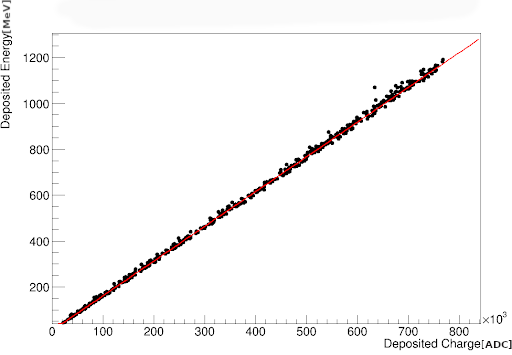
\includegraphics[width = 0.7\textwidth]{figures-chap4/linear_energy_lookup_curve1.png}
%    \captionsetup{type=figure}
%    \captionof{figure}{The linear relationship between deposited charge and energy. Produced from a sample of muons used for calibrating the \textit{Shower Linear Energy tool.}}
%    \label{fig:linear lookup curve}
%\end{center}
\newpage
\begin{figure}[h]
    \centering
    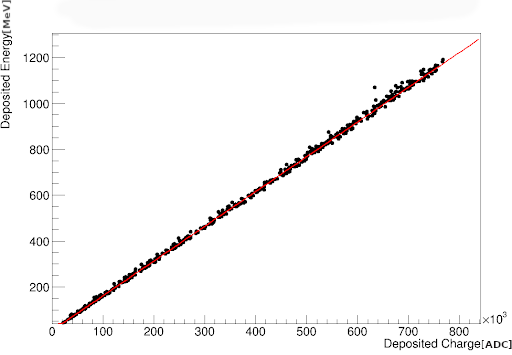
\includegraphics[width = \largefigwidth]{figures-chap4/linear_energy_lookup_curve1.png}
    \caption{The linear relationship between deposited charge and energy. Produced from a sample of muons used for calibrating the \textit{Shower Linear Energy tool.}}
    \label{fig:linear lookup curve}
\end{figure}



To estimate the reconstructed shower energy, the charge found to be associated with a shower would be used to directly read off the associated energy from the linear calibration. A further recombination correction is not required as it has already been accounted for in the charge to energy conversion. The fractional energy resolution of the \textit{Shower Linear Energy tool} is shown in \FigureRef{fig:linear_kGeVelectrons}. 

\subsection{Number of Electrons to Energy}\label{subchap:kGeVToElectrons}
The \textit{Shower Num Electrons Energy tool} was developed to move away from being reliant on in-house calibration curves and instead use the pre-existing calibration available in the \Gls{sbnd} portion of the \Gls{larsoft} framework. This has the advantage of being much more flexible to physics changes. For example a change in the recombination correction could be investigated by changing a single number, whereas, for the \textit{Linear Energy tool}, the calibration curves would have to be regenerated. The number of electrons are found from the \gls{adc} charge and are then directly converted to energy using a \textit{GeVToElectrons} scale factor which is the inverse of the energy required to ionise an argon atom. With this method a correction to account for recombination is still required. A nominal recombination value of 0.64 is used for all hits. 

The nominal recombination value was calculated by simulating electrons with a large (effectively infinite) lifetime and turning off any diffusion effects. The only thing remaining that may impact the collected energy is the recombination effect and therefore taking the ratio between the collected and deposited energy will give a value for the recombination value. For electrons, it was found that the recombination value was fairly constant at a value of 0.64 across a broad range of energies \cite{recombination_0.64}. 



\newpage
\begin{figure}[h]
    \centering
    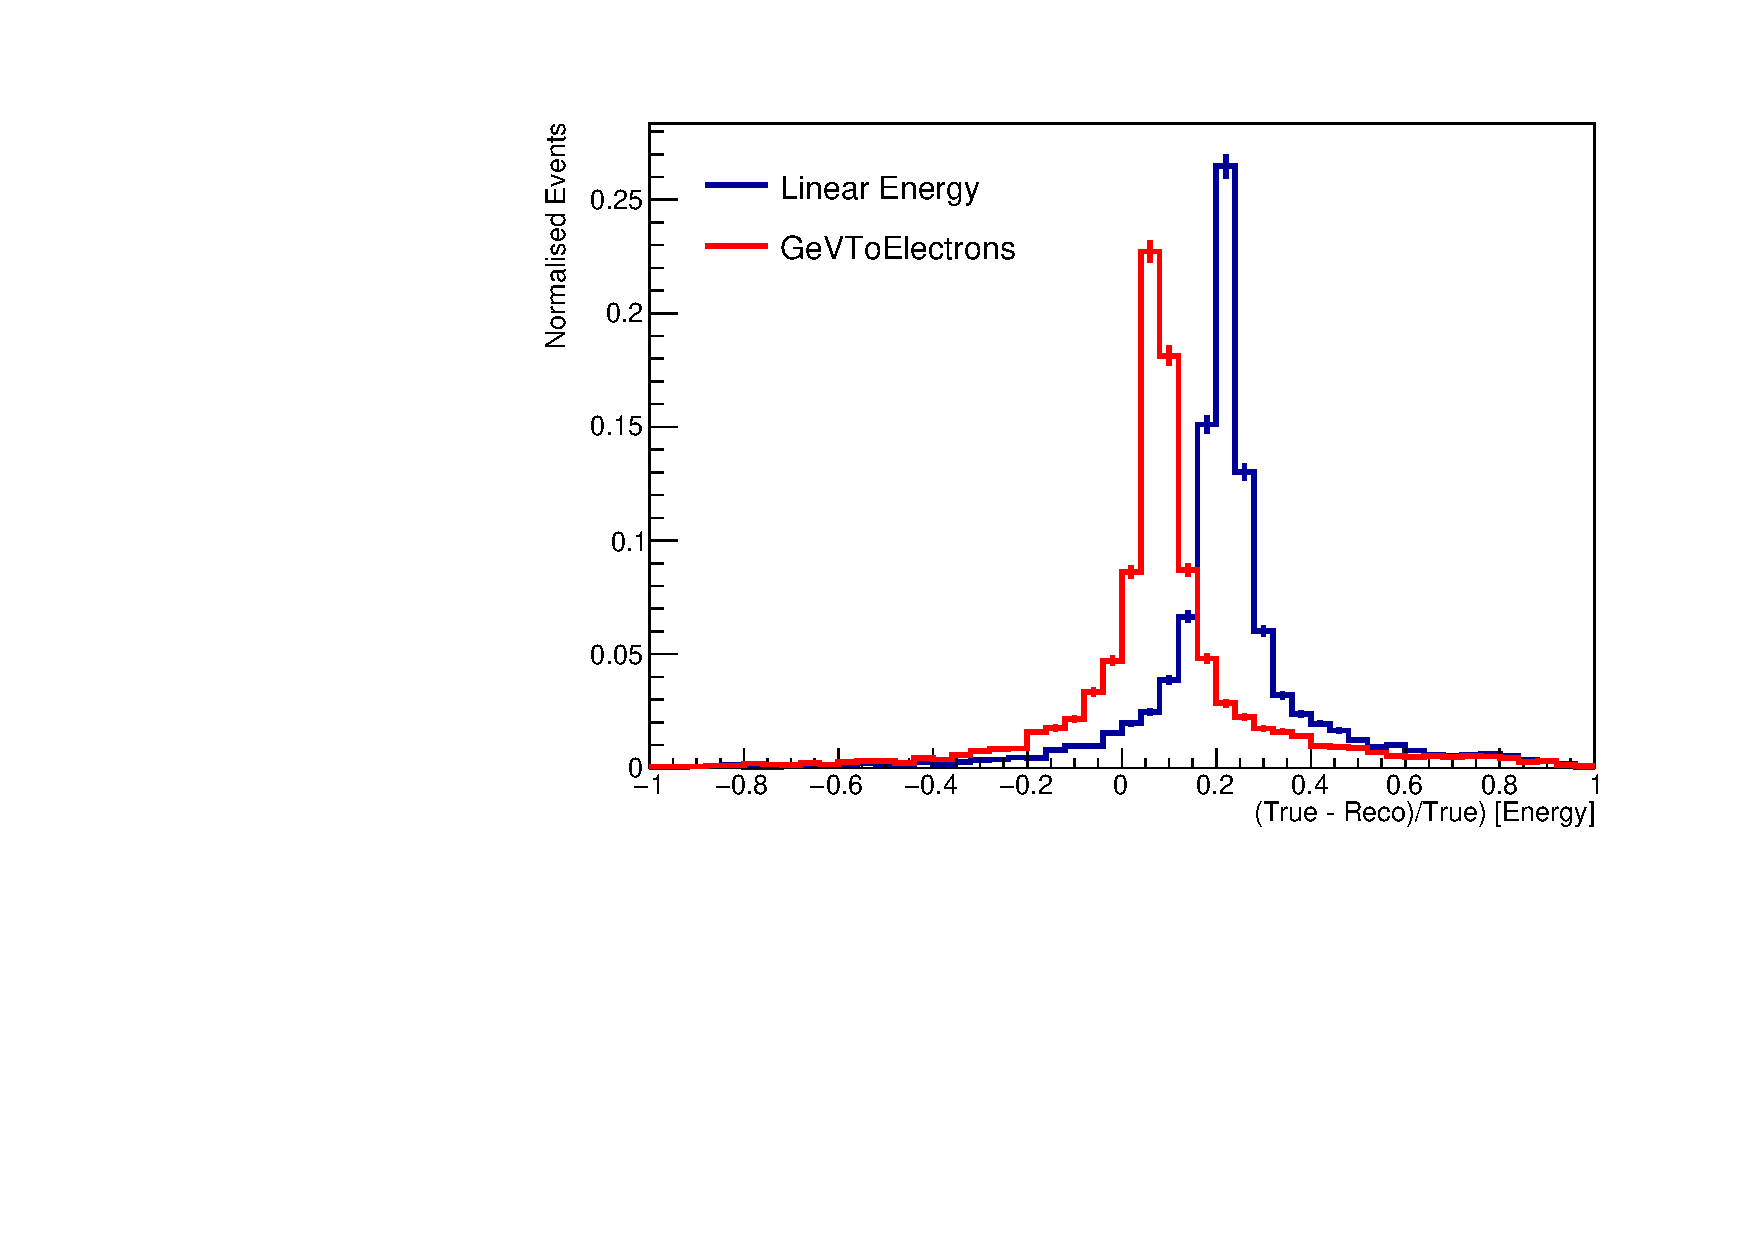
\includegraphics[width = \largefigwidth]{figures-chap4/linear_energy_kGeVElectrons_true_showering.pdf}
    \caption{Comparison of the \textit{Shower Linear Energy Tool} (Blue) and the \textit{Shower Num Electrons Energy Tool} (Red) with the true energy of the showering electrons.}
    \label{fig:linear_kGeVelectrons}
\end{figure}

\begin{comment}

An attempt to correct for the \Gls{sce} can be made with this method by utilising the Modified Box Recombination Model which is given by \begin{equation}\label{eqn:ModBox}
    \frac{dE}{dx} = \frac{\exp{(\frac{\beta}{\rho \mathcal{E}} W_{ion}.\frac{dQ}{dx}}) - \alpha}{\frac{\beta}{\rho \mathcal{E}}}
\end{equation}
where $\frac{dE}{dx}$ is the deposited energy per unit length, $\frac{dQ}{dx}$ is the deposited charge per unit length,  $\mathcal{E}$ is the electric field in the detector, $\rho$ is the density of liquid argon, $W_{ion} = 23.6$ eV which is the energy required to ionise an argon atom, $\alpha = 0.93 \pm 0.02$ and $\beta = 0.212 \pm 0.002$ (kV/cm)(g/cm$^2$)/MeV. The values for parameters $\alpha$ and $\beta$ are results from the \Gls{argoneut} experiment \cite{ArgoNeuT_recombination_paper}. The recombination correction, \textit{R} is given by $\frac{\frac{dQ}{dx}.W_{ion}}{\frac{dE}{dx}}$ and by taking the nominal values of \textit{R} and $\mathcal{E}$ a nominal value for $\frac{dE}{dx}$ is calculated using \EquationRef{eqn:ModBox}. Assuming the nominal value of $\frac{dE}{dx}$ is constant, \textit{R} may be expressed as $R = R(\mathcal{E}$). For each of the hits, their corresponding \Gls{sp} are found and the coordinates of the \Gls{sp} in the detector are determined. Instead of using the nominal value for $\mathcal{E}$, the local value for $\mathcal{E}$ at the position of the \Gls{sp} is used and the corresponding value for \textit{R} is calculated. The method to estimate the reconstructed energy is the same as the case without any \Gls{sce} corrections except the modified value for \textit{R} is used. In the case that a hit has no corresponding \Gls{sp}, the charge weighted centre of the shower is found and the local value of $\mathcal{E}$ at this point is used instead.

\begin{figure}[h]
    \centering
    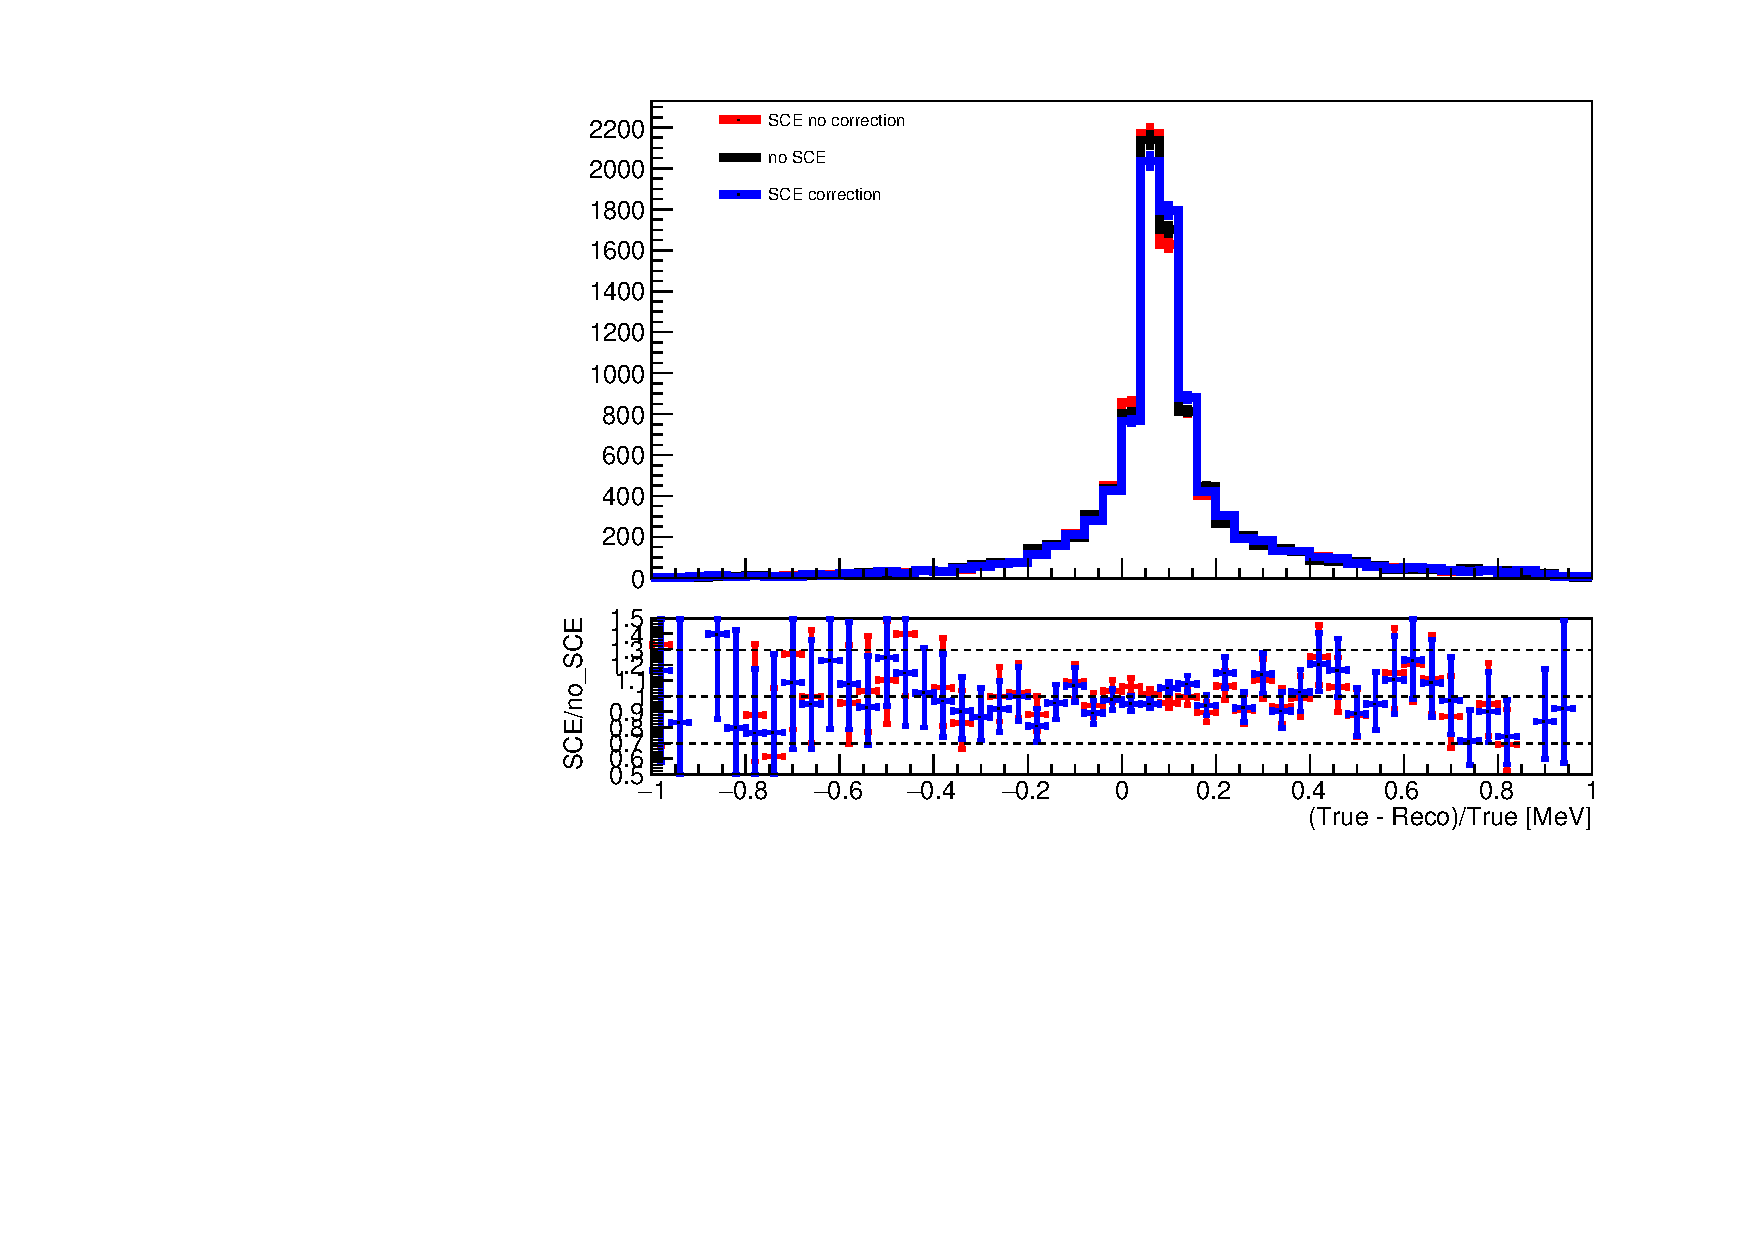
\includegraphics[width = \largefigwidth]{figures-chap4/ratio_plot_oldmethod_trueshoweringparticle.pdf}
    \caption{Caption}
    \label{fig:my_label}
\end{figure}



Shortcoming (don't know how much to put here? don't know if i want to emphasise how bad stuff is..): 
\begin{itemize}
    \item Things revolve around the nominal recomb of 0.64 - not really that realistic. 
    \item Correcting for SCE 'properly' is not straightforward either - using a fixed nominal dE/dx isn't ideal.
\end{itemize}

\end{comment}

\subsection{ESTAR Method}
The \textit{Shower ESTAR Energy tool} combines the ESTAR database provided by the \gls{nist} along with the Modified Box recombination model in an approach that was first used by the \Gls{argoneut} experiment \cite{ArgoNeuT_ESTAR_paper}. The ESTAR database provides the track length of electrons in various materials, including liquid argon, for energies ranging from 0.01 MeV to 1000 MeV \cite{ESTAR_Database}.

$\frac{dE}{dx}$ values may be calculated by dividing the energy by the track length for each entry in the ESTAR database. The deposited charge, \textit{Q}, can then found by using \EquationRef{eqn:ModBox} to find $\frac{dQ}{dx}$ and multiplying by the track length, \textit{dx}. This now allows the collected charge and energy to be related. If $\mathcal{E}$ in \EquationRef{eqn:ModBox} is taken to be a variable, the above process may be repeated whilst iterating over a set values of $\mathcal{E}$. This results in a 3D curve relating both the deposited charge and electric field to energy as is shown in \FigureRef{fig:ESTAR lookup curve}. The energy may then be interpolated from the collected charge and the appropriate electric field. As with the \textit{Linear Energy tool}, a direct correction for recombination isn't needed as it is again accounted for in the lookup curve. 

\begin{figure}[h]
    \centering
    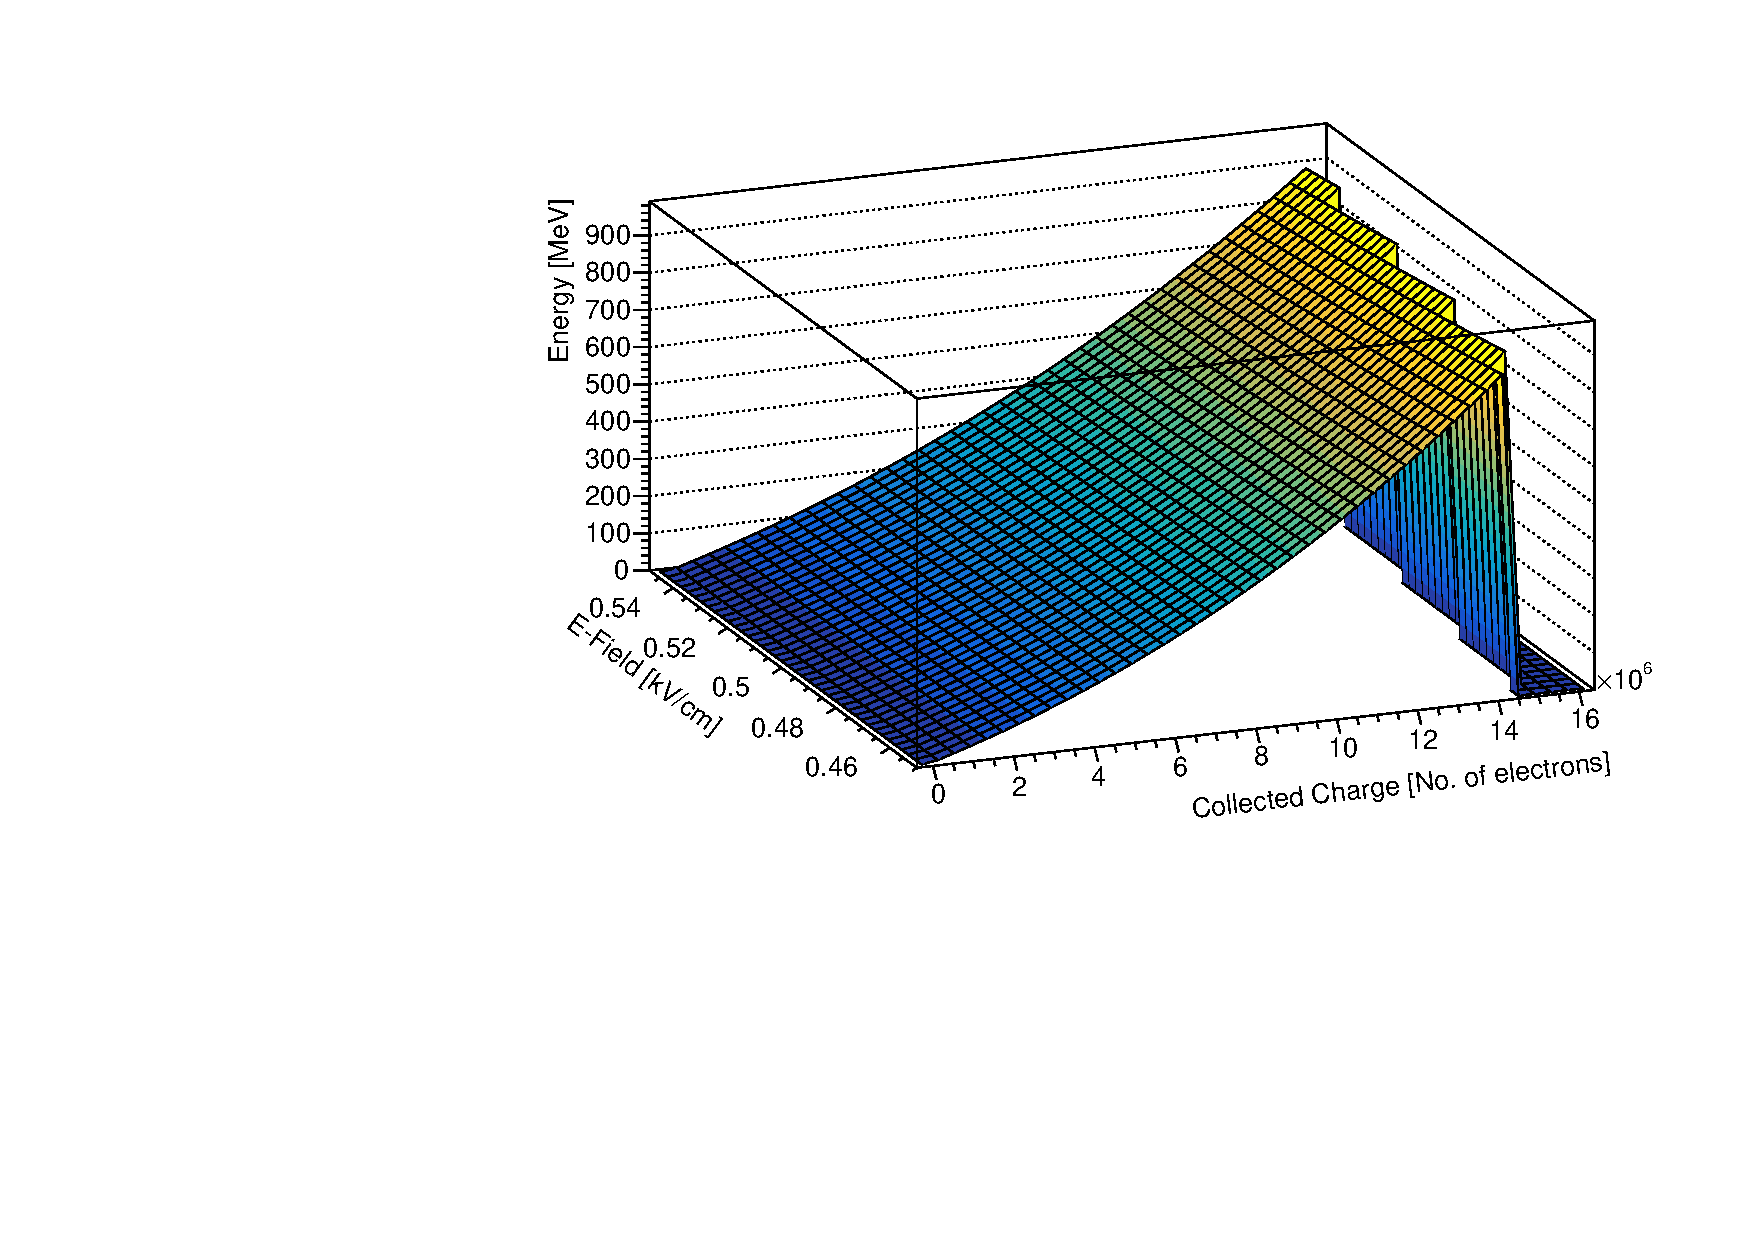
\includegraphics[width = 0.8\textwidth]{figures-chap4/ESTAR_lookup_curve.pdf}
    \caption{ESTAR Lookup Curve}
    \label{fig:ESTAR lookup curve}
\end{figure}

\section{Shower Energy Reconstruction Performance}



To assess the performance of the \textit{Shower ESTAR Energy tool}, the the reconstructed energy of each hit was summed up for all the hits in a shower. This was compared the sum of the true energy of all the hits.


\begin{figure}
    \centering
    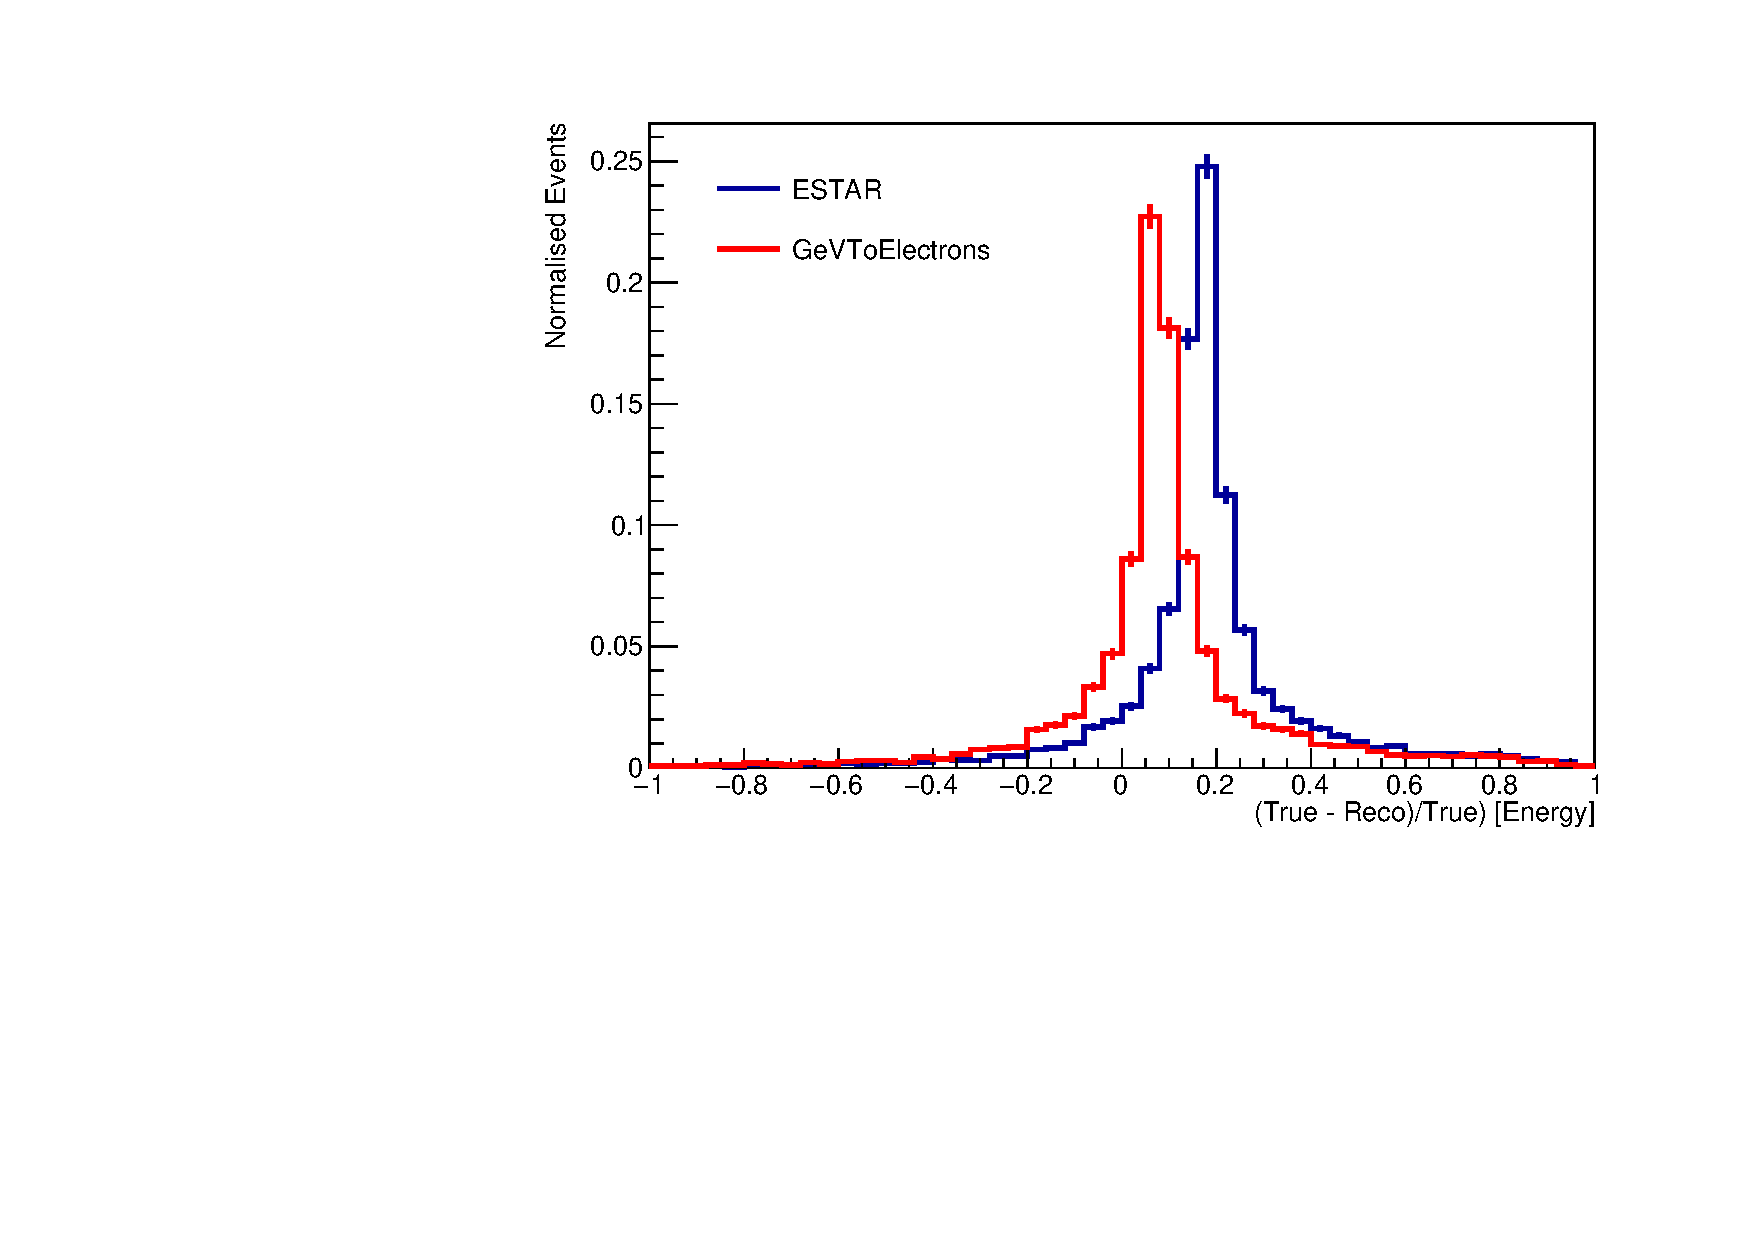
\includegraphics[width = \smallfigwidth]{figures-chap4/ESTAR_kGeVElectrons_true_showering.pdf}
    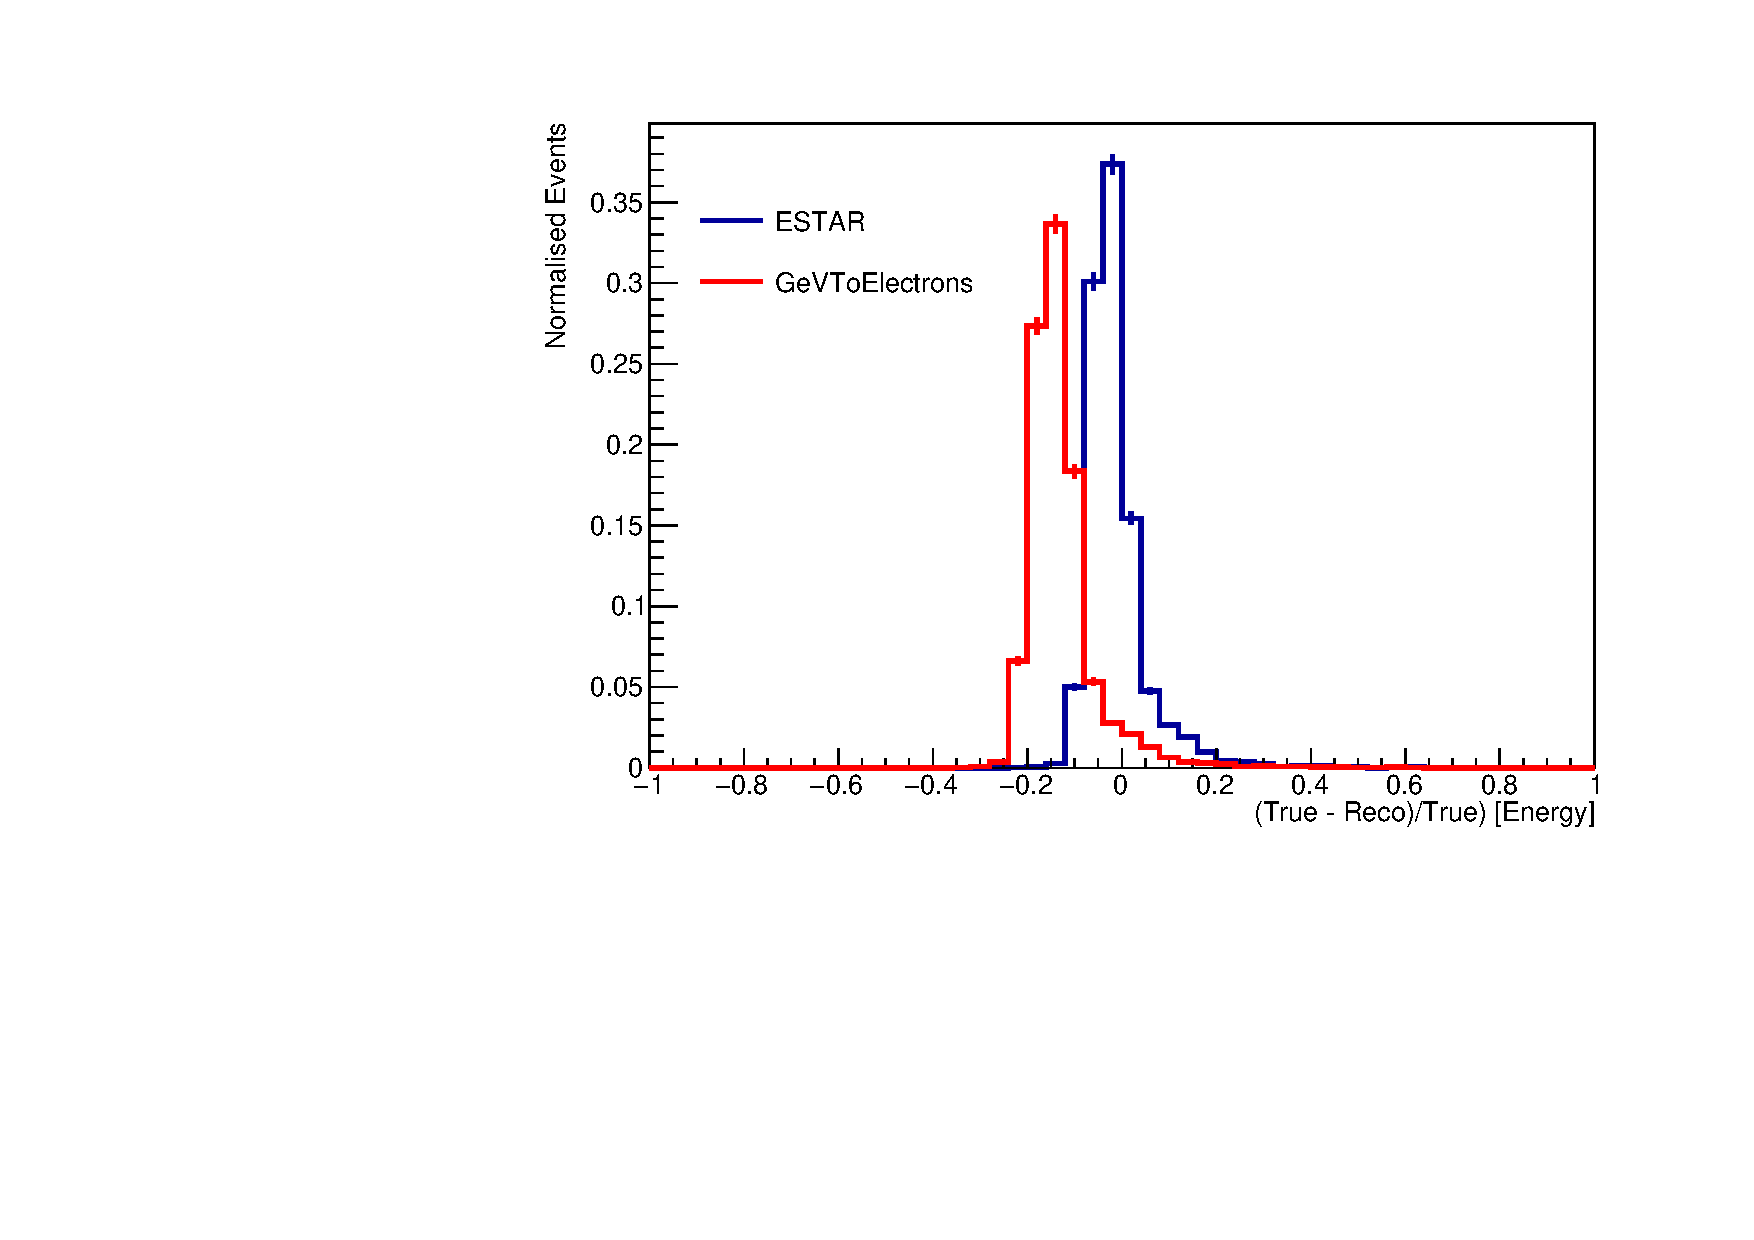
\includegraphics[width = \smallfigwidth]{figures-chap4/ESTAR_kGeVElectrons_true_hit.pdf}
    \caption{The fractional resolution of the \textit{Shower Num Electrons Energy Tool} and \textit{Shower ESTAR Energy Tool} compared with the true energy of the showering electron (left) and the sum of the true energy of all the hits (right). }
    \label{fig:my_label}
\end{figure}

\newpage
Other Validation stuff to do?
\begin{itemize}
    \item Use photon sample?
    \item validate for each individual plane and then best plane?
    \item Look at all showers in an event and compare with total showering energy. 
\end{itemize}


\section{Summary + outstanding issues etc}

Why getting dE/dx is hard (page 17).
Using muons as calibration
Energy bias corrections
https://inspirehep.net/files/f10063871db4836eb6ad935fcf761e7d

Energy Reco - Things to include.

\begin{itemize}
	\item Motivation (why do we care?)
	\item Explain choices - use vertex sample because it helps pandora. Only considering largest shower (most hits) from each event. 
	\item Overview of the very first method that was being used. Use muons to generate lookup curve. Get linear relationship between deposited charge and energy. Plagiarise Dom's thesis on this..  
	\item Change method so we convert the deposited charge to number of electrons and then convert the number of electrons to energy using the appropriate calibration/scale factors. Apply correction for electron lifetime as before and also correct for recombination. Previously recombination correction was 'baked' into the look-up curve. No way to correct for it directly - whenever we would change the \textit{physics} we would need to regenerate the look-up curve. With this method it's possible to tweak the recombination correction directly. 
	\item Not straight forward to calculate the recombination directly - let's use and average value for all showers - explain recombination study. 
	\item Consider SCE - explain what SC is.
	\item How do we account for SCE? Get map of the E-field in the detector (not uniform because of SC). Using the nominal value of the recombination and E-field, calculate a nominal dE/dx (not straightforward to calculate directly) which we assume remains constant. Can now use the Modified Box model to weak the recombination correction by feeding the local E-field (which depends on the location in the detector) back into the modified box model. Finally, find the (charge weighted) centre of the shower using the space points and use the local E-field at this point to calculate the recombination factor at this location. 
	\item No reason we can't do a per-hit analysis. Redo everything as before for each individual hit and then sum to get the energy of the shower. Should give better results since the recombination correction is more accurate now. 
	\item We have the ability to attempt to correct for the SCE as mentioned, but are limited by not knowing the dE/dx. So correcting the SCE without this caveat becomes tricky.. Try a new approach developed by ArgoNeuT - use the ESTAR database. The ESTAR database gives us the stopping power of (dE/dx) of electrons in various materials (including lAr) in a range of energies and is based partly from data. Combining this with the modified box recombination model, we can again create a lookup curve of energy vs deposited charge with the recombination correction baked in. Since the modified box model depends on the E-Field, we can treat this as a variable and create a 3D lookup curve of energy vs E-Field vs deposited charge which will allow us to correct for SC. 
	\item \textit{True} energy debacle.. We have the true energy of the showering particle and the true energy of all the hits in a given shower. Originally we used the true energy of the showering particle for comparison (in hindsight this seems like a stupid idea..) and the kGeVtoElectrons method clearly outperformed ESTAR. Swapping to the true hit energies, ESTAR does better. What was happening (i think) is that kGeVToElectrons over estimates the hit energies, so when comparing with the true showering particle this method give a better result because we're papering over the cracks due to the pattern recognition and hit inefficiencies. ESATR method gives a better result for individual hit energies so highlights the failing of the patter rec and hit inefficiencies when comparing with the showering particle. 
	\item Why some results are shit.. Pandora pattern recognition (clustering) is far from perfect - can use Pandora in cheating mode to overcome this. There are hit inefficiencies i.e. hit reconstruction isn't perfect - haven't ever \textit{cheated} this, dunno if it's an option. The actual impact from SC is pretty minimal but it also impacts Pandora's pattern recognition. This can a have a big impact - what Pandora initially recognised as one big shower may be interpreted as 2+ smaller showers after applying SC (and vice-versa). Also, an object classified as a shower may instead be classified as a track after applying SC. Since we're only considering the largest shower for each event, this effects mean SC can appear to have a impact. 
\end{itemize}

  %\chapter{Sterile Neutrino Oscillation Inputs Within SBN}
\label{chap:osc_inputs}


\begin{figure}[!h]
    \centering
    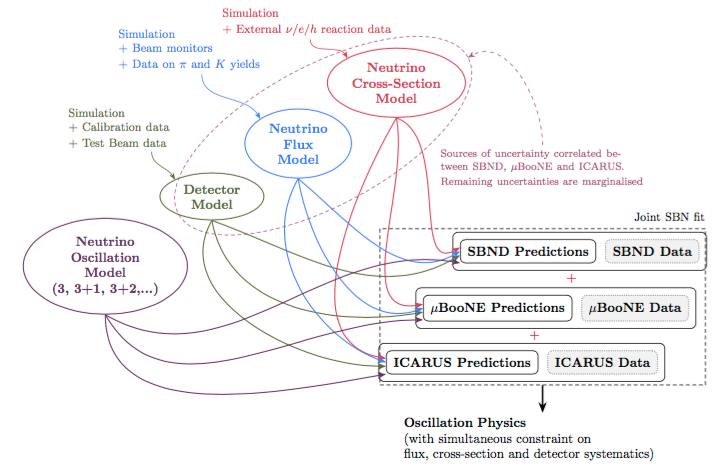
\includegraphics[width = \largefigwidth]{figures-chap5/valor_analysis.png}
    \caption{Overview of the SBN oscillation analysis paradigm. A given model for the neutrino oscillation, detector, neutrino flux and neutrino cross-section are combined with the appropriate data to give the prediction for the respective detector. Individual detector predictions may be combined to give an overall \gls{sbn} prediction. }
    \label{fig:analysis_paradigm}
\end{figure}

\section{Event Production}


\subsection{\texorpdfstring{\numu}{numu}}
\subsection{\texorpdfstring{\nue}{nue}}
The $\nue $ production followed the same steps described in section \ref{S:MCSamples:NumuProd}, however, in addition to generating an intrinsic $\nue$ sample, an oscillated $\numu \rightarrow \nue$ sample, a dirt sample and a cosmic sample were also produced. The oscillated sample is used to mimic the $\nue$ appearance signal whereas the dirt and cosmic samples are backgrounds. The other major background associated with a $\nue$ analysis involves $\numu$. A dedicated sample was not produced to emulate this, but instead the events from the $\numu$ production were also ran through the $\nue$ selection as mentioned in section \ref{S:NuESelection}. Table \ref{T:nue_production} outlines the number of events produced for each sample for each detector. The dirt events were produced with an additional filter at the generation stage which discarded any events where a shower above 10 MeV in the active volume was not present. This filter was used in order to remove any delta rays. Only about 1\% of dirt events would pass this filter so the number of dirt events used in the $\nue$ selection was $\sim$100,000. 


\begin{table}[h!]
\begin{tabular}{c cc}
Sample        & \begin{tabular}[c]{@{}c@{}}Events Produced\end{tabular} \\ \hline

Intrinsic $\nue$ & $\sim$1,000,000      \\
Oscillated $\nu$ & $\sim$1,000,000      \\
$\numu$          & {See $\nu_{\mu}$ sample}  \\
Dirt          & $\sim$10,000,000        \\
Cosmic\_Dirt  & $\sim$100,000             

\end{tabular}
\caption{The number of events initially produced for each sample in each of the three SBN detectors as part of the $\nue$ analysis.}
\end{table}\label{T:nue_production}


\section{\texorpdfstring{$\nu_\mu$ and $\nu_e$ Selections}{numu and nue Selections}}
Link in with Energy Reco. section

\section{Reaction Modes}
\subsection{Fine}

% Fine reaction modes
\begin{table}[t!]
  \renewcommand{\arraystretch}{1.6}
  \begin{tabular}{>{\centering\arraybackslash}m{4cm} 
                  >{\centering\arraybackslash}m{4cm}
                  >{\centering\arraybackslash}m{4cm}}
  
    \toprule
    \multicolumn{3}{c}{\textit{Fine Reaction Modes}} \\
    $\numu$, $\numubar$ & $\nue$, $\nuebar$ & $\numu \rightarrow \nue, \numubar \rightarrow \nuebar$ \\
    \midrule
    CC QE                      & CC QE                     & CC QE\\
    NC~Elastic                 & NC~Elastic                & CC MEC\\ 
    CC, NC MEC                 & CC, NC MEC                & CC 1$\pi^{\pm}$ \\  
    CC, NC 1$\pi^{\pm}$        & CC, NC 1$\pi^{\pm}$       & CC 1$\pi^{0}$ \\   
    CC, NC 1$\pi^{0}$          & CC, NC 1$\pi^{0}$         & CC 2$\pi^{\pm}$ \\   
    CC, NC 2$\pi^{\pm}$        & CC, NC 2$\pi^{\pm}$       & CC 2$\pi^{0}$i \\   
    CC, NC 2$\pi^{0}$          & CC, NC 2$\pi^{0}$         & CC Coh \\   
    CC, NC $\pi^{\pm}\pi^{0}$  & CC, NC $\pi^{\pm}\pi^{0}$ & Elastic Scattering \\   
    CC, NC Coh                 & CC, NC Coh                & CC Other \\  
    CC, NC Elastic Scattering  & CC+NC Elastic Scattering  \\  
    NC 1$\gamma$               & NC 1$\gamma$              \\  
    CC, NC Other               & CC, NC Other              \\  
    \hdashline
    \multicolumn{3}{c}{\textit{Cosmic \& Dirt}} \\
    \bottomrule

  \end{tabular}
  \caption[Fine Reaction Modes]{The complete list of reaction modes considered in an \gls{sbn} analysis.}
  \label{table:fine_reac_modes}
\end{table}




\subsection{Coarse}
% Coarse reaction modes
\begin{table}[t!]
  \begin{tabular}{>{\centering\arraybackslash}m{4cm} 
    >{\centering\arraybackslash}m{4cm}}
  
    \toprule
    \multicolumn{2}{c}{\textit{Coarse Reaction Modes}} \\
    $\numu$, $\numubar$ & $\nue$, $\nuebar$ \\
    \midrule
    $\numu$ CC QE          & \nue CC QE          \\ 
    $\numu$ CC MEC         & \nue CC MEC         \\ 
    $\numu$ CC 1$\pi$      & \nue CC 1$\pi$      \\ 
    $\numu$ CC 2$\pi$      & \nue CC 2$\pi$      \\ 
    $\numu$ CC Other       & \nue CC Other       \\ 
    $\numubar$ CC          & \nuebar CC          \\
    $\nue$ \& $\nuebar$ CC & \numu CC            \\
    NC                     & \numubar CC         \\
    \textit{Cosmic}        & Oscillated \nue CC  \\
    \textit{Dirt}          & NC 0\pi             \\
                           & NC Other            \\
                           & \textit{Cosmic}     \\
                           & \textit{Dirt}       \\
    \bottomrule

  \end{tabular}
  \caption[Coarse Reaction Modes]{The \textit{coarse} reaction modes used for both the \numu and \nue channels. These are broader definition of the reaction modes where one or more of the \textit{fine} reaction modes listed in \TableRef{table:fine_reac_modes} would come under the umbrella of a given coarse reaction mode.}
  \label{table:coarse_reac_modes}
\end{table}


\section{Flux Systematics}

\begin{table}[!h]
  \renewcommand{\arraystretch}{1.4}    
  \begin{tabular}{p{2.5cm} p{9.2cm} p{1.2cm} p{1.2cm}}
    \toprule
    \multirow{2}{*}{Parameter} & \multirow{2}{*}{Description} & \multicolumn{2}{c}{Uncertainty} \\
    && \multicolumn{1}{c}{Be} & \multicolumn{1}{c}{Al} \\
    \midrule

    $f_{\sigma_{INEL}^{N}}$   & Secondary inelastic nucleon cross-section in the target (Be) and horn (Al) & $\pm 5 \%$ & $\pm 10 \%$\\
                            
    $f_{\sigma_{QE}^{N}}$     & Secondary quasi-elastic nucleon cross-section in the target (Be) and horn (Al) & $\pm 20 \%$ & $\pm 45 \%$\\
                            
    $f_{\sigma_{TOT}^{N}}$    & Secondary total nucleon cross-section in the target (Be) and horn (Al) & $\pm 15 \%$ & $\pm 25 \%$\\

    $f_{\sigma_{INEL}^{\pi}}$ & Secondary inelastic pion cross-section in the target (Be) and horn (Al) & $\pm 10 \% $ & $\pm 20 \% $\\
                          
    $f_{\sigma_{QE}^{\pi}}$   & Secondary quasi-elastic pion cross-section in the target (Be) and horn (Al) & $\pm 11.2 \% $ & $\pm 25.9 \% $\\
                          
    $f_{\sigma_{TOT}^{\pi}}$  & Secondary total pion cross-section in the target (Be) and horn (Al) & $\pm 11.9 \%$ & $\pm 28.7 \%$\\
    \bottomrule
  \end{tabular}
  \caption[Hadronic secondary interaction flux systematic parameters]{The systematic uncertainties associated with secondary hadron interaction cross-sections in both the horn (Aluminium) and the target (Berylium) \cite{SBN_Proposal}}.
  \label{}
\end{table}


\begin{table}[!h]
  \renewcommand{\arraystretch}{1.4}    
  \begin{tabular}{p{2.5cm} p{10cm} p{2cm}}

    \toprule
    Parameter & Description & Uncertainty \\ 
    \midrule

    $f_{SkinEffect}$  & Depth that the current penetrates the horn conductor & $<18 \%$\\

    $f_{HornCurrent}$ & Current running in the horn conductor & $\pm 0.6 \%$\\
    \bottomrule

  \end{tabular}
  \caption[Optical, beam focusing flux systematic parameters]{Optical systematic flux uncertainties associated with the current in the horn\cite{BNB_flux}.}
  \label{}
\end{table}

\begin{table}[!h]
  \renewcommand{\arraystretch}{1.4}    
  \begin{tabular}{p{2cm} p{6.0cm} p{1.2cm} p{1.2cm} p{1.2cm} p{1.2cm}}
    \toprule
    \multirow{2}{*}{Parameter} & \multirow{2}{*}{Description} & \multicolumn{4}{c}{Uncertainty} \\
    && \multicolumn{1}{c}{$\nu_{\mu}$} & \multicolumn{1}{c}{$\bar{\nu}_{\mu}$} & \multicolumn{1}{c}{$\nu_{e}$} & \multicolumn{1}{c}{$\bar{\nu}_{e}$} \\
    \midrule

    $f_{\pi^{+}}$ & $\nu$ production mechanism: $\pi^{+}$ & $ \pm 11.7 \%$ & $ \pm 1.0 \%$ & $ \pm 10.7 \%$ & $ \pm 0.03 \%$ \\

    $f_{\pi^{-}}$ & $\nu$ production mechanism: $\pi^{-}$ & $ \pm 0.0 \%$ & $ \pm 11.6 \%$ & $ \pm 0.0 \%$ & $ \pm 3.0 \%$ \\

    $f_{K^{+}}$   & $\nu$ production mechanism: $K^{+}$ & $ \pm 0.2 \%$ & $ \pm 0.1 \%$ & $ \pm 2.0 \%$ & $ \pm 0.1 \%$ \\
                  
    $f_{K^{-}}$   & $\nu$ production mechanism: $K^{-}$ & $ \pm 0.0 \%$ & $ \pm 0.4 \%$ & $ \pm 0.0 \%$ & $ \pm 3.0 \%$ \\
                  
    $f_{K^{0}}$   & $\nu$ production mechanism: $K^{0}$ & $ \pm 0.0 \%$ & $ \pm 0.3 \%$ & $ \pm 2.3 \%$ & $ \pm 21.4 \%$ \\

    \bottomrule
  \end{tabular}
  \caption[Hadron production flux systematic parameters]{Hadron production systematic flux uncertainties \cite{BNB_flux_TN}.}
  \label{}
\end{table}


\section{Interaction Systematics}

\begin{table}[h!]
    \renewcommand{\arraystretch}{1.4}
    \begin{tabular}{p{1.8cm} p{10cm}>{\centering\arraybackslash}p{ 2.2cm}}
        \toprule
         Parameter & Description & $\delta P / P$ \\
        \midrule
         $f_{M_{A}^{CCQE}}$  & Axial mass for CC quasi-elastic & -15\% +25\% \\
         
         $f_{M_{A}^{CCRes}}$ & Axial mass for CC resonance neutrino production & $\pm 20\%$ \\
         
         $f_{M_{A}^{NCRes}}$ & Axial mass for NC resonance neutrino production & $\pm 20\%$ \\
         
         $f_{NC}$              & Additional error on NC/CC ratio & $\pm 25\%$ \\
         
         $f_{nR_{\nu n}^{CC1\pi}}$ & Non-resonance bkg normalisation in $\nu n$ CC1$\pi$ reactions & $\pm 50\%$ \\
         
         $f_{nR_{\nu p}^{CC1\pi}}$ & Non-resonance bkg normalisation in $\nu p$ CC1$\pi$ reactions & $\pm 50\%$ \\
         
         $f_{nR_{\nu n}^{CC2\pi}}$ & Non-resonance bkg normalisation in $\nu n$ CC2$\pi$ reactions & $\pm 50\%$ \\
         
         $f_{nR_{\nu p}^{CC2\pi}}$ & Non-resonance bkg normalisation in $\nu p$ CC2$\pi$ reactions & $\pm 50\%$ \\
         
         $f_{nR_{\bar{\nu} n}^{CC1\pi}}$ & Non-resonance bkg normalisation in $\bar{\nu} n$ CC1$\pi$ reactions & $\pm 50\%$ \\
         
         $f_{nR_{\bar{\nu} p}^{CC1\pi}}$ & Non-resonance bkg normalisation in $\bar{\nu} p$ CC1$\pi$ reactions & $\pm 50\%$ \\
         
         $f_{nR_{\bar{\nu} n}^{CC2\pi}}$ & Non-resonance bkg normalisation in $\bar{\nu} n$ CC2$\pi$ reactions & $\pm 50\%$ \\
         
         $f_{nR_{\bar{\nu} p}^{CC2\pi}}$ & Non-resonance bkg normalisation in $\bar{\nu} p$ CC2$\pi$ reactions & $\pm 50\%$ \\
        
         $f_{nR_{\nu n}^{NC1\pi}}$ & Non-resonance bkg normalisation in $\nu n$ NC1$\pi$ reactions & $\pm 50\%$ \\
         
         $f_{nR_{\nu p}^{NC1\pi}}$ & Non-resonance bkg normalisation in $\nu p$ NC1$\pi$ reactions & $\pm 50\%$ \\
         
         $f_{nR_{\nu n}^{NC2\pi}}$ & Non-resonance bkg normalisation in $\nu n$ NC2$\pi$ reactions & $\pm 50\%$ \\
         
         $f_{nR_{\nu p}^{NC2\pi}}$ & Non-resonance bkg normalisation in $\nu p$ NC2$\pi$ reactions & $\pm 50\%$ \\
         
         $f_{nR_{\bar{\nu} n}^{NC1\pi}}$ & Non-resonance bkg normalisation in $\bar{\nu} n$ NC1$\pi$ reactions & $\pm 50\%$ \\
         
         $f_{nR_{\bar{\nu} p}^{NC1\pi}}$ & Non-resonance bkg normalisation in $\bar{\nu} p$ NC1$\pi$ reactions & $\pm 50\%$ \\
         
         $f_{nR_{\bar{\nu} n}^{NC2\pi}}$ & Non-resonance bkg normalisation in $\bar{\nu} n$ NC2$\pi$ reactions & $\pm 50\%$ \\
         
         $f_{nR_{\bar{\nu} p}^{NC2\pi}}$ & Non-resonance bkg normalisation in $\bar{\nu} p$ NC2$\pi$ reactions & $\pm 50\%$ \\
        
        \bottomrule
        
    \end{tabular}
    \caption[SBN proposal interaction cross-section systematic parameters]{GENIE interaction cross-section systematics considered in \gls{sbn} as part of the \textit{proposal} set of systematics. \cite{GENIE_manual}.}
    \label{}
\end{table}


\begin{table}[h!]
    \renewcommand{\arraystretch}{1.4}
    \begin{tabular}{p{1.8cm} p{10cm}>{\centering\arraybackslash}p{ 2.2cm}}
        \toprule
         Parameter & Description & $\delta P / P$ \\
        \midrule
         $f_{M_{A}^{NCEl}}$  & Axial mass for NC elastic & $\pm 25\%$ \\
         
         $f_{\eta^{NCEl}}$    & Strange axial form factor for NC elastic & $\pm 30\%$ \\
        
         %$f_{2p2h}$          & Normalisation uncertainty for 2p2h interactions & $\pm 100\%$ \\
         
         $f_{M_{V}^{CCRes}}$ & Vector mass for CC resonance neutrino production & $\pm 10\%$ \\
         
         $f_{M_{V}^{NCRes}}$ & Vector mass for NC resonance neutrino production & $\pm 10\%$ \\
         
         $f_{A_{HT}}$          & Higher-twist parameter A for NC and CC DIS events & $\pm 25\%$ \\
         
         $f_{B_{HT}}$          & Higher-twist parameter B for NC and CC DIS events & $\pm 25\%$ \\
         
         $f_{C_{v1u}}$         & Valence p.d.f. correction factor $C_{v1u}$ for DIS events & $\pm 30\%$ \\
         
         $f_{C_{v2u}}$         & Valence p.d.f. correction factor $C_{v2u}$ for DIS events & $\pm 40\%$ \\
         
         $f_{M_{A}^{Coh}}$     & Axial mass for NC and CC coherent pion production & $ \pm 50 \%$ \\
         
         $f_{R_{0}^{Coh}}$     & Nuclear size parameter controlling $\pi$ absorption & $\pm 20 \%$ \\
        
        $f_{\Delta\rightarrow N\gamma}$   & Branching ratio for $\Delta$ radiative decay & $\pm 50 \%$ \\
        
        \bottomrule
        
    \end{tabular}
    \caption[Modern interaction cross-section systematic parameters]{GENIE interaction cross-section systematics considered in \gls{sbn} as part of the \textit{modern} set of systematics \cite{GENIE_manual}.}

    \label{}
\end{table}


\begin{table}[!h]
    \renewcommand{\arraystretch}{1.4}
    \begin{tabular}{p{1.8cm} p{11.4cm} p{1.2cm}}
        \toprule
         Parameter & Description & $\delta P / P$ \\
        \midrule
        
         $f_{\lambda_{\pi}}$   & Intranuclear mean free path for pions & $ \pm 20 \% $ \\
        
         $f_{R^{CEx}_{\pi}}$    & Intranuclear charge exchange rescattering fraction for pions & $ \pm 50 \% $ \\
        
         $f_{R^{Inel}_{\pi}}$   & Intranuclear inelastic rescattering fraction for pions & $ \pm 40 \% $ \\
        
         $f_{R^{\pi}_{\pi}}$    & Intranuclear pion-production rescattering fraction for pions & $ \pm 20 \% $ \\
        
         $f_{R^{Abs}_{\pi}}$    & Intranuclear absorption fraction for pions & $ \pm 20 \% $ \\
        
         $f_{\lambda_{N}}$     & Intranuclear mean free path for nucleons & $ \pm 20 \% $ \\
        
         $f_{R^{CEx}_{N}}$      & Intranuclear charge exchange rescattering fraction for nucleons & $ \pm 50 \%$ \\
        
         $f_{R^{Inel}_{N}}$     & Intranuclear inelastic rescattering fraction for nucleons & $ \pm 40 \% $ \\
        
         $f_{R^{\pi}_{N}}$      & Intranuclear pion-production rescattering fraction for nucleons & $ \pm 20 \% $ \\
        
         $f_{R^{Abs}_{N}}$      & Intranuclear absorption fraction for nucleons & $ \pm 20 \% $ \\

        \bottomrule
    \end{tabular}
    \caption[Intranuclear hadron transport systematic parameters]{\cite{GENIE_manual}}
    \label{}
\end{table}


\section{Other Systematics}
MEC, POT, Detector, Energy scale - maybe put some of these in above sections.
\section{Other Analysis Choices}
All the stuff that was 'agreed' between fitters - Baseline Approximation, Binning, Spectra energy range etc.

\subsection{Baseline}
As is shown in \EquationRef{eqn:sterile_osc_prob}, the baseline is one of the components that drives the oscillation probability. For long baseline experiments, it's not uncommon for fitting frameworks to simply use some average value for the baseline since factors such as the interaction point in the detector or the position at which a particle decays into a neutrino would only change the average baseline for the experiment by a negligible amount. However, for short baseline experiments such as \gls{sbn}, these factors may change the baseline significantly. 

In an attempt to minimise computing resources, the true baseline was not initially used, but instead several approximations to the baseline were tried. To begin with, the average baseline of each \gls{sbn} detector was used for all neutrino energies. This was calculated from the true baseline distribution of \numu events in each detector which are shown in \FigureRef{fig:numu_baseline}. Secondly, a 4-knot spline (named spline V1) for each detector was defined in order to try and better approximate the baseline. This method was improved upon by producing a spline for each of the true energy bins (named spline V2) which are defined in \SectionRef{sec:binning}. In order to establish the impact of any baseline approximations on the oscillation probability, the oscillation probability was plotted as a function of true neutrino energy with the oscillation parameters $sin^22\theta_{\mu\mu} = 0.01$ and $\Delta m^2_{41} = 50$ eV$^2$. This oscillation point was chosen to ensure that a region where rapid oscillation occur was being investigated, which would highlight the effect of any baseline choices. The oscillation probabilities as a function of energy are shown in \FigureRef{fig:baseline_osc_probability} for the four different baselines described. It was eventually decided that any approximation would be insufficient and that the true baseline should be used. 

The studies of the baseline approximations were done in the context of the \numu disappearance channel. For the \nue channels, different approximations should be applied, since the true baseline distribution is not the same as for \numu. In principal, within the \nue sample, different approximations should be applied to the different sub-samples since the baseline distribution is not the same for all the sub-samples. This was never done since it was decided that the true baseline should be used. Each individual sample used to construct the overall \nue event sample, has it's own baseline distribution due to the particles which contribute to each sample decaying at different points along the beamline. The baseline distribution for the intrinsic \nue, oscillated \nue and the overall \nue sample from combining all the sub-samples together is shown in \FigureRef{fig:nue_baseline_dist} for each of the \gls{sbn} detectors. It should be noted that the baseline distributions for oscillated \nue sample from \FigureRef{fig:nue_baseline_dist} and the \numu sample from \FigureRef{fig:numu_baseline} are comparable. This is due to the initial parameters describing the oscillated sample being the same as for the \numu sample. The only difference being the neutrino oscillations from \numu to \nue which isn't something that affects the baseline.

\begin{figure}[!h]
    \centering
    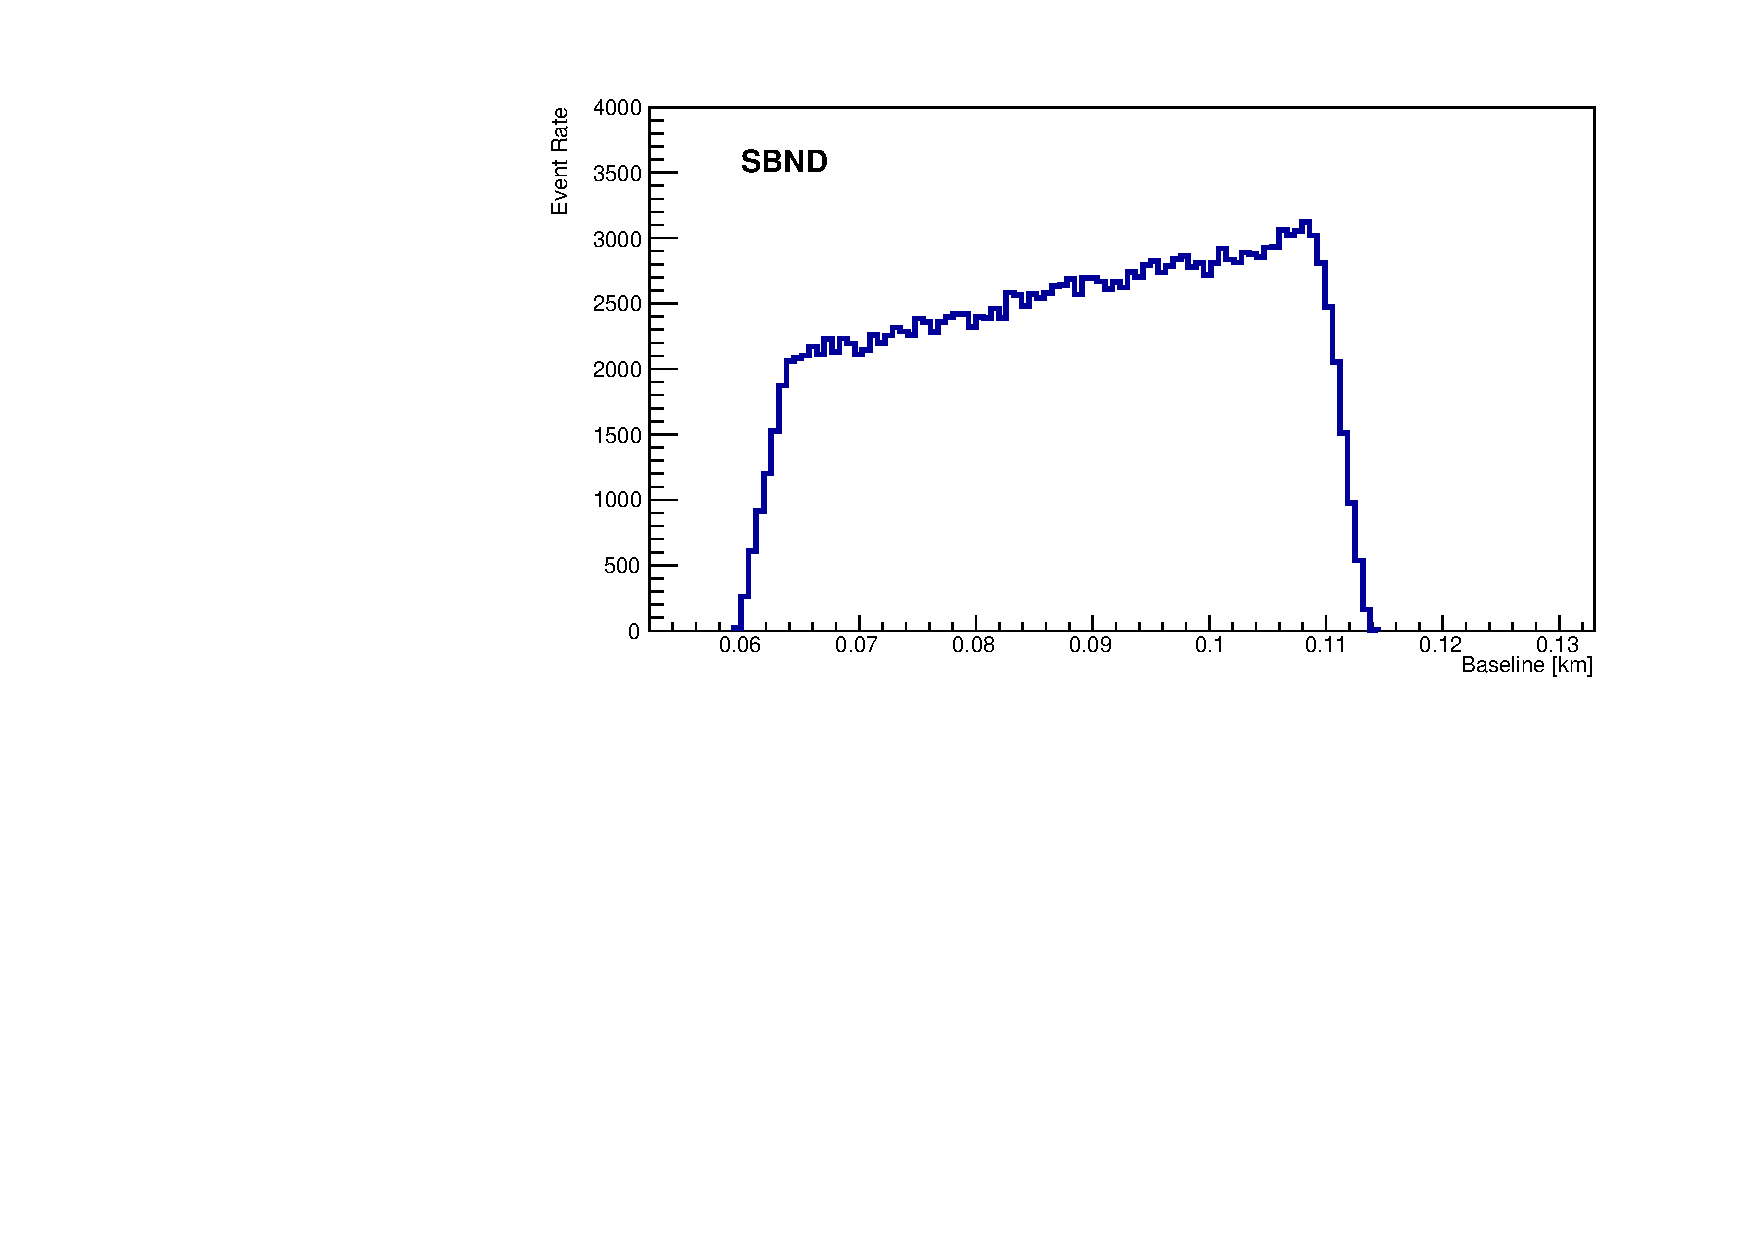
\includegraphics[width = 0.32\textwidth]{figures-chap5/SBND_numu.pdf}
    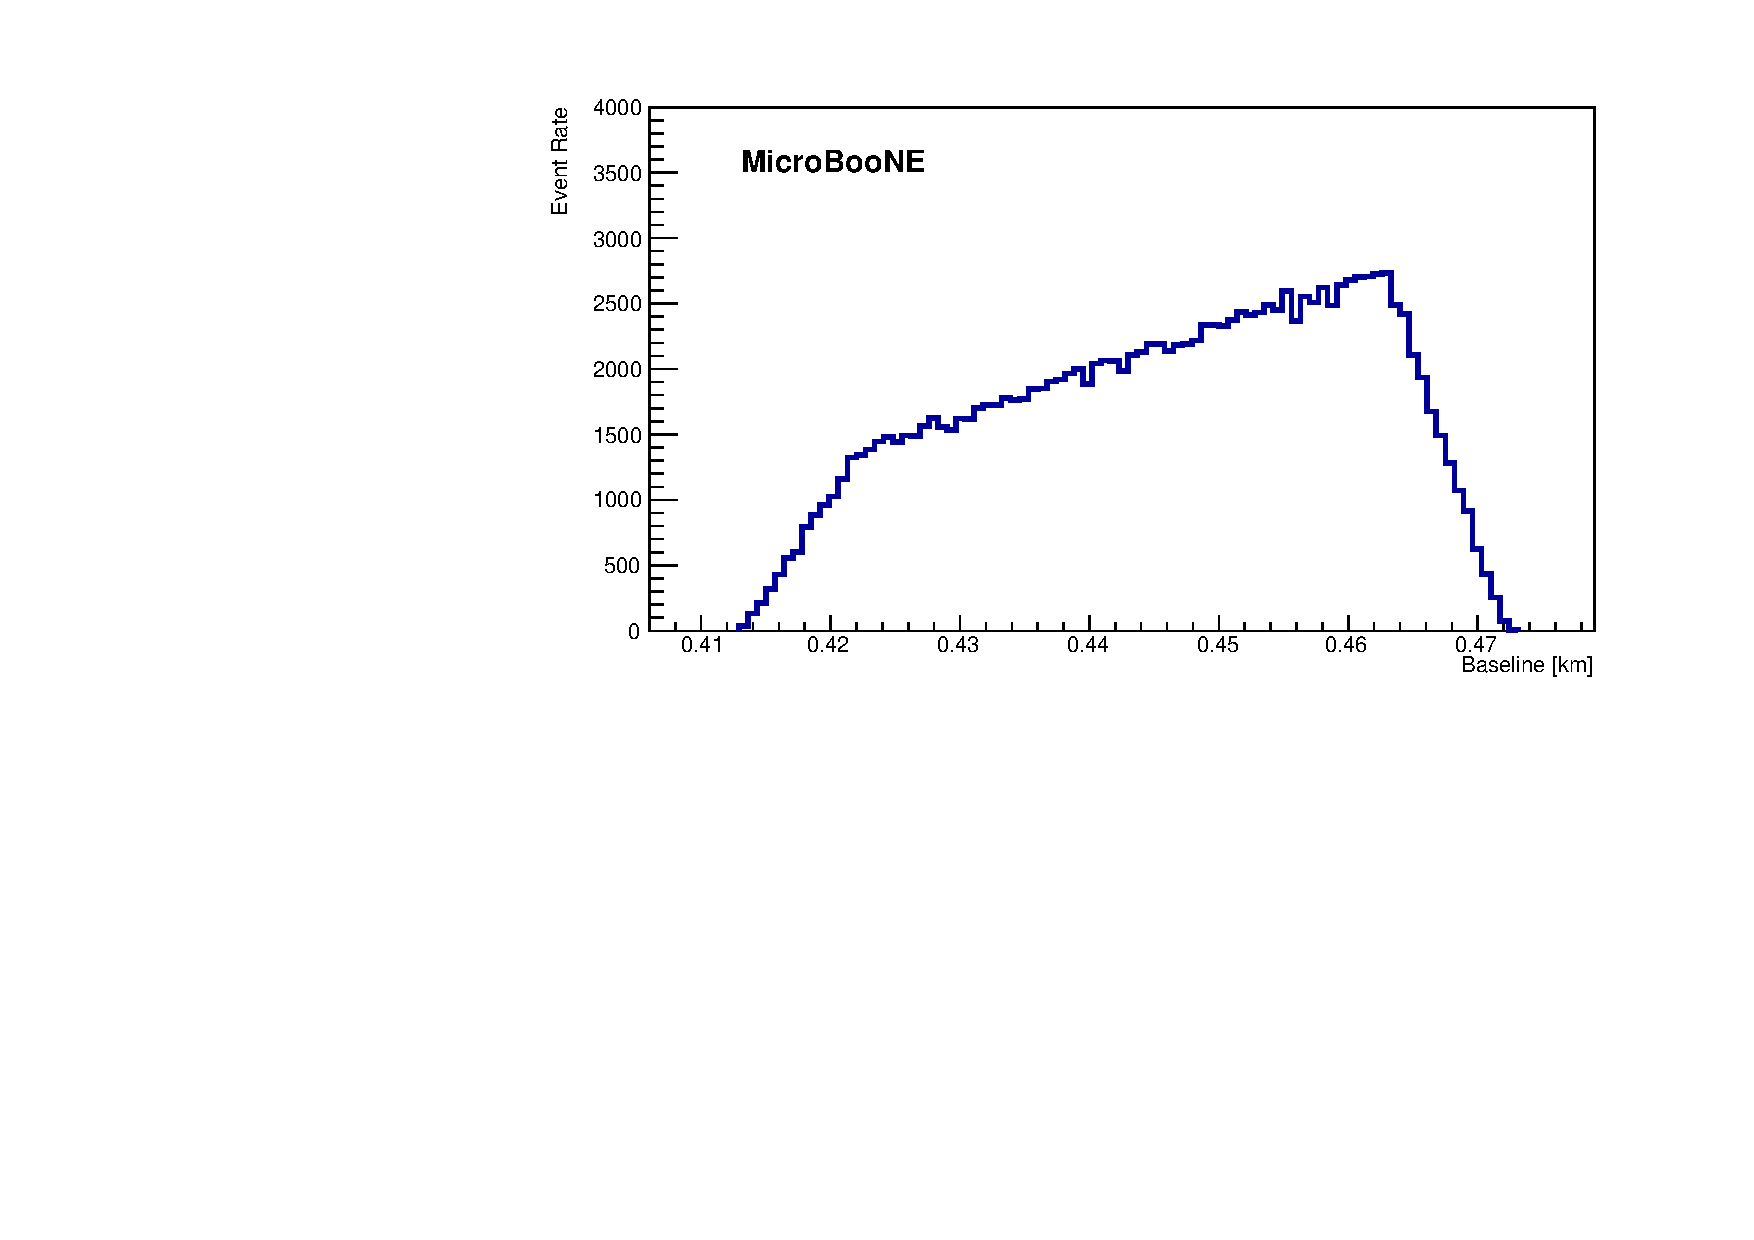
\includegraphics[width = 0.32\textwidth]{figures-chap5/MicroBooNE_numu.pdf}
    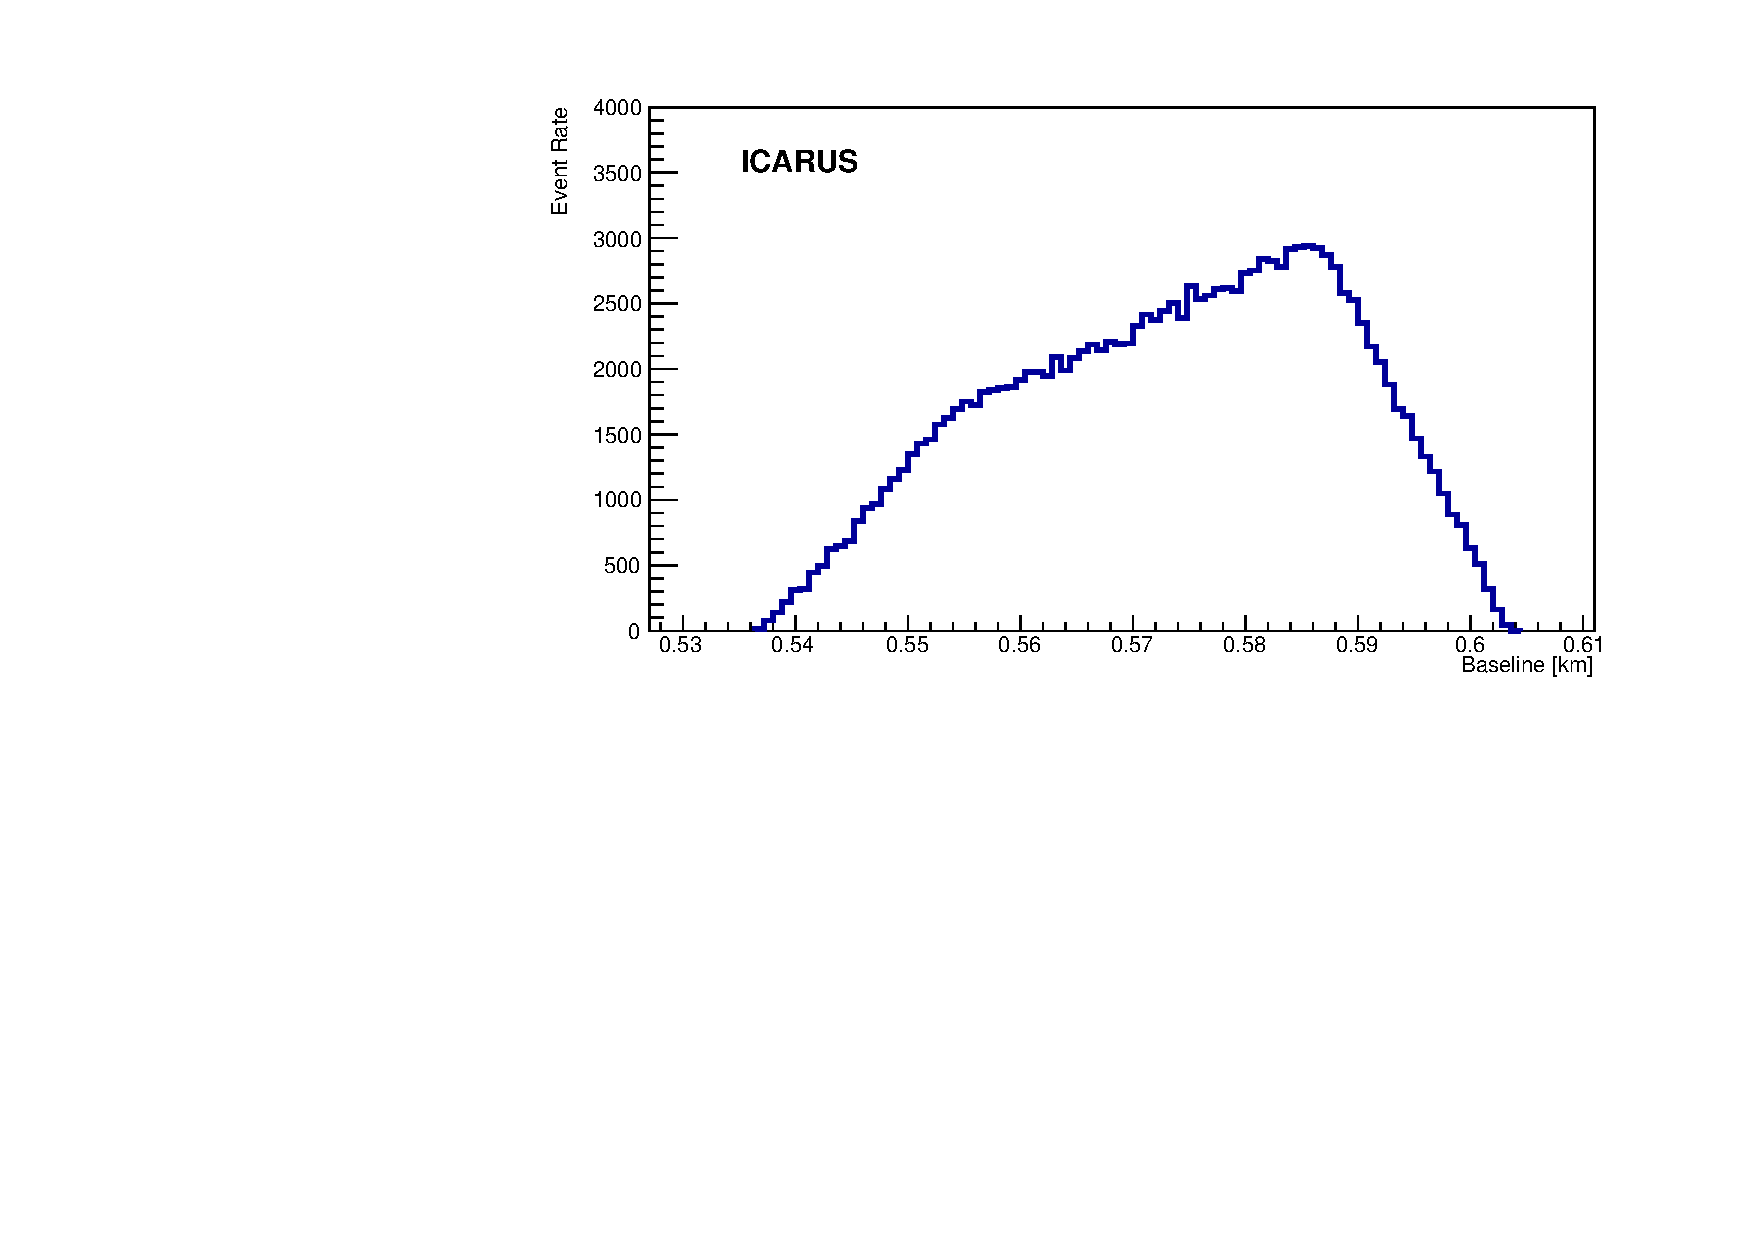
\includegraphics[width = 0.32\textwidth]{figures-chap5/ICARUS_numu.pdf}
    \caption{The baseline distribution of events in the \numu sample for each of the \gls{sbn} detectors.}
    \label{fig:numu_baseline}
\end{figure}

\begin{figure}[!h]
    \centering
    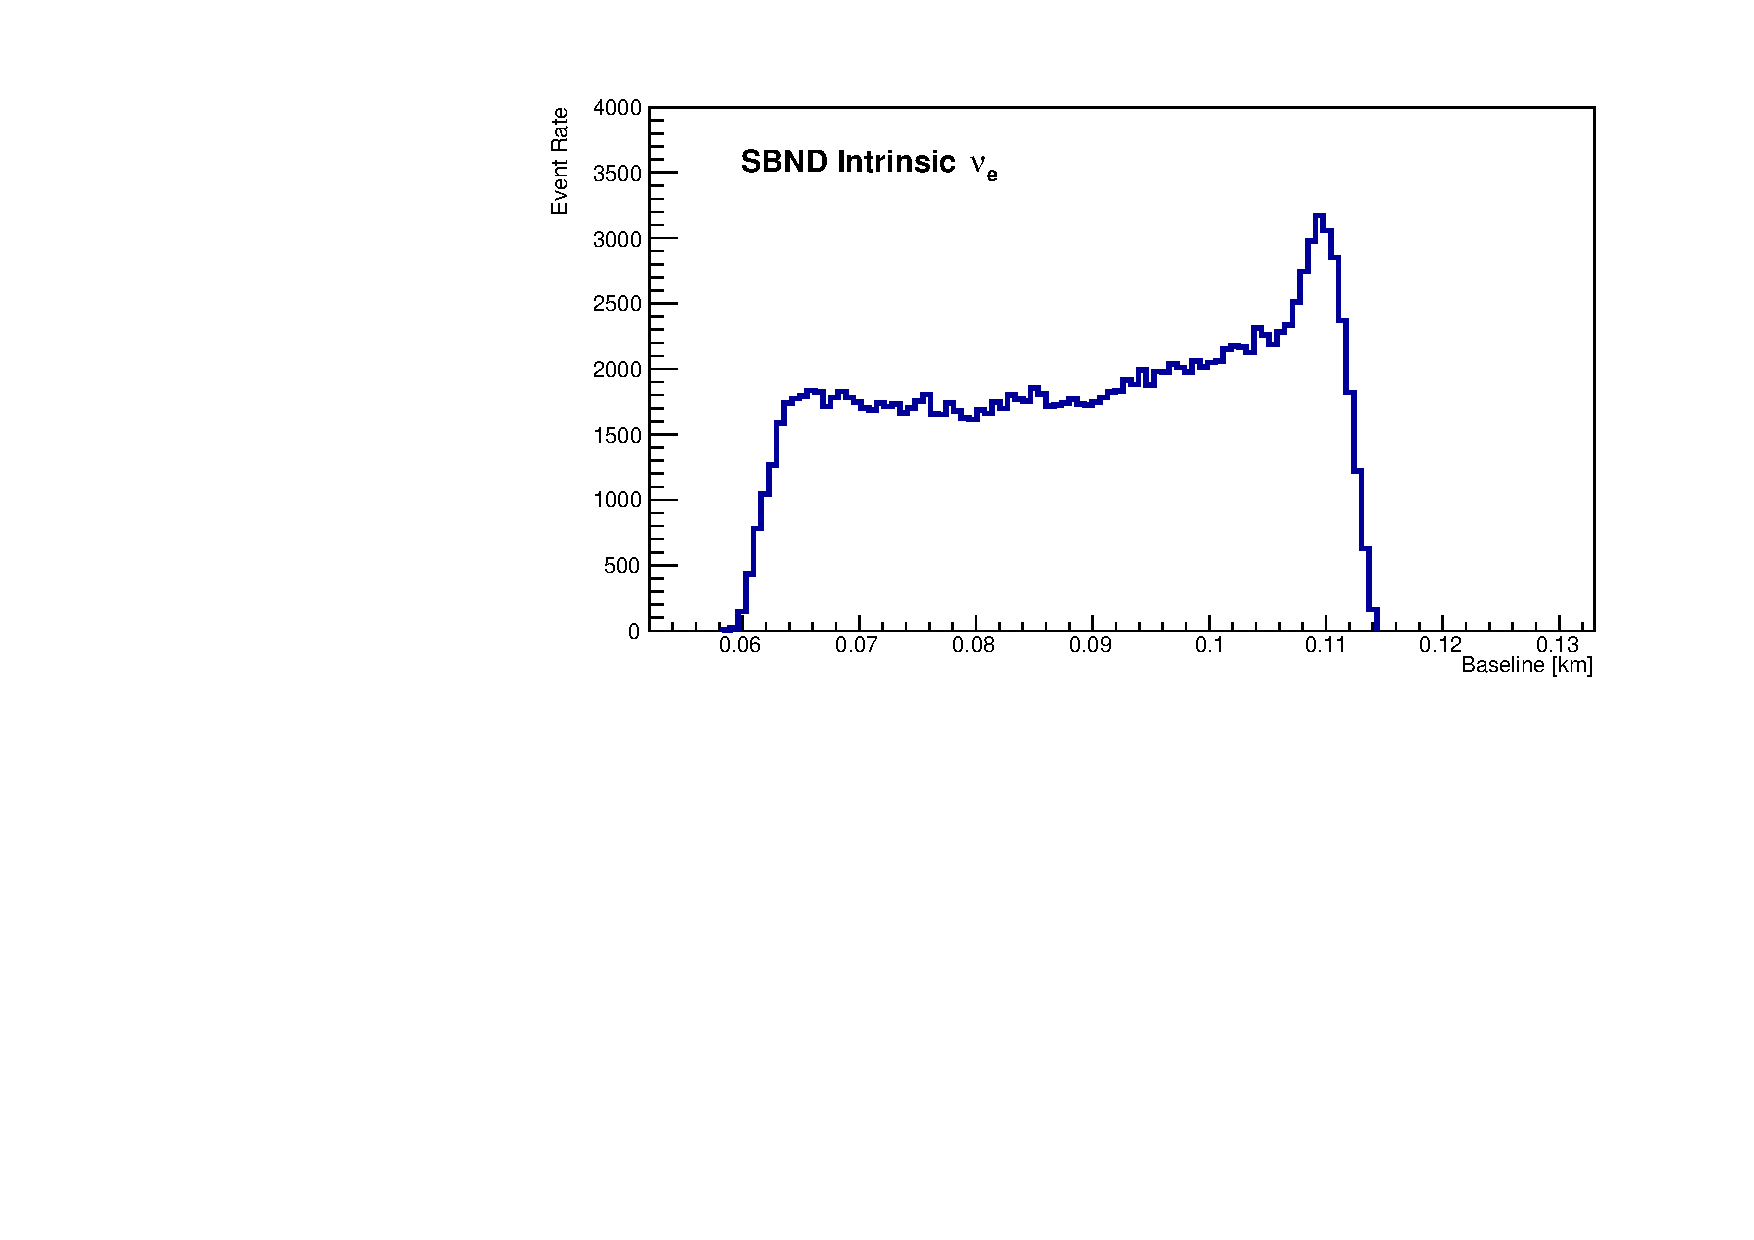
\includegraphics[width = 0.32\textwidth]{figures-chap5/SBND_intrinsic_nue.pdf}
    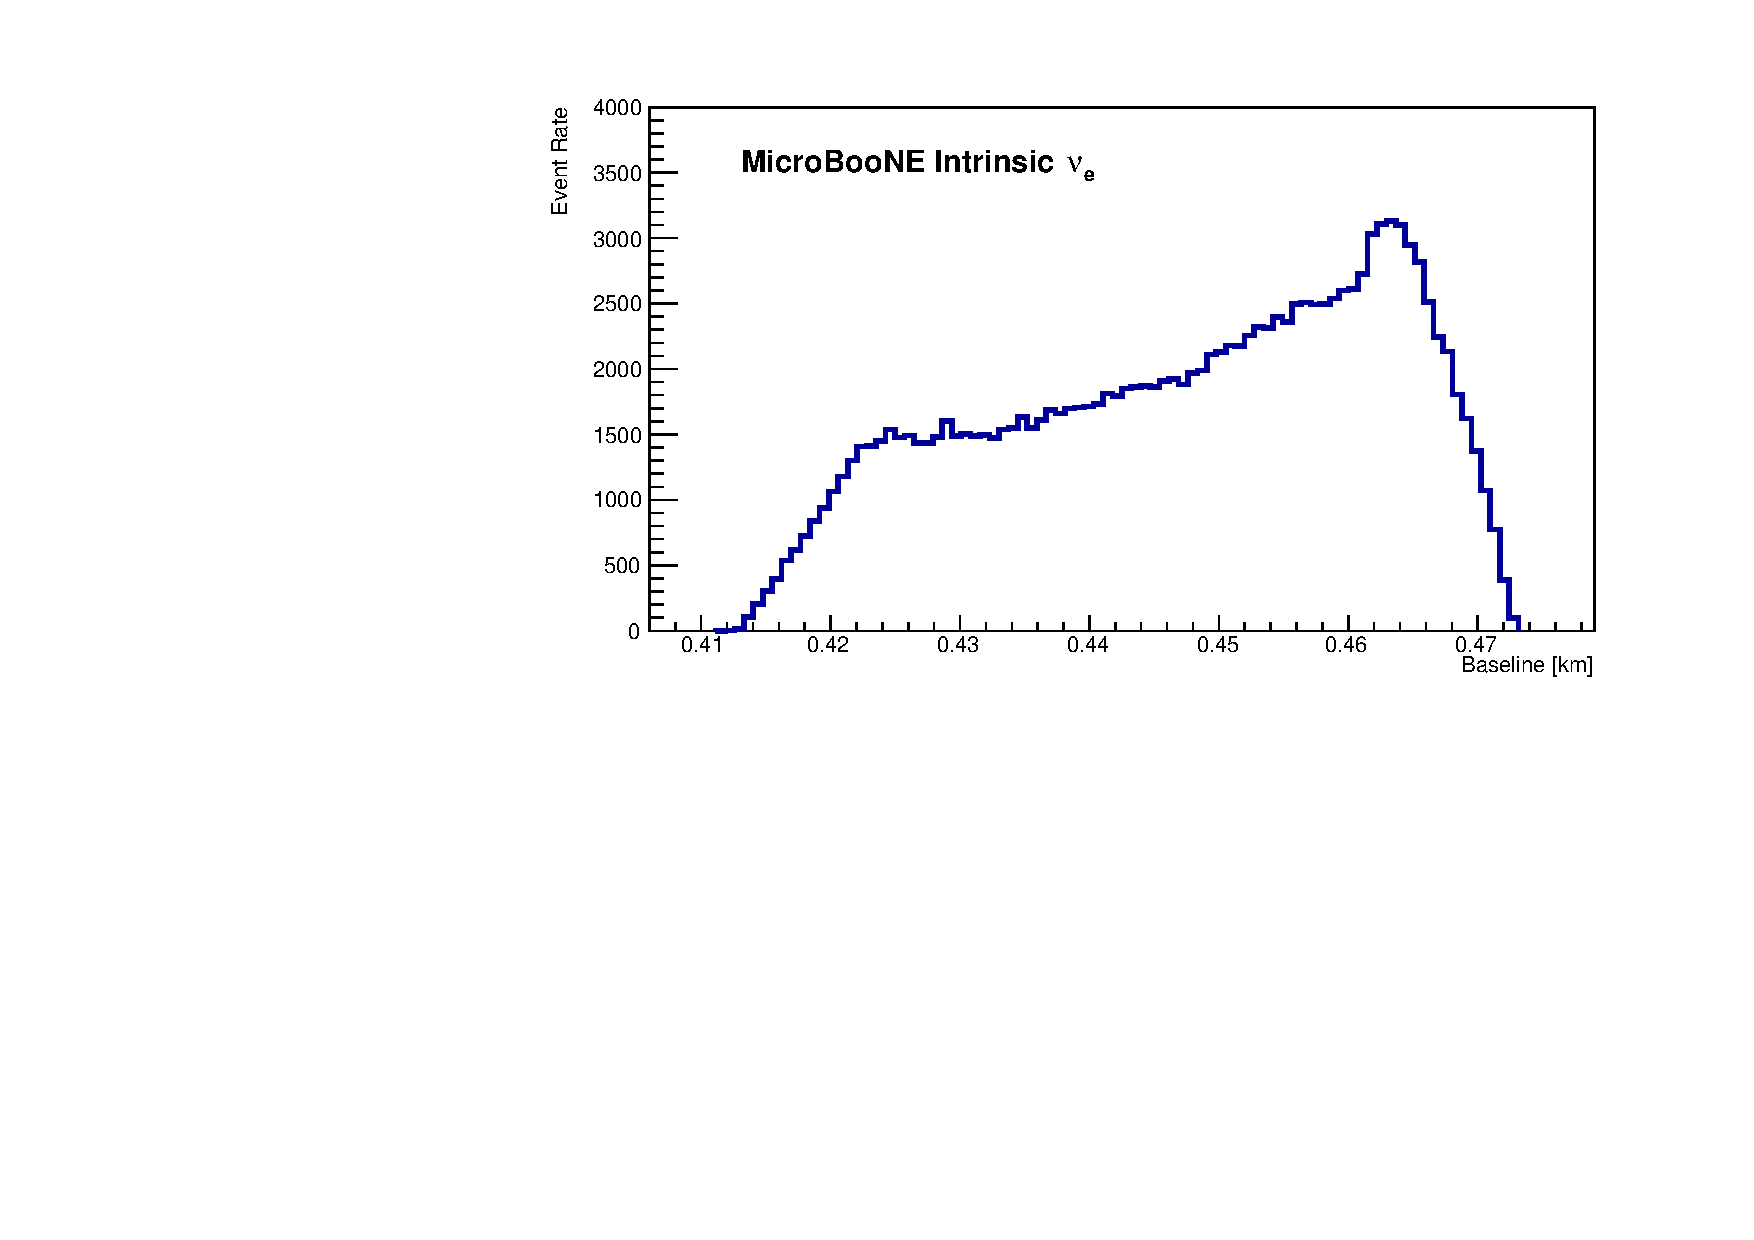
\includegraphics[width = 0.32\textwidth]{figures-chap5/MicroBooNE_intrinsic_nue.pdf}
    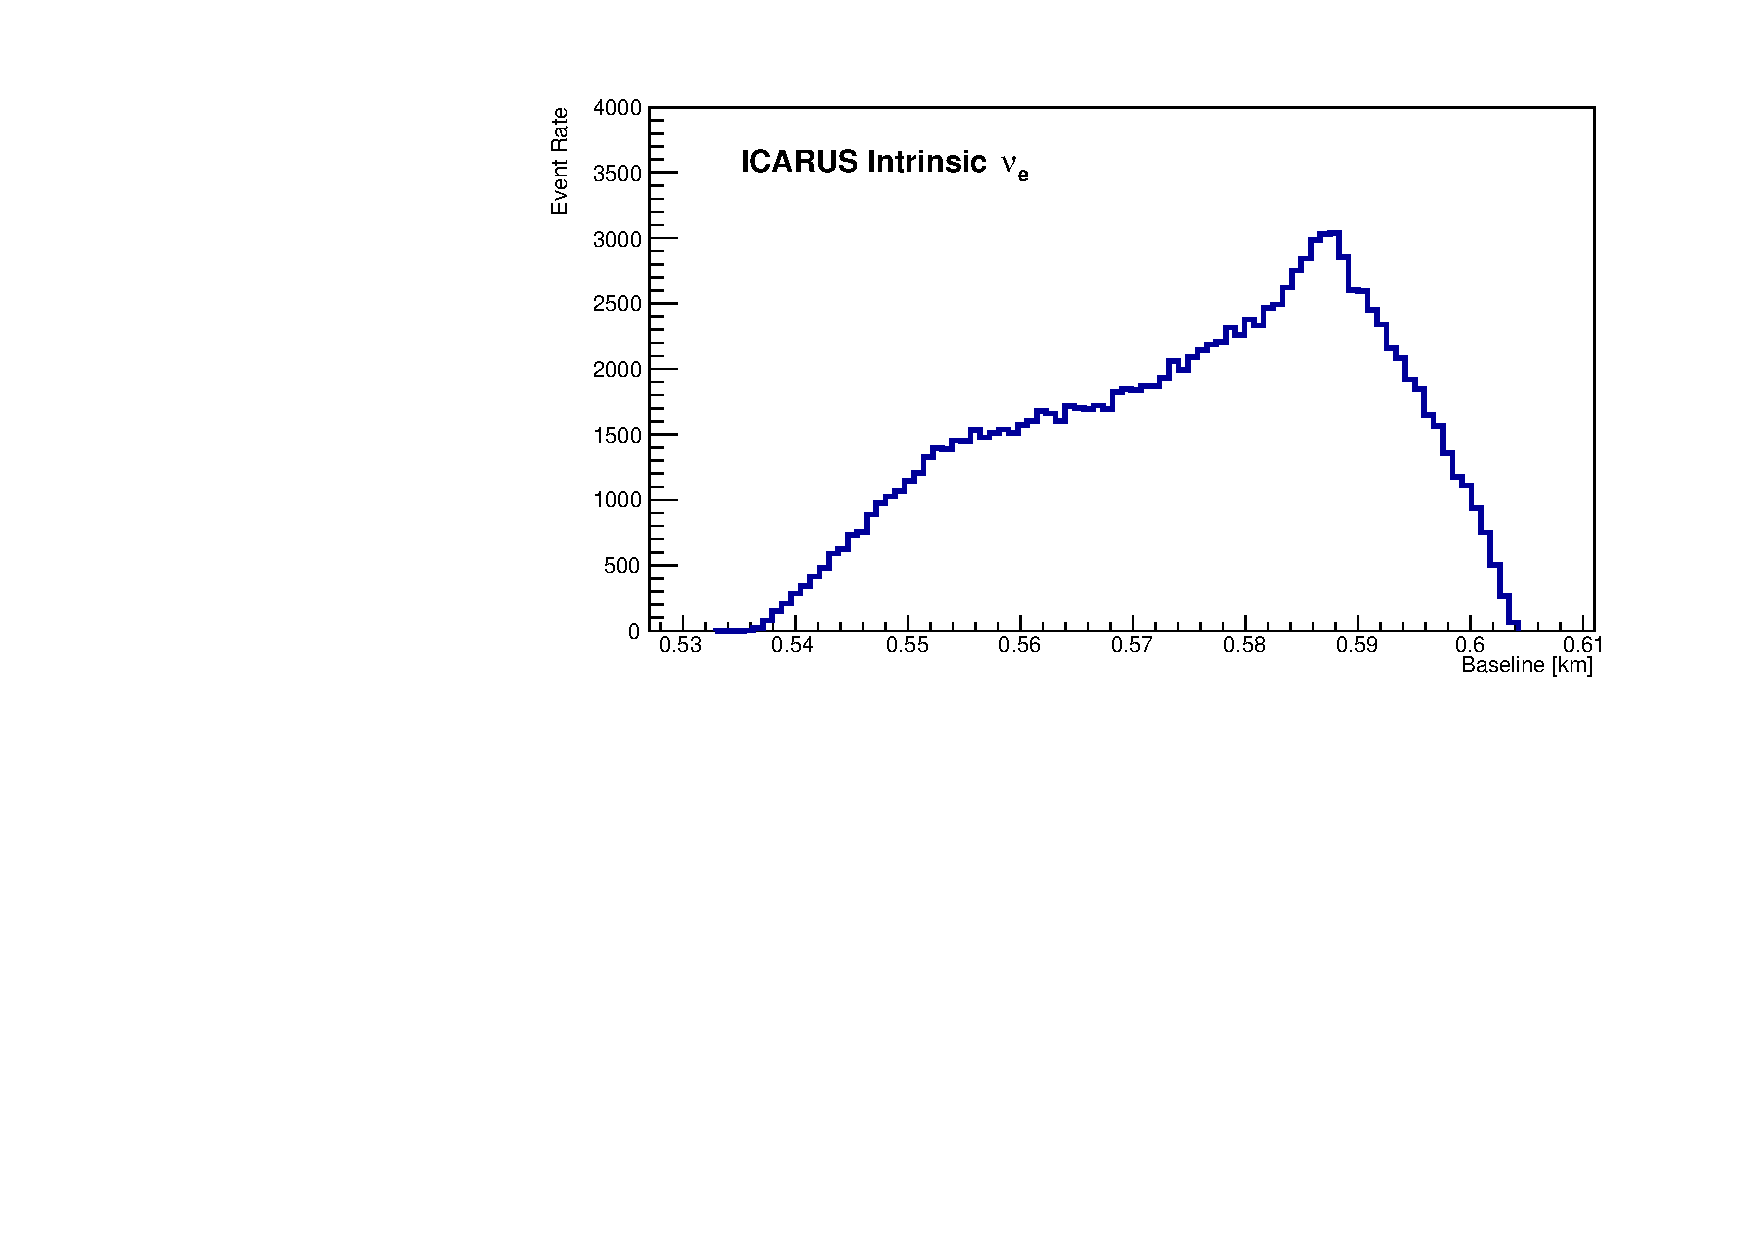
\includegraphics[width = 0.32\textwidth]{figures-chap5/ICARUS_intrinsic_nue.pdf} 
    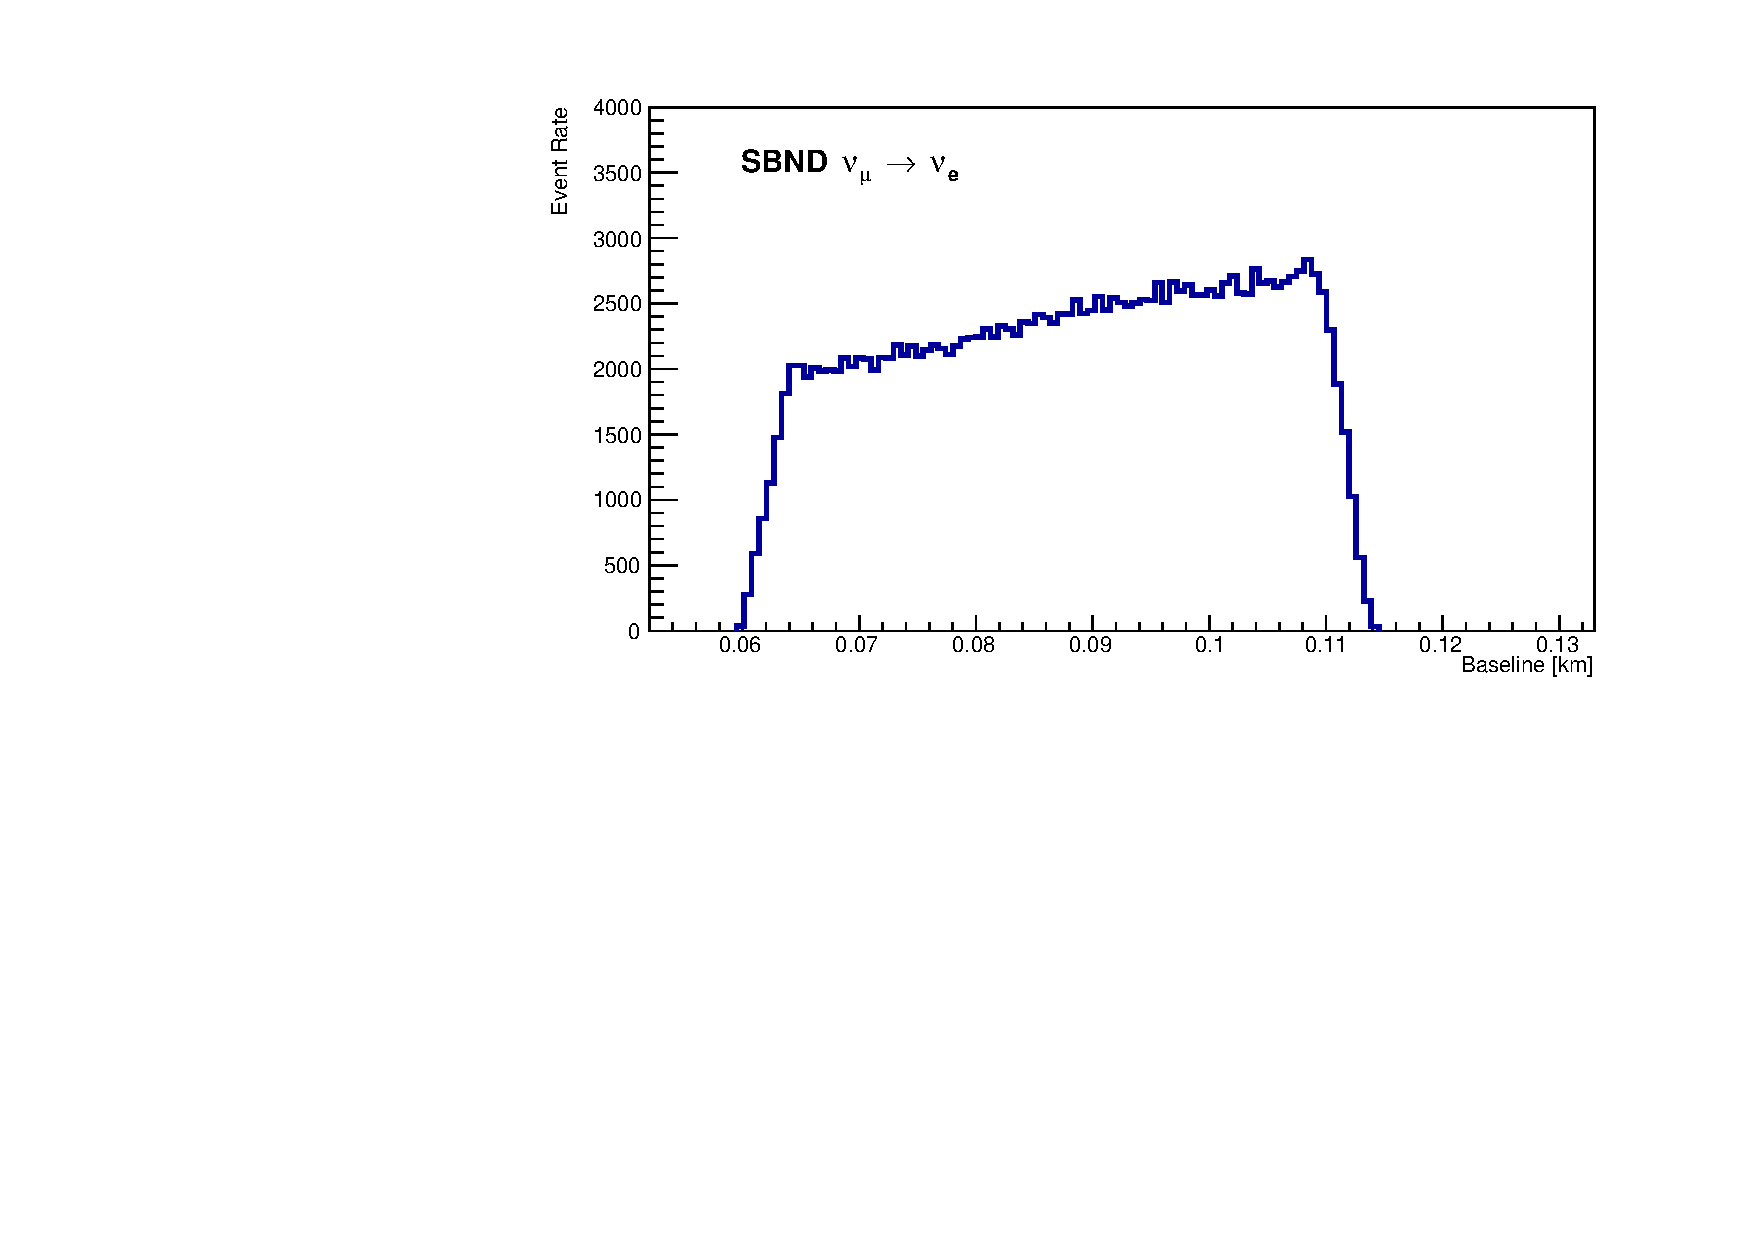
\includegraphics[width = 0.32\textwidth]{figures-chap5/SBND_osc.pdf}
    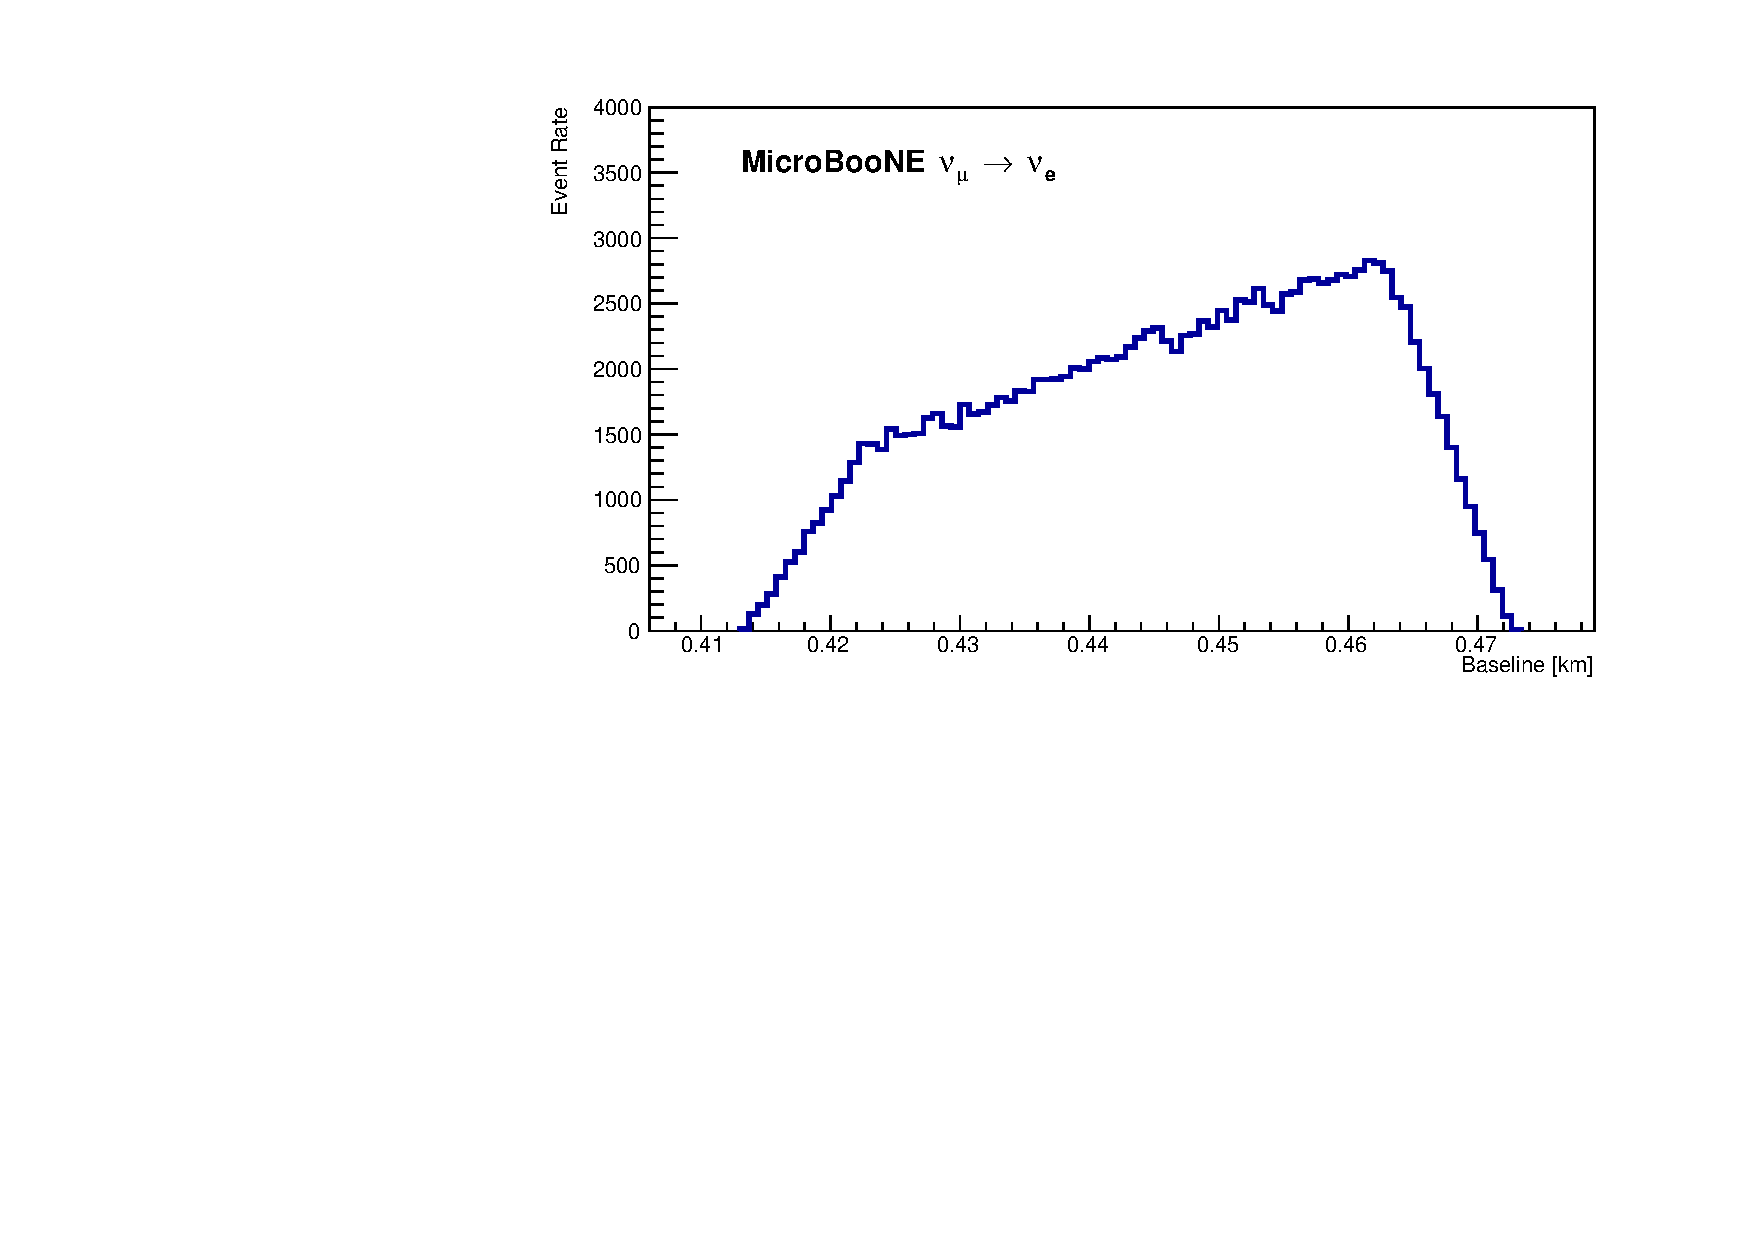
\includegraphics[width = 0.32\textwidth]{figures-chap5/MicroBooNE_osc.pdf}
    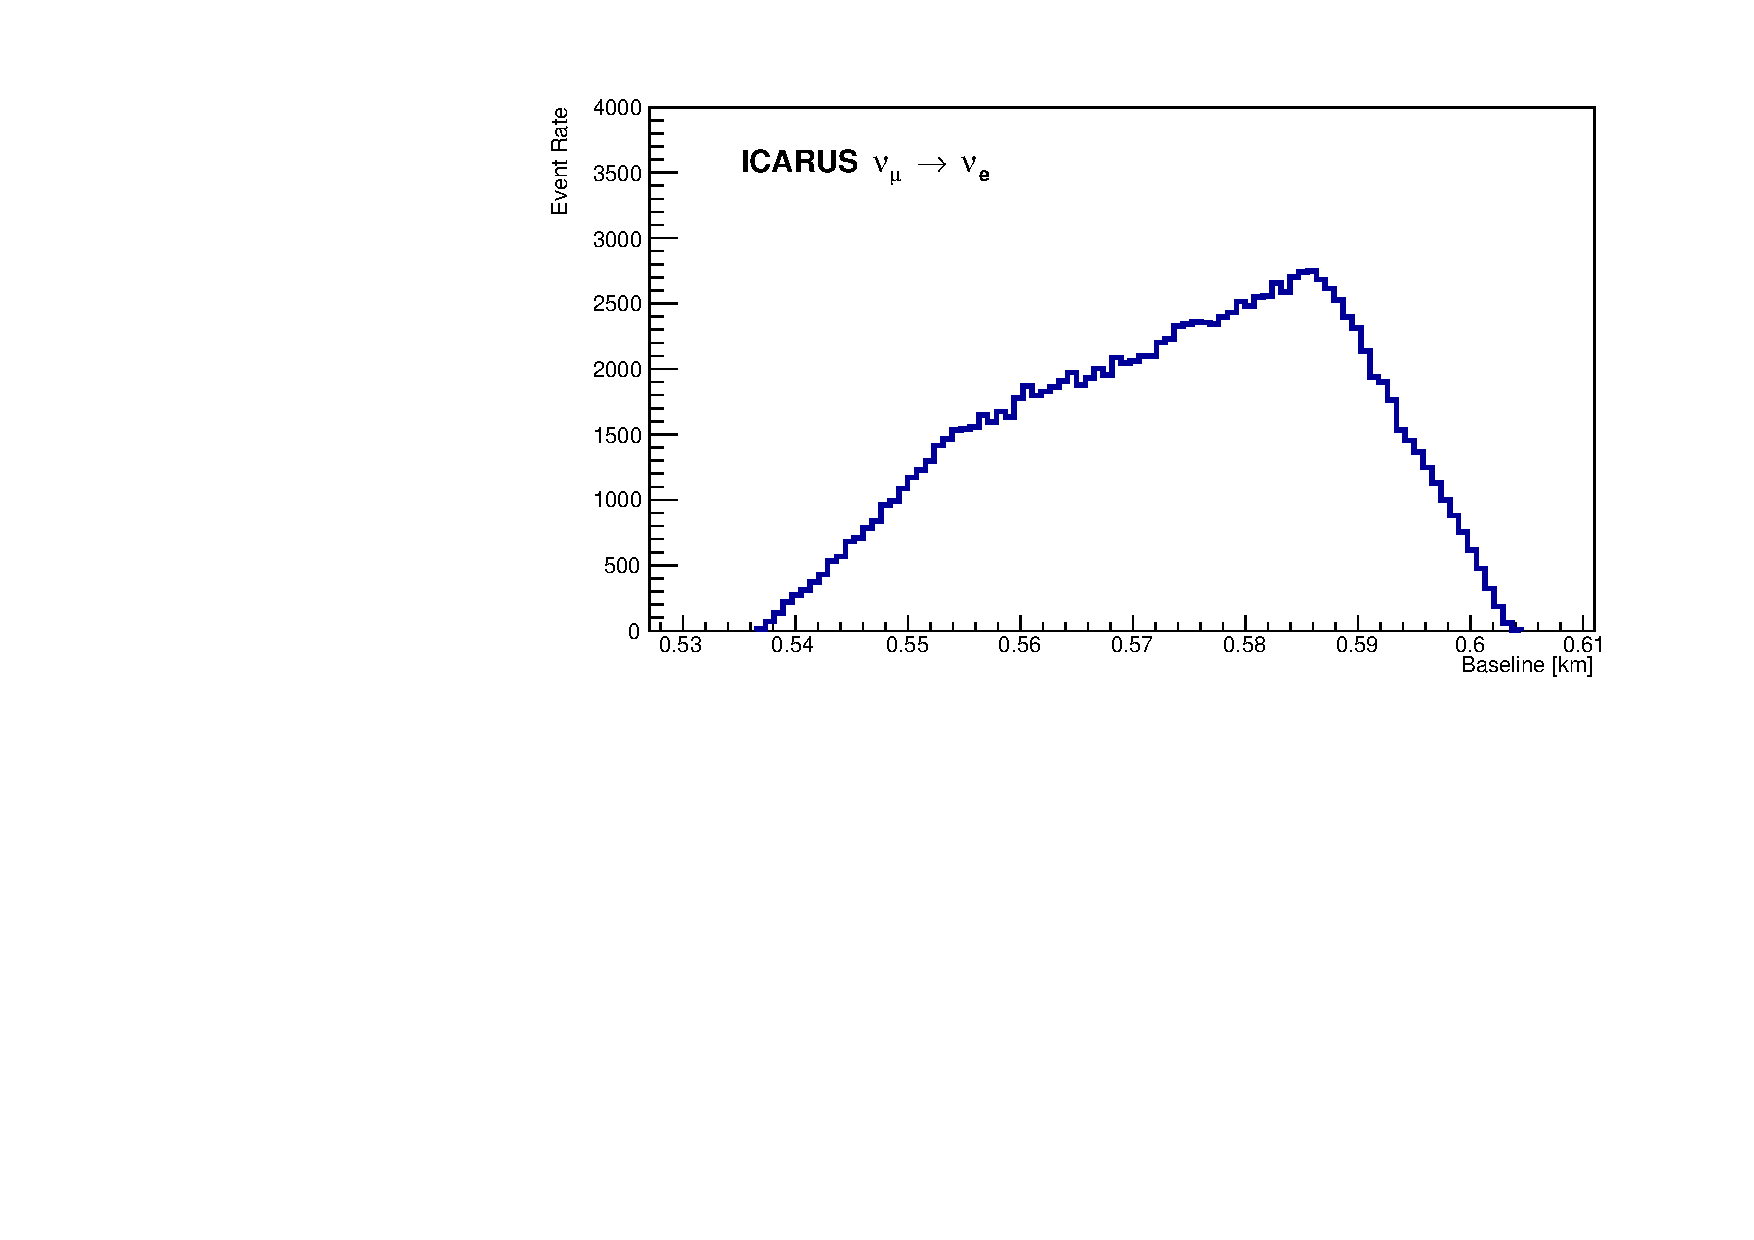
\includegraphics[width = 0.32\textwidth]{figures-chap5/ICARUS_osc.pdf}
    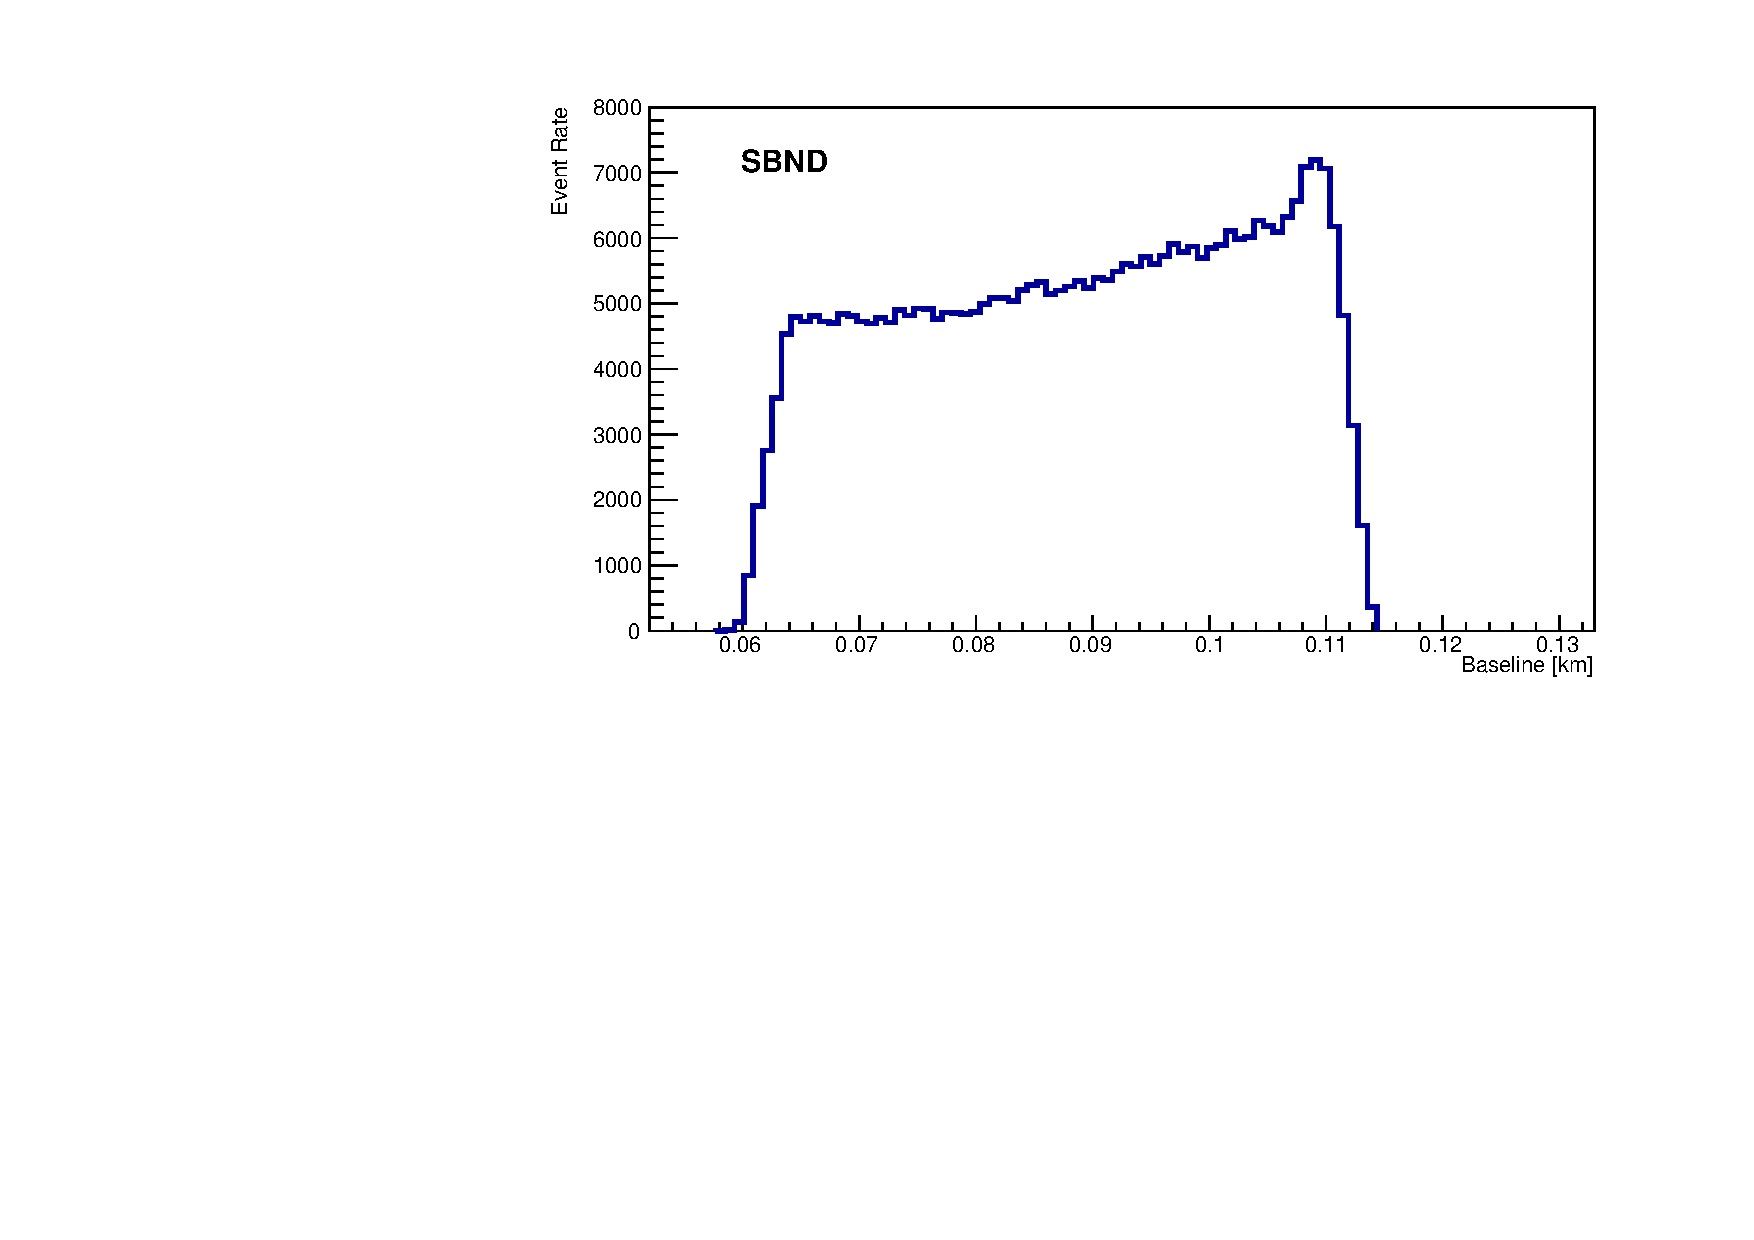
\includegraphics[width = 0.32\textwidth]{figures-chap5/SBND_nue.pdf}
    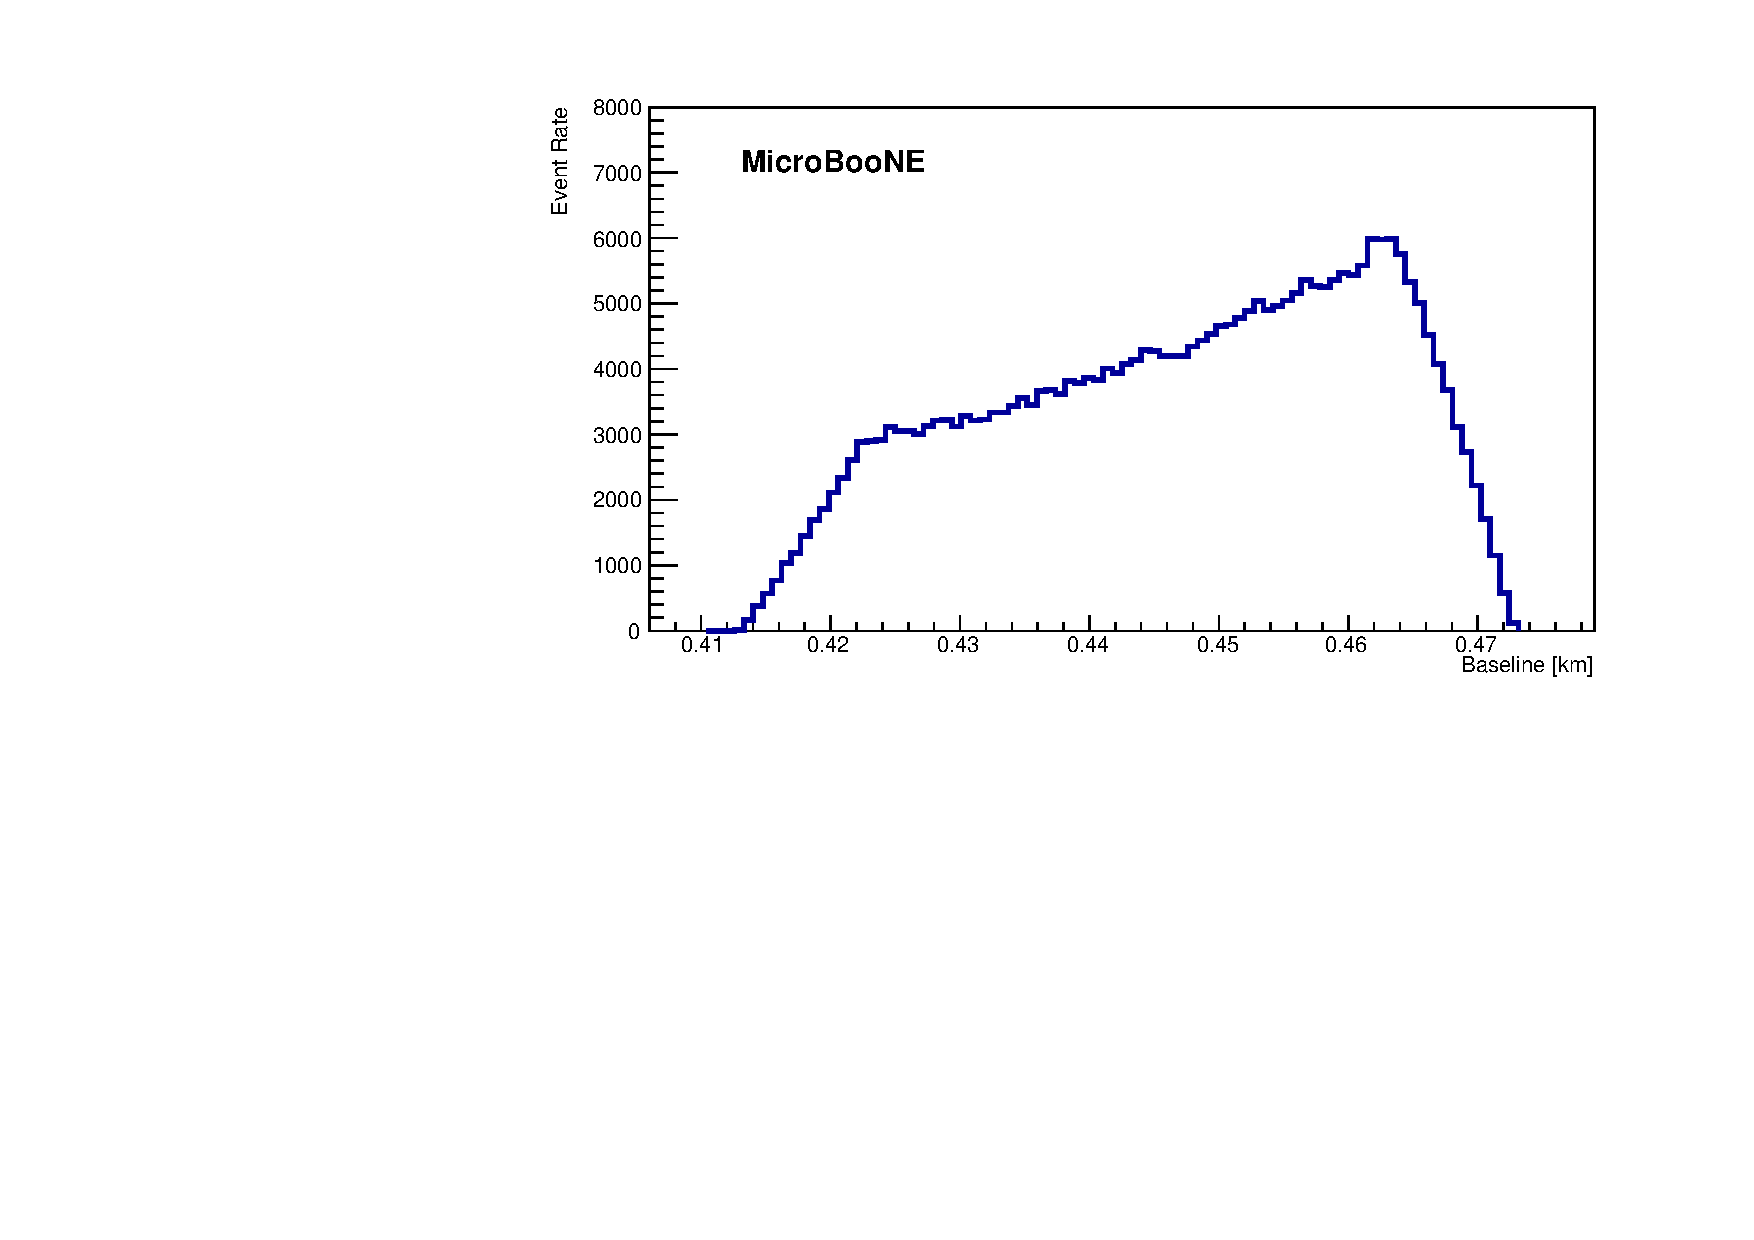
\includegraphics[width = 0.32\textwidth]{figures-chap5/MicroBooNE_nue.pdf}
    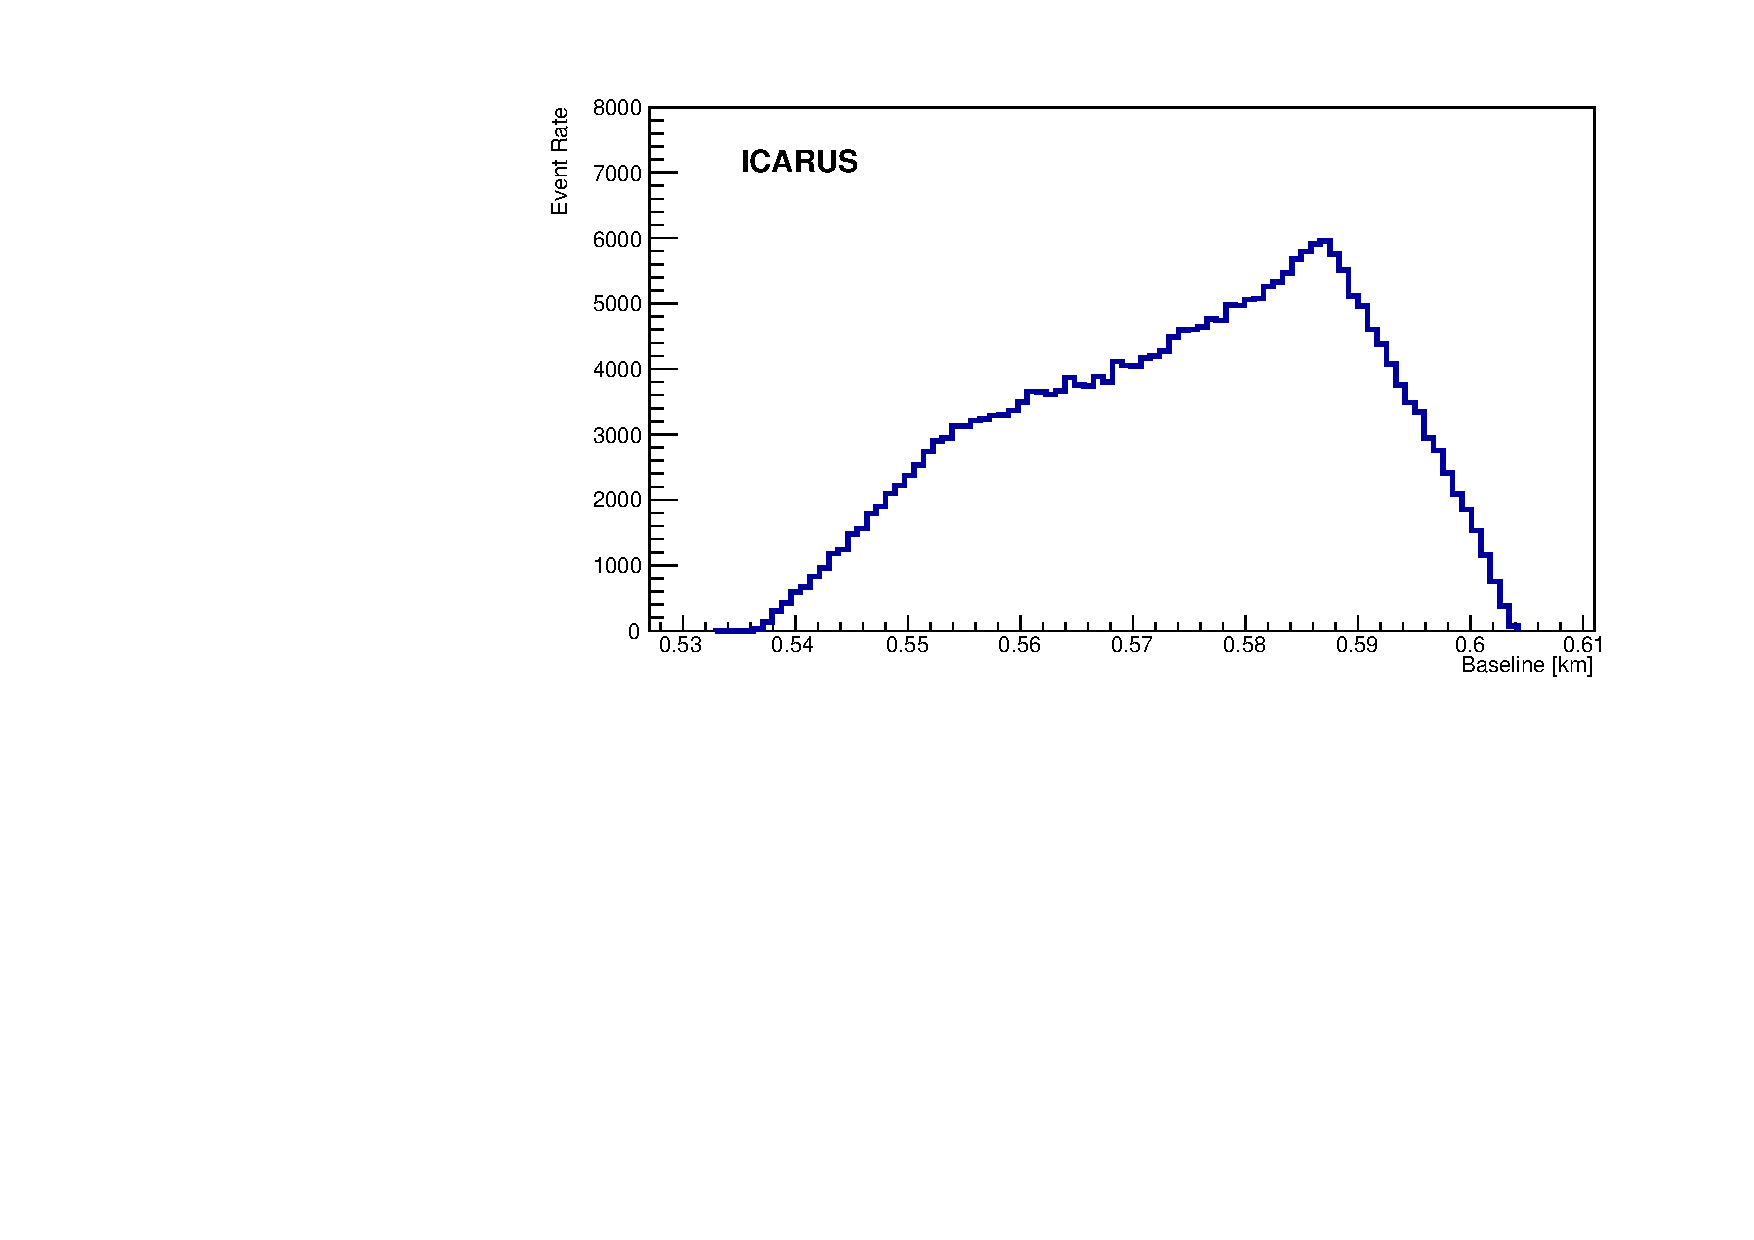
\includegraphics[width = 0.32\textwidth]{figures-chap5/ICARUS_nue.pdf}
    \caption{The baseline distribution of events in each of the \gls{sbn} detectors for the intrinsic \nue sample (Top), the oscillated \nue sample (Middle) and the overall \nue sample (Bottom). The overall sample is comprised of the events from the intrinsic \nue, oscillated \nue, the \numu events from \FigureRef{fig:numu_baseline} passing the \nue selection and the dirt and cosmic samples (which are not explicitly shown).
    The overall baseline distribution for events used in the \nue sample in each of the three \gls{sbn} detectors.}
    \label{fig:nue_baseline_dist}
\end{figure}

\begin{figure}[!h]
    \centering
    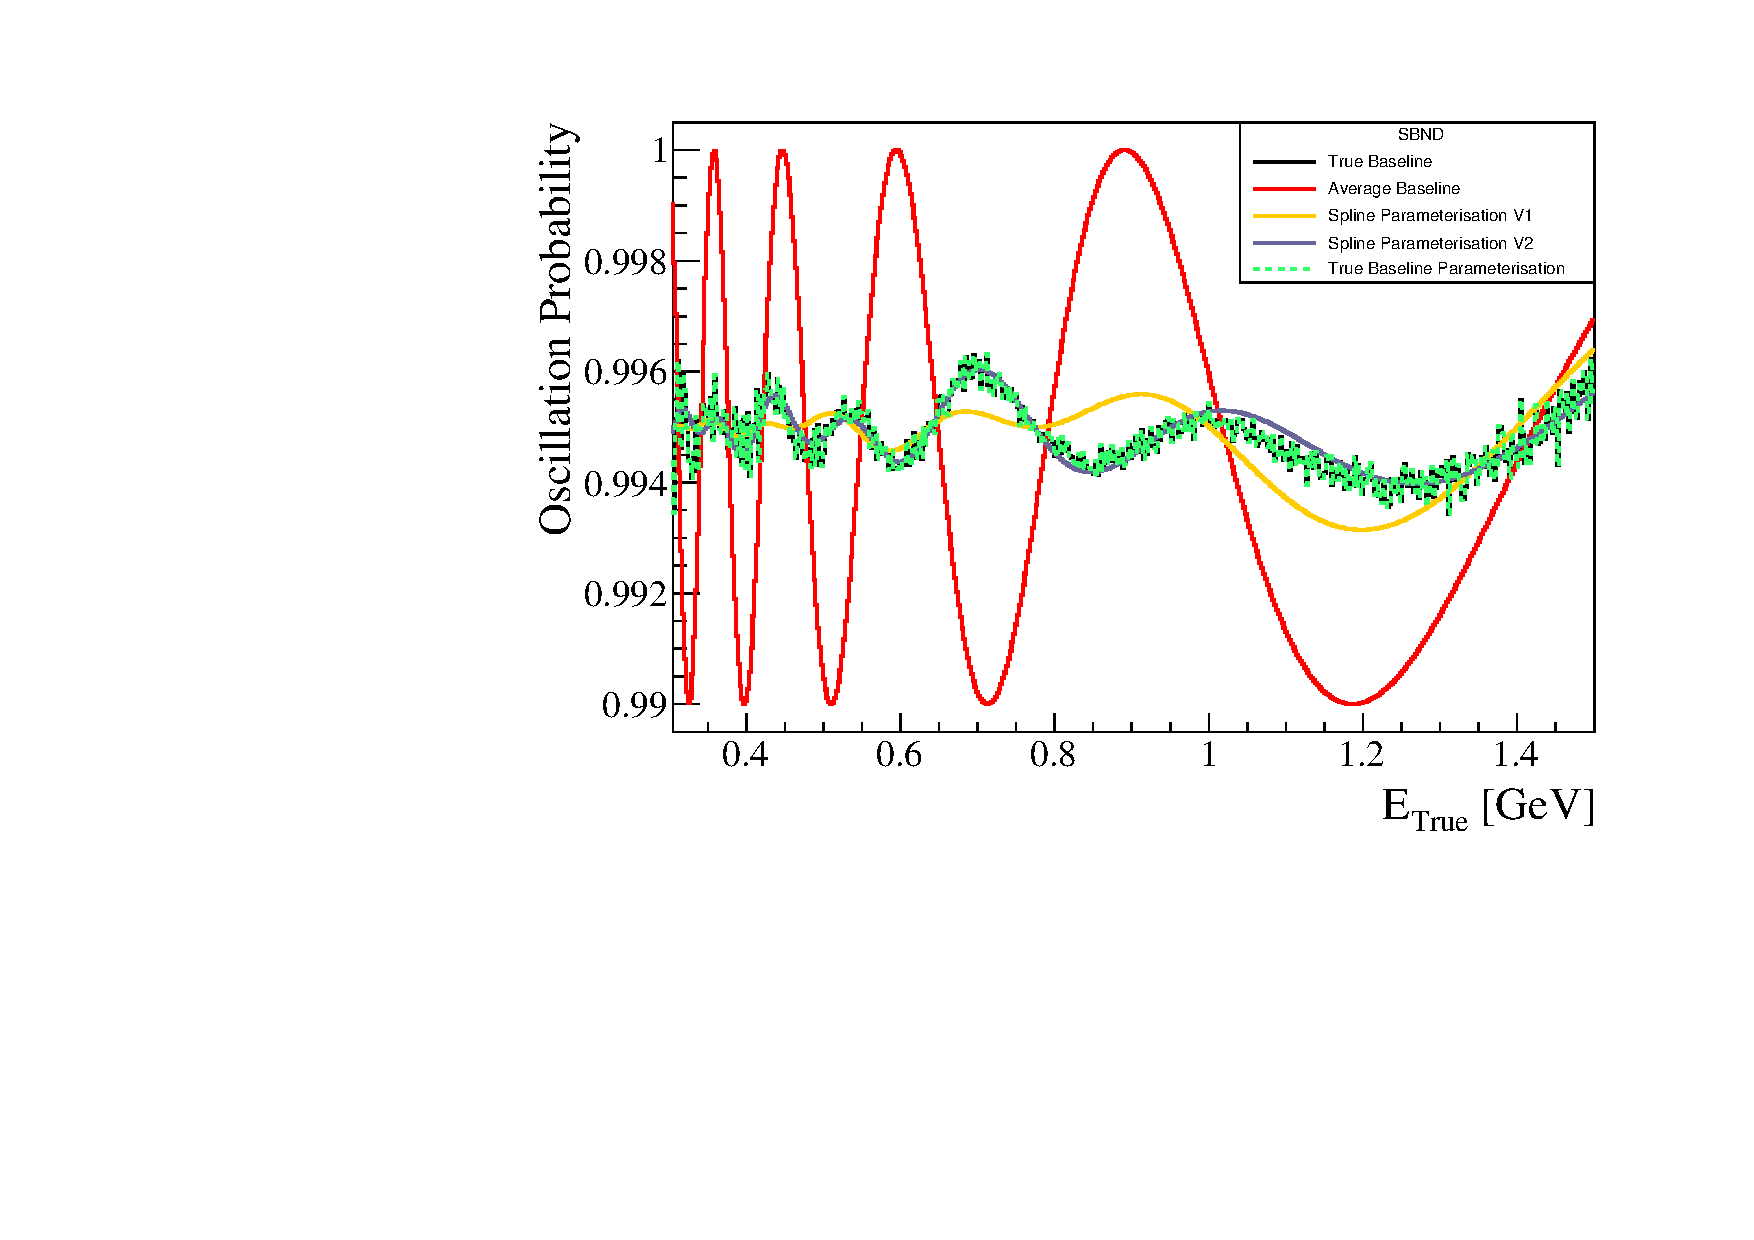
\includegraphics[width = 0.32\textwidth]{figures-chap5/osc_prob_sbnd.pdf}
    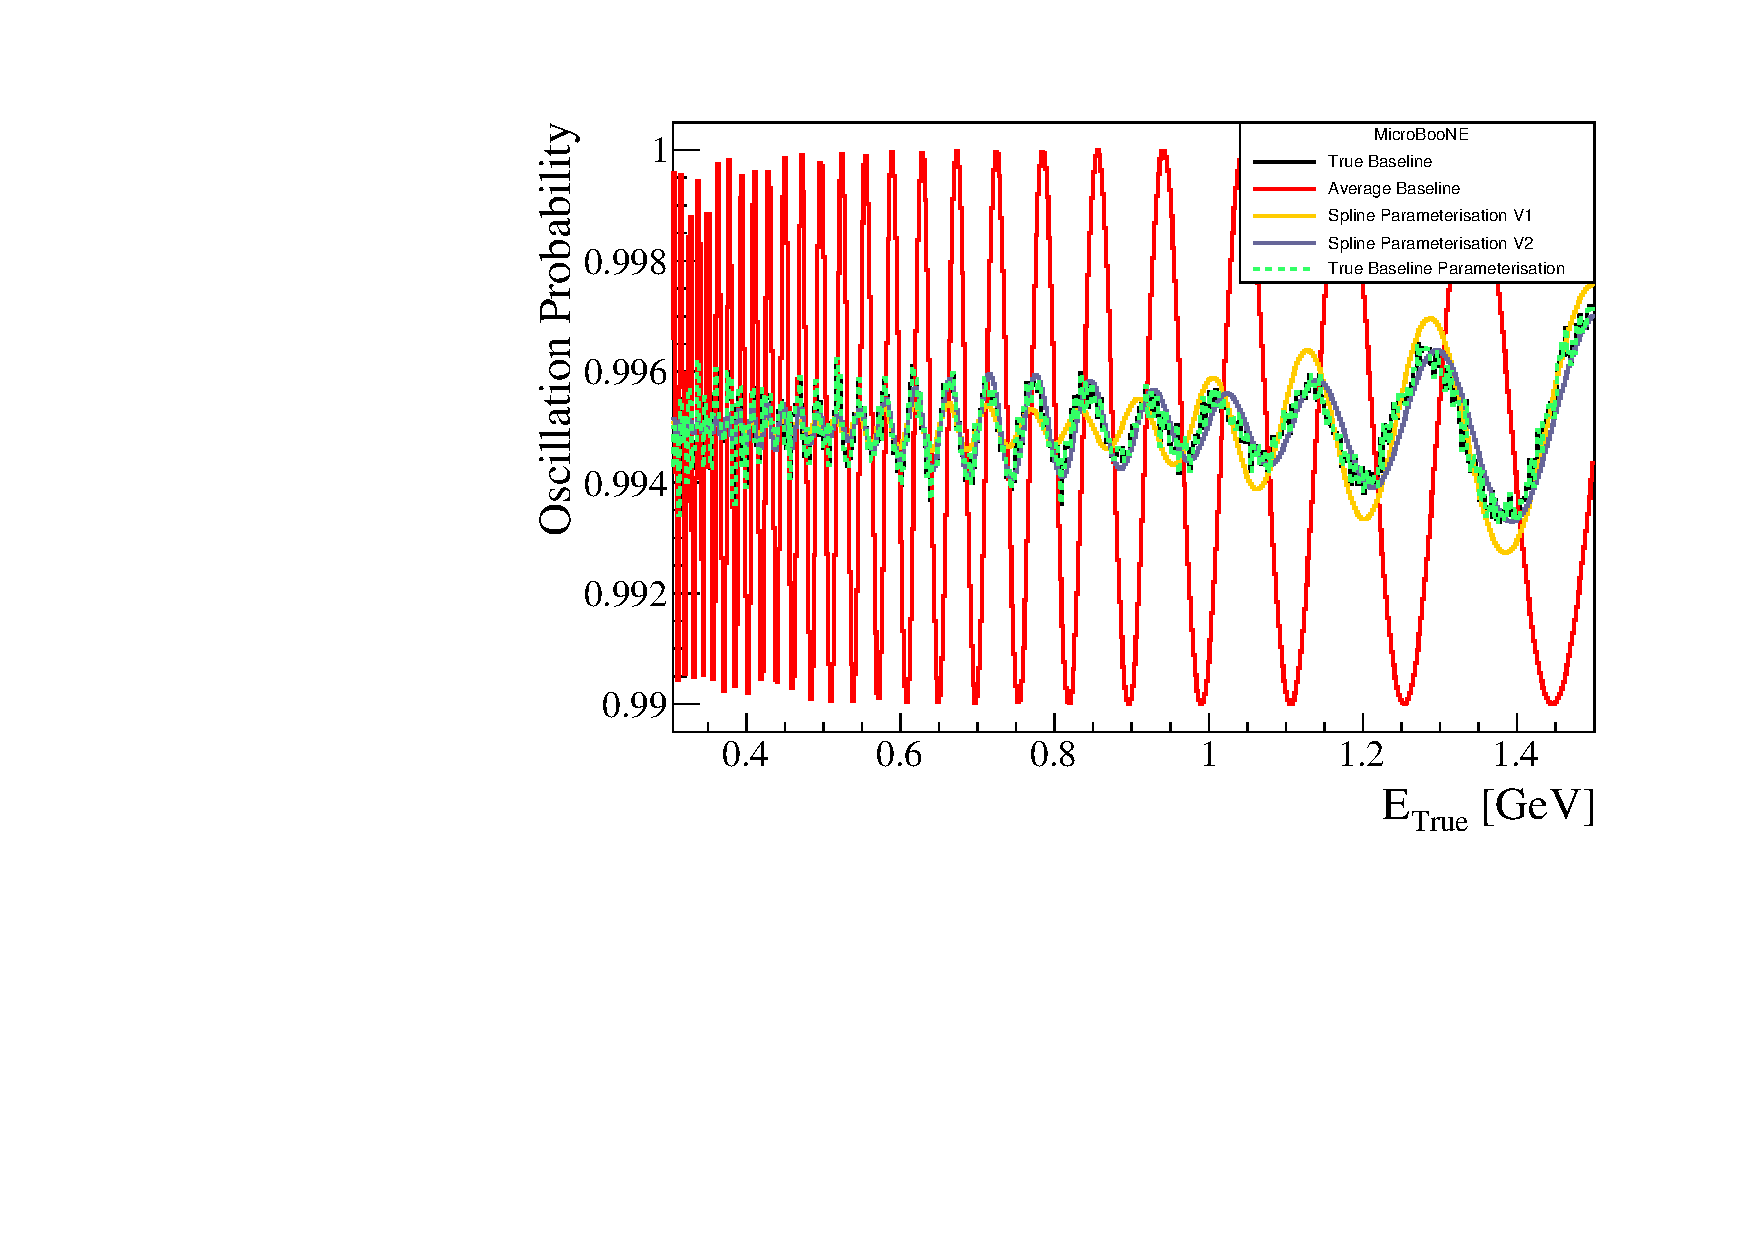
\includegraphics[width = 0.32\textwidth]{figures-chap5/osc_prob_uboone.pdf}
    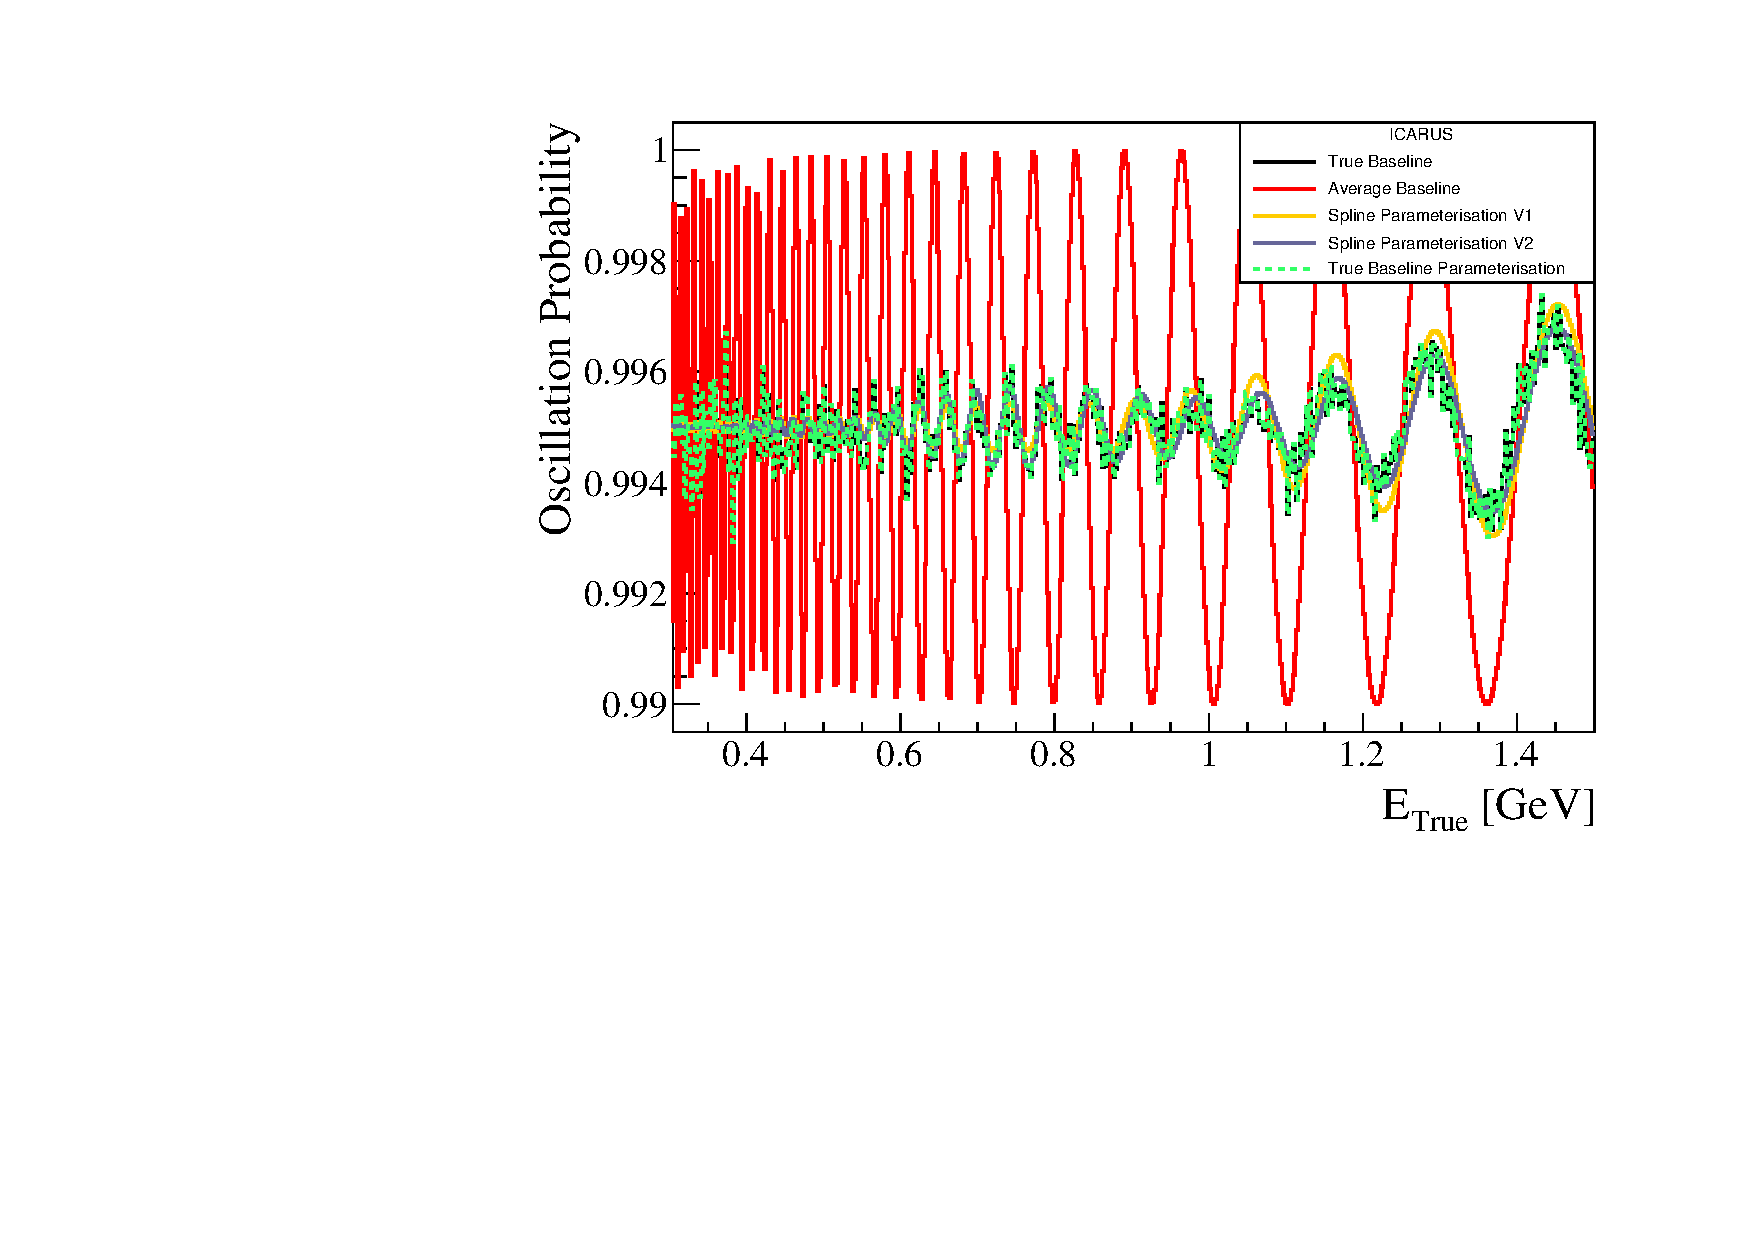
\includegraphics[width = 0.32\textwidth]{figures-chap5/osc_prob_icarus.pdf}
    \caption{The oscillation probability as a function of true neutrino energy for the \numu disappearance sample with oscillation parameters $sin^22\theta_{\mu\mu} = 0.01$ and $\Delta m^2_{41} = 50$ eV$^2$ in each \gls{sbn} detector. The results from using each baseline parametrisation are shown.}
    \label{fig:baseline_osc_probability}
\end{figure}

\subsection{Binning}\label{sec:binning}

The $\nu_\mu$ edge-to-edge binning has 21 bins in reconstructed neutrino energy which are bounded as follows:
\begin{itemize}
    \item 1 bin from 0.0-0.2 GeV,
    \item 2 0.1-GeV bins from 0.2-0.4 GeV,
    \item 12 0.05-GeV bins from 0.4-1.0 GeV,
    \item 2 0.25-GeV bins from 1.0-1.5 GeV,
    \item 3 0.5-GeV bins from 1.5-3.0 GeV and
    \item 1 bin from 3.0-10.0 GeV.
\end{itemize}

The $\nu_\mu$ edge-to-edge binning has 22 bins in true neutrino energy which are bounded as follows:
\begin{itemize}
    \item 1 bin from 0.00-0.30 GeV,
    \item 3 0.10-GeV bins from 0.30-0.60 GeV,
    \item 12 0.05-GeV bins from 0.60-1.20 GeV,
    \item 1 bin from 1.20-1.50 GeV,
    \item 3 0.50-GeV bins from 1.50-3.00 GeV,
    \item 1 bin from 3.00-5.00 GeV and
    \item 1 bin from 5.00-10.00 GeV.
\end{itemize}

The $\nu_e$ edge-to-edge binning has 12 bins in reconstructed neutrino energy which are bounded as follows:
\begin{itemize}
    \item 1 0.35-GeV bin from 0.00-0.35 GeV,
    \item 5 0.15-GeV bins from 0.35-1.10 GeV,
    \item 2 0.20-GeV bins from 1.10-1.50 GeV,
    \item 2 0.25-GeV bins from 1.50-2.00 GeV,
    \item 1 bin from 2.00-3.00 GeV and
    \item 1 bin from 3.00-10.00 GeV.
\end{itemize}

The $\nu_e$ edge-to-edge binning has 33 bins in true neutrino energy which are bounded as follows:
\begin{itemize}
    \item 2 0.25-GeV bin from 0.00-0.50 GeV,
    \item 15 0.05-GeV bins from 0.50-1.25 GeV,
    \item 15 0.25-GeV bins from 1.25-5.00 GeV and
    \item 1 bin from 5.00-10.00 GeV.
\end{itemize}



  \chapter{VALOR Oscillation Analysis Framework}
\label{chap:VALOR}

The VALOR framework is a neutrino fitting framework that was first developed for the \gls{t2k} experiment but has since been adapted to also cover, Hyper-Kamiokande, \gls{dune} and the \gls{sbn} program \cite{VALOR}.

Performing an analysis within VALOR involves a number of physics parameters that define a physics hypothesis (e.g. neutrino oscillations) and the relevant systematic uncertainties. Event rate predictions are constructed for the associated detector, beam and event sample. These predictions are constructed as a function of a kinematical variable for either a nominal scenario or with variations due to a physics hypothesis and/or systematic uncertainties. This approach allows for joint oscillation and systematic fits to be constructed from a binned likelihood fitting approach for a given event topology. Fits may be performed for individual detectors or for a combination of multiple detectors and may include any number of systematic uncertainties. 

\section{The VALOR Framework}\label{sec:VALOR_framework}

The data inputs used for an oscillation analysis are mainly provided in the form of \glspl{mct}, which provide a mapping between true and reconstructed variables. They are constructed following the full event processing chain which includes event simulation, reconstruction and selection. Since the \glspl{mct} include the effects from reconstruction and selection, it is not feasible to directly recreate them using only information on the flux, cross-section and efficiency. These \glspl{mct}, \textit{T}, encapsulate a number of quantities describing a given event and are listed below,

\begin{itemize}
    \item[b] -- Beam configuration e.g. neutrino or anti-neutrino mode,
    \item[d] -- Detector e.g. \gls{sbnd}, \gls{microboone} or \gls{icarus},
    \item[s] -- Topological event selection e.g. \nue CC-inclusive, \numu CC-inclusive,
    \item[m] -- True Reaction Mode e.g. \numu~CC QE, \nue~CC 1$\pi^{\pm}$,
    \item[r] -- A bin in multi-dimensional reconstructed kinematic space e.g. $E_{\nu, reco}$,
    \item[t] -- A bin in multi-dimensional true kinematic space e.g. $E_{\nu, true}$,
\end{itemize}

with $T = T_{d;b;s;m}(r, t)$. By combining \textit{T} with the necessary physics parameters, $\vec{\theta}$, and systematic parameters, $\vec{f}$, the predicted event rate, $n^{pred}_{d;b;s}$, may be expressed as
\begin{equation}
n_{d;b;s}^{pred}(r; \vec{\theta}; \vec{f}) =
   \sum_{m} \sum_{t}  P_{d;b;m}(t; \vec{\theta}) \cdot R_{d;b;s;m}(r,t; \vec{f}) \cdot T_{d;b;s;m}(r,t) \cdot N^{MC},
   \label{eq:valor_npred}
\end{equation}
where $P_{d;b;m}(t; \vec{\theta})$ represents the effect due to a physics hypothesis, $R_{d;b;s;m}(r,t; \vec{f})$ represents the response of a \gls{mct} bin to the systematic variations and $N^{MC} = \mbox{POT}_{b;d}^{data}/\mbox{POT}_{b;d}^{MC}$, which is the normalisation by which to scale the event rate to account for the POT which was used to construct the sample of neutrino events with respect to the nominal POT in the analysis. The variation due to systematic parameters is applied separately to each combination of beam, detector, topological selection and reaction mode in true-reconstructed space and is, therefore, dependant on, \textit{b, d, s} and \textit{m}. The dependence of $P_{d;b;m}(t; \vec{\theta})$ on \textit{d} and \textit{b} is due to \textit{d} and \textit{b} encapsulating the baseline information which is a component of the oscillation probability. The unoscillated \gls{cc} \glspl{mct} are weighted by the appropriate oscillation probability, $P_{\nu_{\alpha} \rightarrow \nu_{\beta}}$, to reflect the change in event rate due to neutrino oscillations. The \gls{nc} \glspl{mct} are left unweighted since they remain unchanged due to flavour oscillations. This distinction between \gls{cc} and \gls{nc} is encapsulated by \textit{m}, hence, $P_{d;b;m}(t; \vec{\theta})$ is required to also be dependent on \textit{m}. 

For $n_{d ; b ; s}^{obs}(r)$ observed events, the log likelihood, $\lnOf{\lambda_{d;b;s}(\vec \theta, \vec f)}$, is given by
\begin{equation}
    \lnOf{\lambda_{d;b;s}(\vec \theta, \vec f)} = - \mathlarger{\mathlarger{\sum_{b,d,s,r}}} \Bigg \{ \Big (n_{d;b;s}^{pred}(r,\vec{\theta},\vec{f})
    - n_{d ; b ; s}^{obs}(r) \Big) + n_{d ; b ; s}^{obs}(r) \cdot \lnOf{\frac{n_{d ; b ; s}^{obs}(r)}{n_{d ; b ; s}^{p r e d}(r , \vec{\theta} , \vec{f})}} \Bigg \}.
\end{equation}
An additional term is applied to penalise deviations from the nominal values of systematic parameters which is defined as,
\begin{equation}
    \lnOf{\lambda_{syst}(\vec{f})} = -\frac{1}{2} (\vec{f} - \vec{f}_0)^T \mathbf{V^{-1}} (\vec{f} - \vec{f}_0),
\end{equation}
where $\vec{f}_0$ is a vector containing the nominal value of all the systematic parameters and \textbf{V} is a covariance matrix containing the uncertainties of the systematic parameters \cite{VALOR_dune}. 

In the limit of large statistics, quantities of the form $-2\lnOf{\lambda}$ have a $\chi^2$ distribution, hence calculating the log-likelihood allows a goodness-of-fit test to be performed \cite{introduction_to_mathematical_statistics_book}. The total goodness-of-fit value is therefore given by,
\begin{equation}
    \chi^2_{tot} = -2(\lnOf{\lambda_{d;b;s}(\vec{\theta}, \vec{f})} + \lnOf{\lambda_{syst}(\vec{f})}).
\end{equation}

In order to create confidence regions, fits are performed between a certain \textit{Asimov} dataset and $n_{d;b;s}^{pred}$. The Asimov dataset is a dataset where all systematic parameters are set to their nominal values and serves as a proxy for data in cases where only simulations are considered. It has been shown that in the same limit as the $\chi^2$ approximation (in the limit of large statistics), the median of many toy \gls{mc} experiments is equivalent to the Asimov dataset. This allows the significance of a given hypothesis to be compared to the median one whilst only requiring one \textit{toy} experiment instead of needing to compute many toy \gls{mc} experiments \cite{Asimov_dataset}. Two types of confidence regions may be constructed; an \textit{exclusion} region and an \textit{allowed} region. Both regions show the area where the chosen model is either compatible or incompatible with the data. The difference is due to the input data which has either no oscillation signal (an exclusion region) or there is an injected signal (an allowed region). In the case of exclusion regions, the Asimov dataset corresponds to the case where no oscillations are observed which is the null-hypothesis and for allowed regions, the oscillation parameters are set to that of the injected signal. %For the \glspl{mct}, the oscillation parameters are set to a given value and the systematic parameters, if any, are allowed to float.

\section{Oscillation Channels Within SBN}

As was discussed in \SectionRef{sec:sbn_physics_capabilities}, the \gls{bnb} is \numu dominated with a small portion of \nue's present. In the presence of mixing with a light sterile neutrino 
this would result in the disappearance of some percentage of the \numu's due to oscillations. Additionally, \numu to \nue oscillations would result in the increase of the number of \nue's present. Finally, the number of intrinsic \nue's present in the \gls{bnb} coupled with the large event rate \gls{sbn} will detect means there are sufficient statistics to observe the disappearance of some \nue's due to oscillations. This results in three possible oscillation channels, \numu disappearance, \nue appearance and \nue disappearance. The mixing angles which determine their respective oscillation probabilities are shown in Equations (\ref{eqn:sinsq2thmumu} -- \ref{eqn:sinsq2thee}) which also imply that the oscillation channels are coupled (that is the presence of non-zero \nue appearance also requires non-zero \numu disappearance and \nue disappearance). Despite this, currently, the oscillation channels are treated completely independently. In principle oscillations involving \nutau are also possible, but due to the high energy threshold required these are usually not expected to be observed with any significant statistics. The energy range of the \gls{bnb} above the \nutau threshold is of the order 1\%, but since the statistics in \gls{sbnd} are large, this may be sufficient to observe \numu to \nutau appearance. Currently, this channel is not considered in the analysis but may be explored in future work \cite{tau_oscillations}.

The \numu disappearance as well as both the \nue channels have already been explored by a number of different experiments. This has led to tension due to the conflict between null-results from some experiments and the hints of possible mixing with light sterile neutrinos seen by others. 

The \numu disappearance channel has for example been investigated by \gls{minos}/\gls{minos}+, \gls{miniboone}/\gls{sciboone} and the IceCube experiment. The combined results from the \gls{miniboone} and \gls{sciboone} collaborations and a \gls{miniboone} only analysis (along with other experimental results) are shown on the left of \FigureRef{fig:miniboone_sciboone_minos}. The exclusion contours from \gls{minos} and \gls{minos}+ are shown on the right of \FigureRef{fig:miniboone_sciboone_minos}, with the black line representing the data and the dashed blue line being the expected sensitivity \cite{MiniBooNE/SciBooNE_numu_disapp_contour} \cite{MINOS_numu_disapp_contour}. It should be noted that the results from \gls{minos} are shown as a function of $\sin^2{\theta}$ instead of $\sin^2{2\theta}$ which is used for most other results. The results from 8 years of IceCube data are shown in \FigureRef{fig:icecube} along with other experimental results. The left plot is the 90\% C.L. allowed region, whereas the right plot is the 99\% C.L. exclusion contour. The star in each plot represents the best-fit point. The results depend on both $\theta_{24}$ and $\theta_{34}$, but the contours have been produced under the assumption that $\theta_{34} = 0$ \cite{IceCube_numu_disapp_contour}.

\begin{figure}[h!]
    \centering
    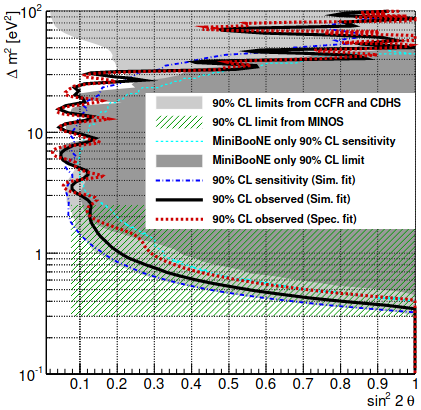
\includegraphics[width = 0.49\textwidth, height = 0.49\textwidth]{figures-chap6/external_limits/numu_disapp_MiniBooNE_SciBooNE.png}
    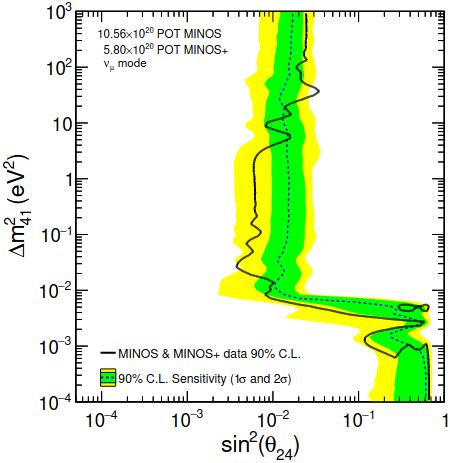
\includegraphics[width = 0.49\textwidth, height = 0.49\textwidth]{figures-chap6/external_limits/numu_disapp_Minos.png}
    \caption[\nue disappearance limits from the \gls{miniboone}/\gls{sciboone} and \gls{minos}/\gls{minos}+ experiments.]{Left: \numu disappearance exclusion contours obtained from the \gls{miniboone} and \gls{sciboone} experiments along with other experimental results \cite{MiniBooNE/SciBooNE_numu_disapp_contour}. Right: \numu disappearance exclusion contour from the \gls{minos}/\gls{minos}+ experiment \cite{MINOS_numu_disapp_contour}.}
    \label{fig:miniboone_sciboone_minos}
\end{figure}

\begin{figure}[h!]
    \centering
    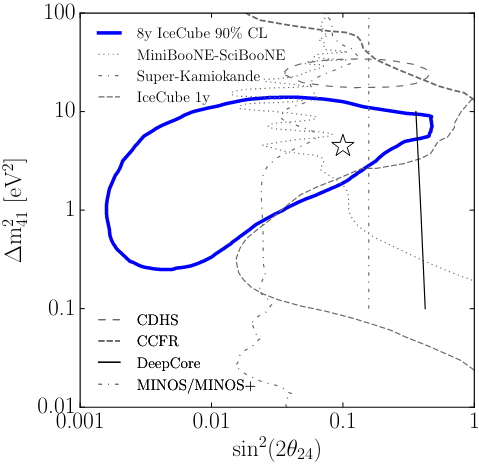
\includegraphics[width = 0.49\textwidth]{figures-chap6/external_limits/numu_disapp_icecube_90pct.png}
    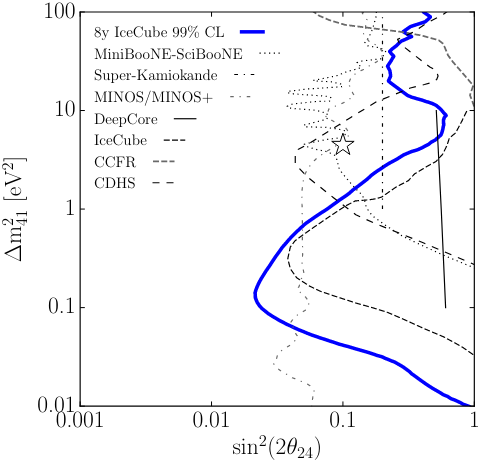
\includegraphics[width = 0.49\textwidth]{figures-chap6/external_limits/numu_disapp_icecube_99pct.png}
    \caption[\nue disappearance limits from the IceCube experiment.]{\numu disappearance results from the 8 years of IceCube data. The 90\% allowed region (Left) and the 99\% exclusion region are shown under the assumption that $\theta_{34} = 0$ \cite{IceCube_numu_disapp_contour}.}
    \label{fig:icecube}
\end{figure}

For the \nue appearance channel, the allowed regions from the \gls{lsnd} and \gls{miniboone} experiments are shown in \FigureRef{fig:nue_app_external}, along with exclusion contours from experiments including, \gls{icarus}, \gls{karmen}, NOMAD, OPERA and E776 (which is combined with solar neutrino data)\cite{LSND_excess}\cite{MiniBooNE_nue_app_contour}\cite{icarus_nue_app_contour}\cite{KARMEN_nue_app_contour}\cite{NOMAD}\cite{OPERA}\cite{E776}. The \gls{lsnd} result are produced from a combination of neutrinos from decay at rest (DaR) $\pi^+$ as well as decay in flight (DiF) pions meaning appearance of both \nue and \nuebar are considered. \gls{miniboone} also observed both neutrino and anti-neutrinos from the \gls{bnb}, whereas the \gls{karmen} experiment considered the oscillations of \numubar exclusively and the remaining experiments mentioned considered the oscillations of \numu exclusively \cite{LSND_KARMEN_nue_app_contour}.

\begin{figure}[!h]
    \centering
    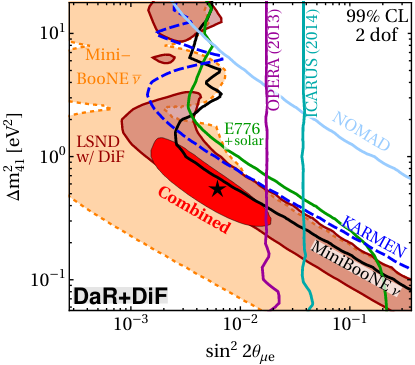
\includegraphics[width = \largefigwidth]{figures-chap6/external_limits/nue_app_combo.png}
    \caption[\nue appearance limits from the \gls{lsnd}, \gls{miniboone}, \gls{icarus}, \gls{karmen}, NOMAD, OPERA and E776 experiments.]{\nue appearance allowed regions from the \gls{lsnd} and \gls{miniboone} experiments and exclusion contours from the \gls{icarus}, \gls{karmen}, NOMAD, OPERA and E776 experiments \cite{LSND_KARMEN_nue_app_contour}.}
    \label{fig:nue_app_external}
\end{figure}

Finally, the \nue disappearance channel has been investigated with allowed regions being obtained from gallium and reactor experiments and exclusion regions being obtained from \nue-carbon interaction data and solar neutrino data. Additionally, the near detector of the \gls{t2k} experiment has provided both allowed and excluded regions which are shown in the left plot of \FigureRef{fig:nue_disapp_external}. An overlay of the \gls{t2k} exclusion region along with the other experimental results are shown in the right plot of \FigureRef{fig:nue_disapp_external}, all of which are shown at the 95\% CL. In both cases, the coloured star and circles correspond to the best-fit point of a given result \cite{T2K_nue_disapp_contour}. 

\begin{figure}[!h]
    \centering
    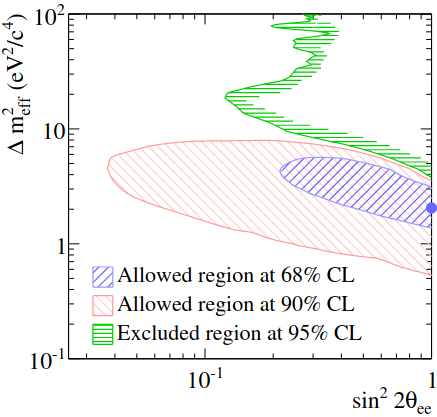
\includegraphics[width = 0.49\textwidth, height = 0.35\textwidth]{figures-chap6/external_limits/nue_disapp_external_T2K.png}
    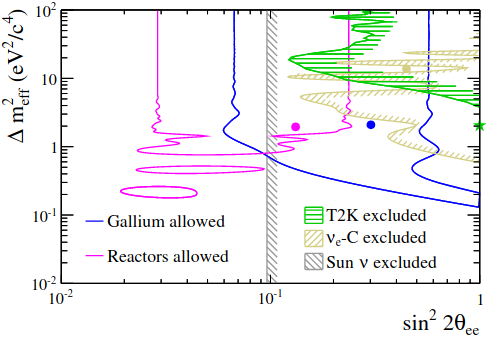
\includegraphics[width = 0.49\textwidth, height = 0.35\textwidth]{figures-chap6/external_limits/nue_dissap_external_combo.png}
    \caption[\nue disappearance limits from gallium and reactor experiments, the near detector of the  \gls{t2k} experiment and from \nue-carbon interaction data and solar neutrino data.]{Left: \nue disappearance exclusion and allowed regions from the near detector of the \gls{t2k} experiment. Right: \nue disappearance allowed regions from gallium and reactor experiments and exclusion regions from \gls{t2k}, \nue-carbon interaction data and solar neutrino data.}
    \label{fig:nue_disapp_external}
\end{figure}

\newpage
The remainder of this chapter will focus on the \nue channels. Some of the key results for the \numu channel are shown in \AppendixRef{app:numu_disapp} and a detailed discussion can be found in \cite{Rhiannon's_thesis}.


\newpage
\section{Systematic Uncertainties within SBN}

The systematics that are considered as part of the current \gls{sbn} analysis have been detailed in \SectionRef{sec:syst_uncertainties}. Unless explicitly stated, efficiency uncertainties are not considered due to there currently not being a general consensus on their magnitude. 

The systematics from the \gls{genie} and \gls{microboone} reweight packages are initially in the form of weights which correspond to variations of the parameter. Systematic uncertainties in this form can not be directly used in an oscillation analysis, but must instead first be processed internally, the details of which are described below.

\subsection{Processing Systematic Uncertainties}\label{sec:systematic_validation}

Many \textit{universes} are simulated, each with different weights associated with each of the systematic parameters. This allows the impact of varying systematic parameters on the event rate of neutrino interactions to be observed. If the systematic parameters are uncorrelated, the weights are simply an $n \sigma$ variation which is the value used in a given universe. For correlated parameters, the weights are due to a unique variation of all the correlated parameters of a given universe. Of the systematic uncertainties associated with either the \gls{genie} or \gls{microboone} reweight packages, only the neutrino production flux uncertainties which are listed in \TableRef{table:corr_flux} are correlated. All other parameters are uncorrelated. 

Depending on whether a given systematic parameter is correlated or not, the way that it is processed within VALOR is done in two different ways. For the uncorrelated parameters, a set of associated response functions which represent the impact on the event rate that tweaking a given systematic parameter will have are constructed. For each parameter, individual response functions are constructed for each combination of \textit{d, b, s, m, r} and \textit{t}. Each response function is a 13-knot spline which nominally represents the change in event rate from parameter variations ranging from \mbox{[-3, +3]$\sigma$} in 0.5$\sigma$ intervals. The response functions are constructed by first identifying the 12 universes which have a variation closest to each of the non-zero $\sigma$ intervals and then taking the ratio of the event rate from the selected universe in a \mbox{2D (r, t)} bin to the nominal event rate in that bin. By definition there will be a knot at 0$\sigma$ with a response of 1, however, in most cases, the remaining 12 knots will not be exactly at 0.5$\sigma$ intervals. 

For the case of correlated parameters, it is not straightforward to construct response functions as was done for the uncorrelated parameters because any variations will be due to multiple parameters. These parameters are instead represented by a covariance matrix. Matrices of this type, $\mathbf{C_{ij}}$, are constructed such that,
\begin{equation}
  \mathbf{C_{ij}} = \frac{1}{U} \sum_{u=1}^{U} (N_{i}^{u}-N_{i}^{cv})(N_{j}^{u}-N_{j}^{cv}),
  \label{eq:covmatrix}
\end{equation}
where \textit{U} is the number of universes, $N_{i,j}^{u}$ is the event rate in universe $u$ in bin $i$ or $j$ and $N_{i,j}^{cv}$ nominal event rate in
bin $i$ or $j$.

\subsection{Validating Systematic Uncertainties}
In order to establish that the systematic parameters are being correctly handled within VALOR, a comparison between the event rate variations as seen by VALOR and those obtained directly from the universes is performed. This is done in two different ways; 
\begin{enumerate}
    \item Tweak the nominal spectra using the response functions within VALOR for a single systematic parameter and then compare them with the spectra that were obtained directly from the universe files.
    \item Generate N toy samples (typically 500 in order to match the total number of universes) with some set of systematic parameters randomly tweaked. The one sigma spread from all the toys is found. This is done for both VALOR and for the universe files and the results are compared. 
\end{enumerate}

As an example, the $+1\sigma$ variation for the $f_{HornCurrent}$, $f_{M_A^{CCRes}}$ and $f_{\Delta \rightarrow N \gamma}$ parameters from the \nue sample in \gls{sbnd} between the VALOR response functions and the universes are shown in \FigureRef{fig:+1sigma_variations}\footnote{The terms \textit{spline} and \textit{response function} are used interchangeably.}. A complete list of the $+3\sigma$ variation comparisons for all the uncorrelated systematic parameters in \gls{sbnd} are shown for the \nue channel in \AppendixRef{app:single_parameter_variations}. In all cases, there is either perfect agreement or differences of only up to a few tens of events. It should be noted that the event rate shown in the spectra used for validating the systematic parameters for the \nue channel is several orders of magnitude greater than the nominal event rates as seen in for example \FigureRef{fig:nominal_nue_spectra}. This is due to manually setting the oscillation parameters to $\sin^2{2\theta_{\mu e}} = 1$ and $\Delta m_{41}^2 = 100$ eV$^2$ which ensures that many of the events from the oscillated $\numu \rightarrow \nue$ sub-sample are processed which is required because the response functions are indexed by mode and therefore contributions from all the sub-samples are needed. Since oscillation and systematic effects commute, this approach is sufficient to correctly produce a complete set of response functions. In the nominal event rate spectra, the assumption is that no oscillations occur, so no events from the oscillated sample are included hence the much lower event rate. 

\begin{figure}[h!]
    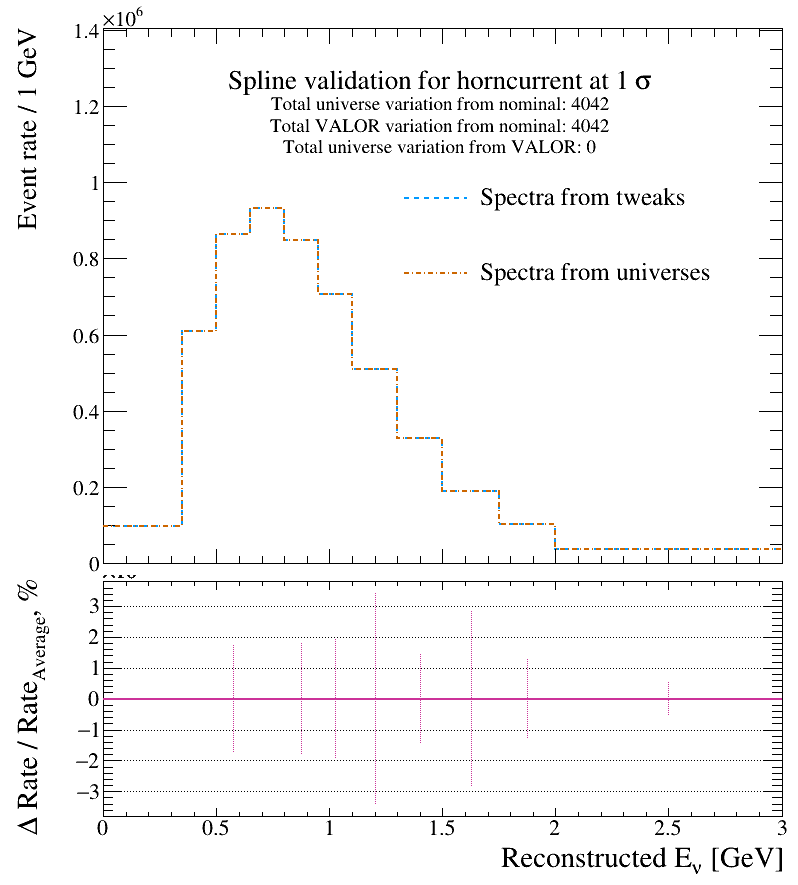
\includegraphics[width = 0.49\textwidth, height = 0.56184\textwidth]{figures-chap6/tweak_nsigma_nue/horncurrent_FluxUnisim_nuelikeCChigh_1sigma_horncurrent_FluxUnisim.png}
    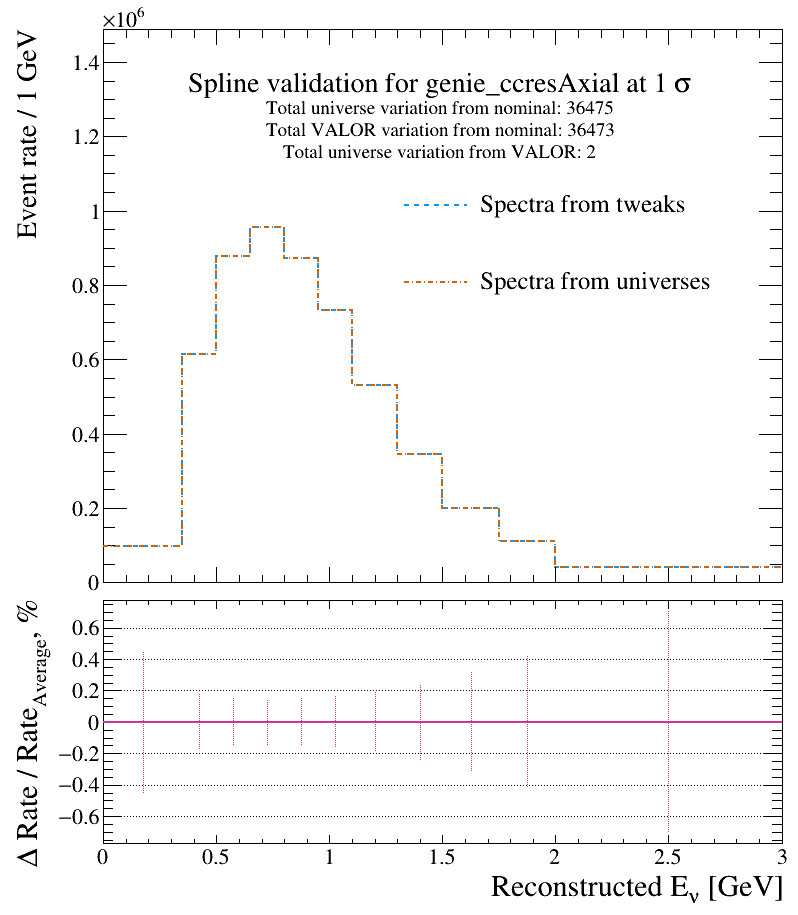
\includegraphics[width = 0.49\textwidth]{figures-chap6/tweak_nsigma_nue/genie_ccresAxial_Genie_nuelikeCChigh_1sigma_genie_ccresAxial_Genie.png}
    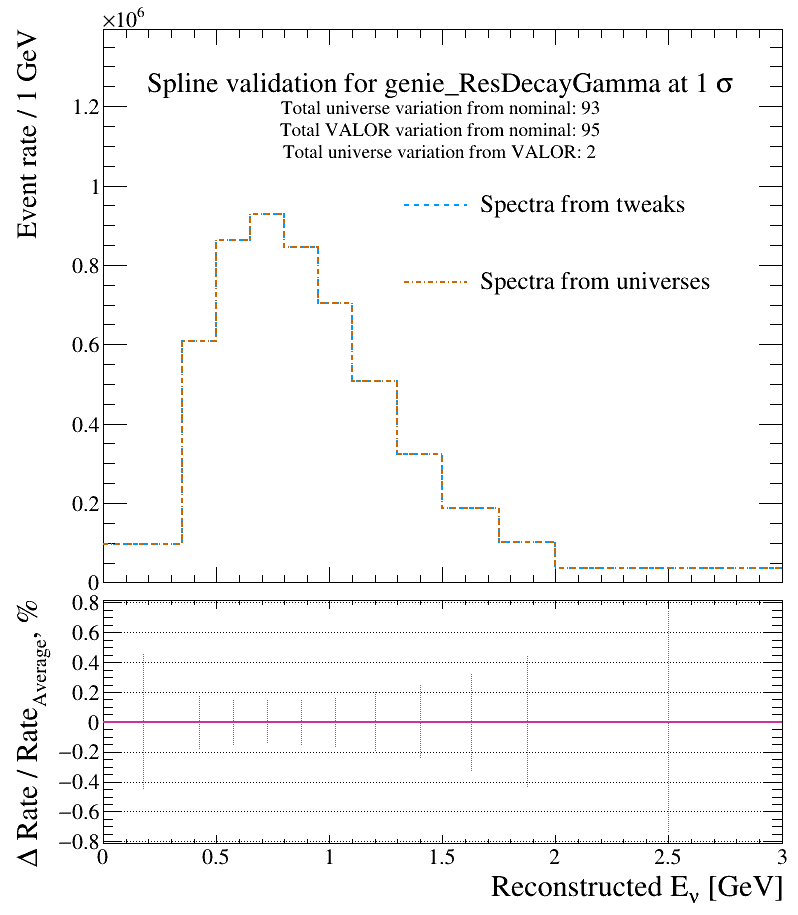
\includegraphics[width = 0.49\textwidth]{figures-chap6/tweak_nsigma_nue/genie_ResDecayGamma_Genie_nuelikeCChigh_1sigma_genie_ResDecayGamma_Genie.png}
  \captionsetup{width=0.49\textwidth}
  \parbox[b]{0.49\textwidth}%
  {
   \caption[+1$\sigma$ variation comparison for the $f_{HornCurrent}$, $f_{M_A^{CCRes}}$ and $f_{\Delta \rightarrow N \gamma}$ parameters.]{A comparison of the +1$\sigma$ variation from the response functions in VALOR and the universes for the $f_{HornCurrent}$, $f_{M_A^{CCRes}}$ and $f_{\Delta \rightarrow N \gamma}$ parameters. The $f_{HornCurrent}$ parameter shows perfect agreement between VALOR and the universes whereas both the $f_{M_A^{CCRes}}$ and $f_{\Delta \rightarrow N \gamma}$ parameters only have an event rate difference of 2. \\\phantom{.}\\
   \label{fig:+1sigma_variations}}
   }
\end{figure}

\FigureRef{fig:1sigma_variations_toys} shows a double ratio comparison from VALOR and the universes for the flux, proposal interaction and modern interaction systematic parameters. These plots are constructed by first finding the ratio between the 1$\sigma$ variation and the nominal using VALOR and the analogous ratio using the universe files. The double ratio is then constructed by taking the ratio of both the previous 1$\sigma$ ratios. There are some minor differences between the variations in VALOR and the universes, however, event-perfect agreement is not expected since the 1$\sigma$ variations are found by taking the average from many toy samples. Nevertheless, the disagreement is for the most part $< 1\%$ with a maximum of just over 2\%. 



\begin{figure}[h!]
    \begin{comment}
    Was too lazy to remake the plots and remove the label so have just overlayed a white box to hide.
    \end{comment}
    \begin{tikzpicture}
    \node at (0,0) {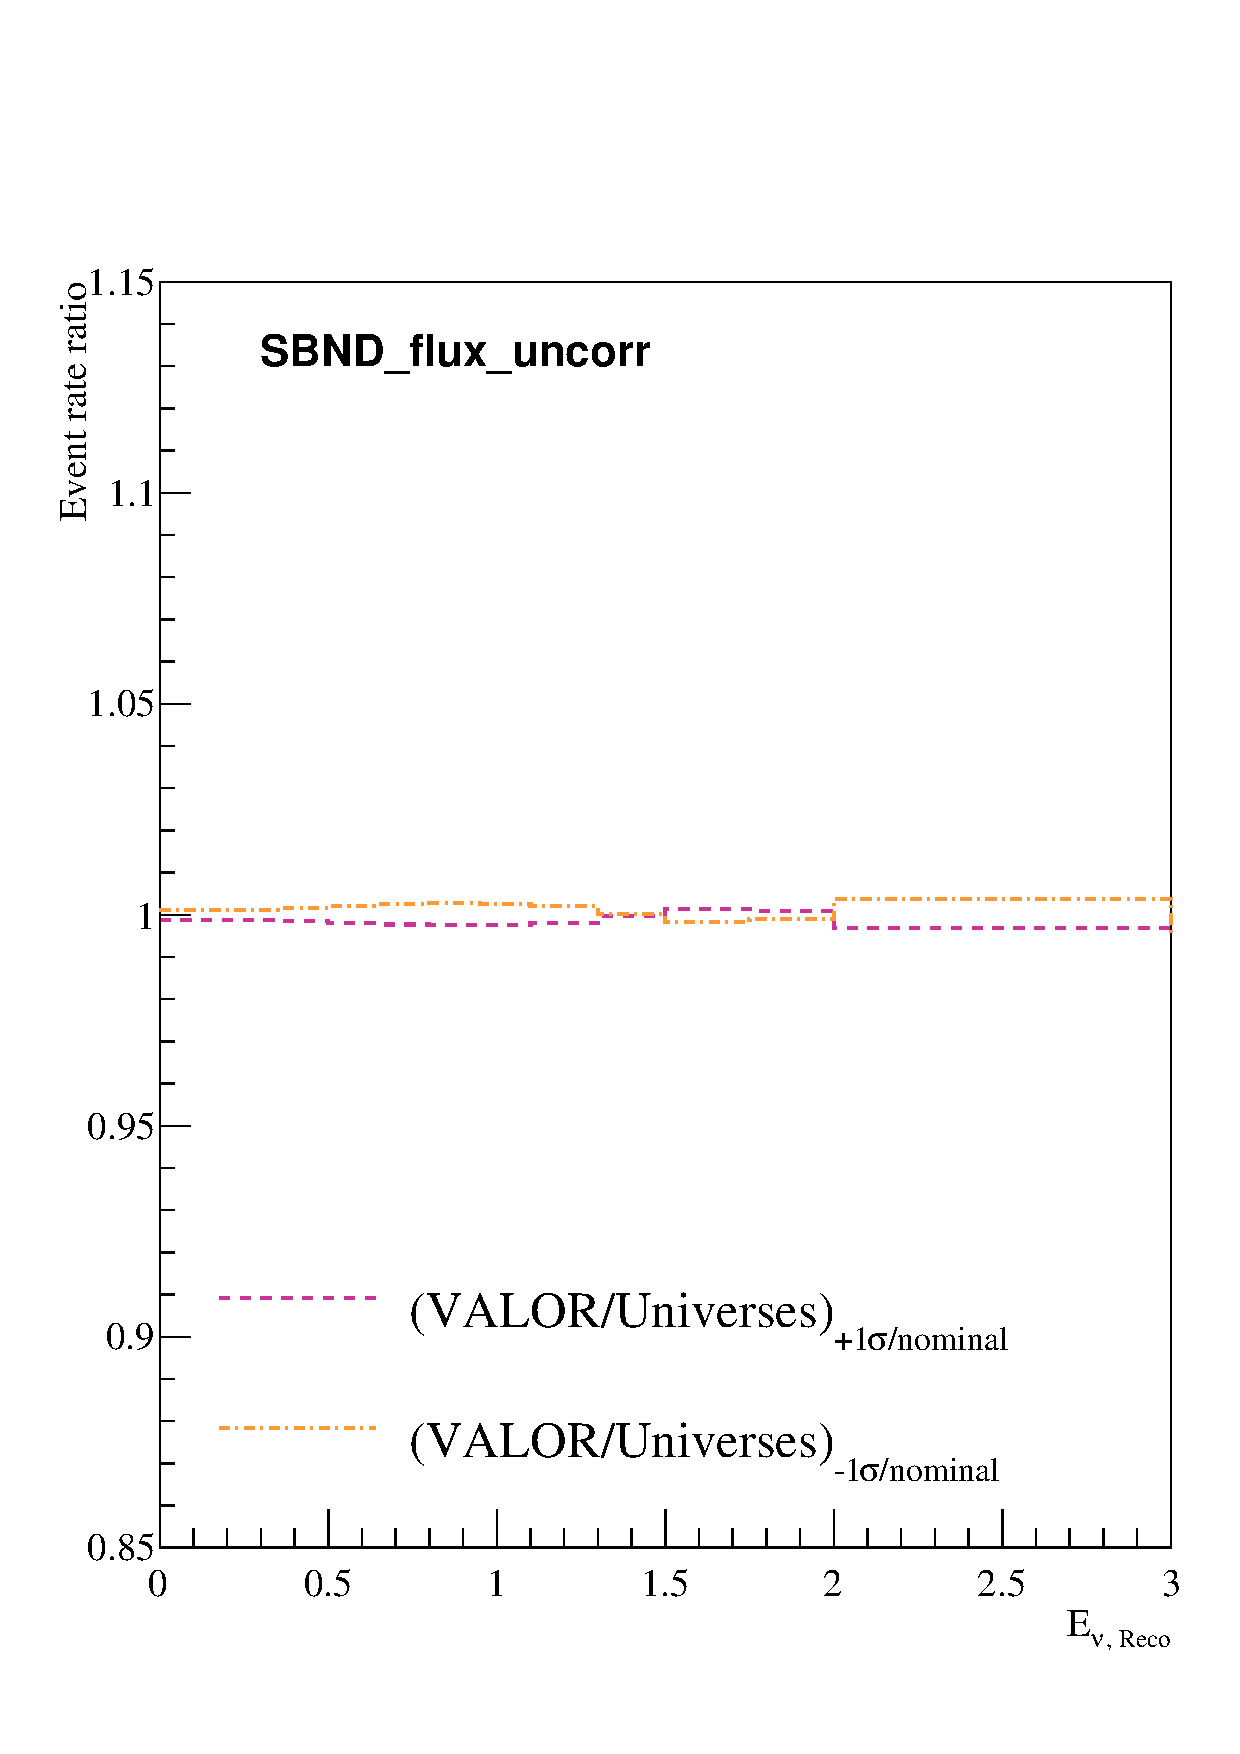
\includegraphics[width = 0.45\textwidth, height = 0.56184\textwidth]{figures-chap6/tweak_pdf_N_nue/universe_valor_double_ratios_SBND_flux_uncorr.pdf}};
    \draw [fill=white, draw=white] (-2.5,3)--(1,3)--(1,3.5)--(-2.5,3.5)--cycle;
    \end{tikzpicture}
    %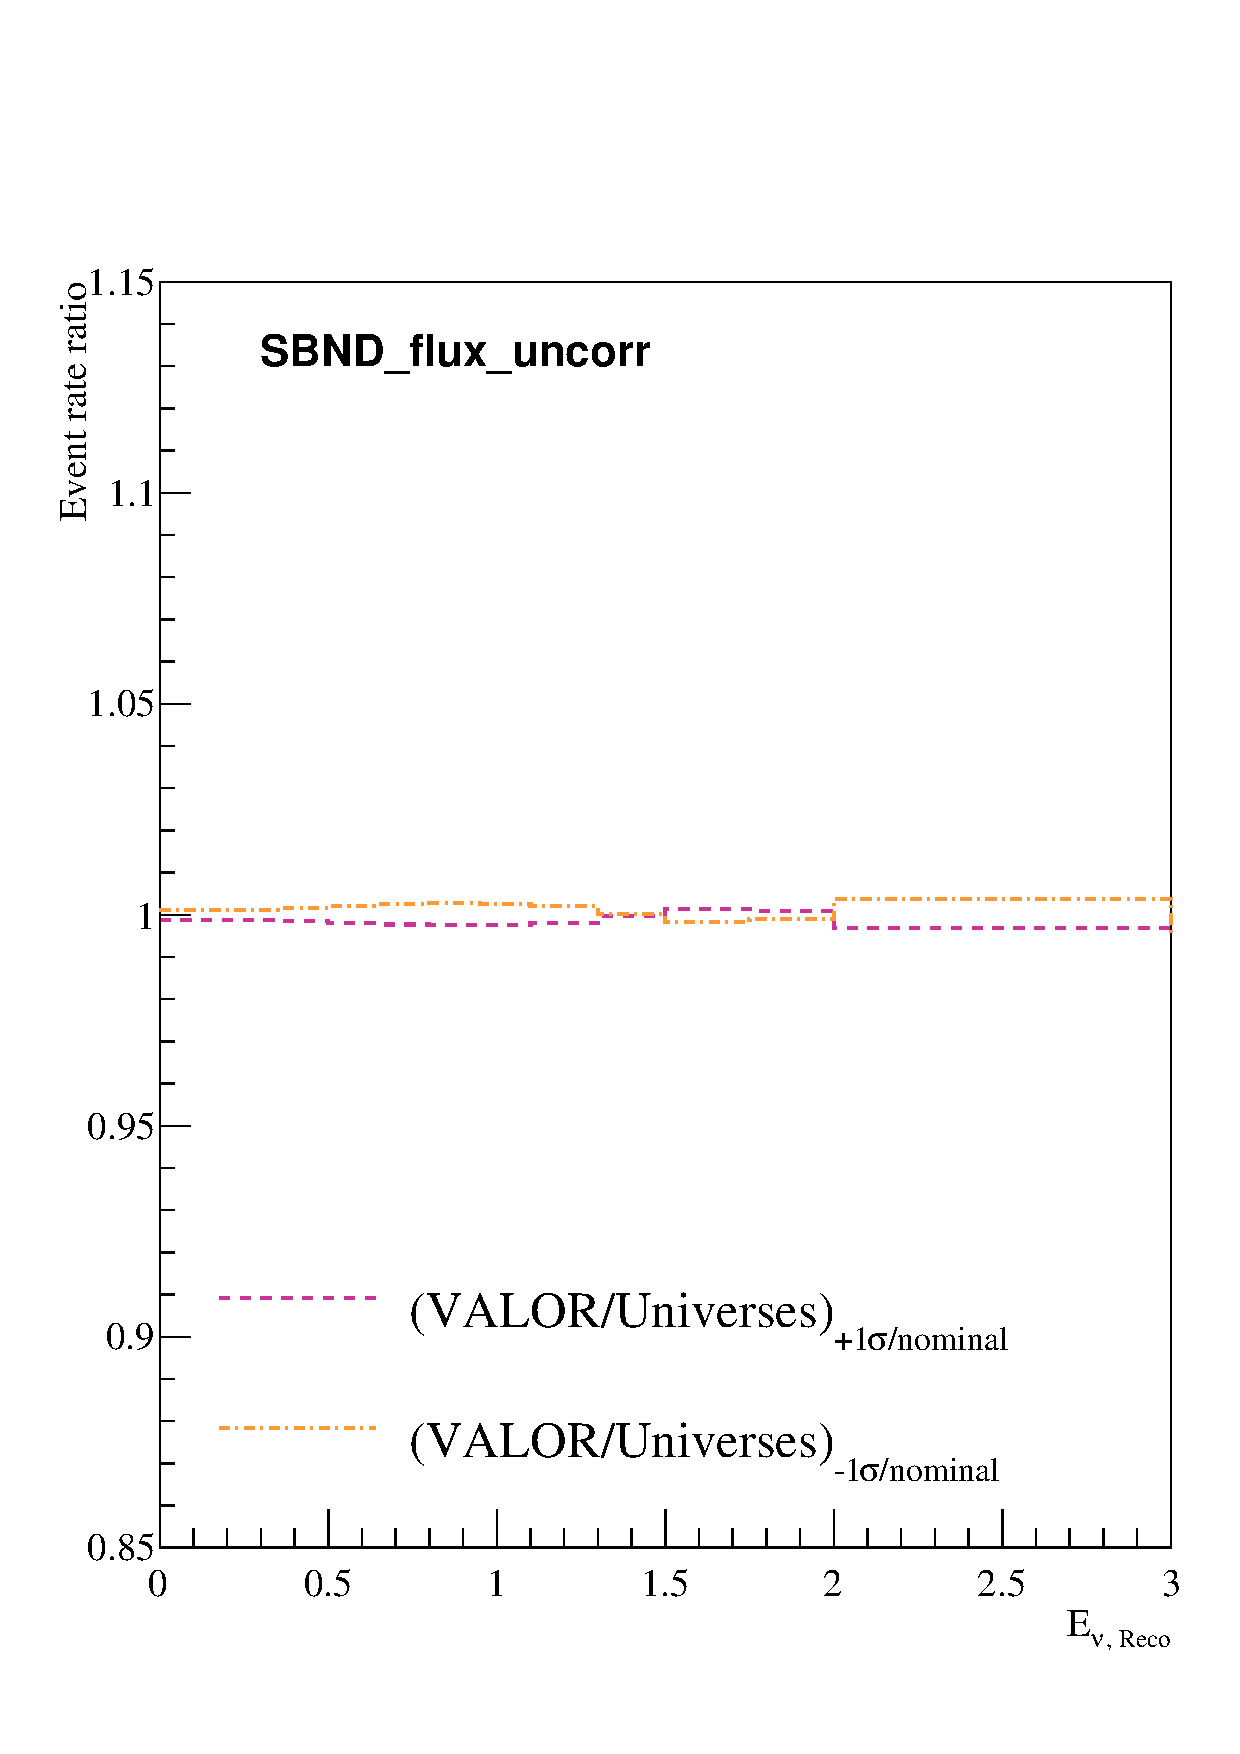
\includegraphics[width = 0.49\textwidth, height = 0.56184\textwidth]{figures-chap6/tweak_pdf_N_nue/universe_valor_double_ratios_SBND_flux_uncorr.pdf}
    \begin{tikzpicture}
    \node at (0,0) {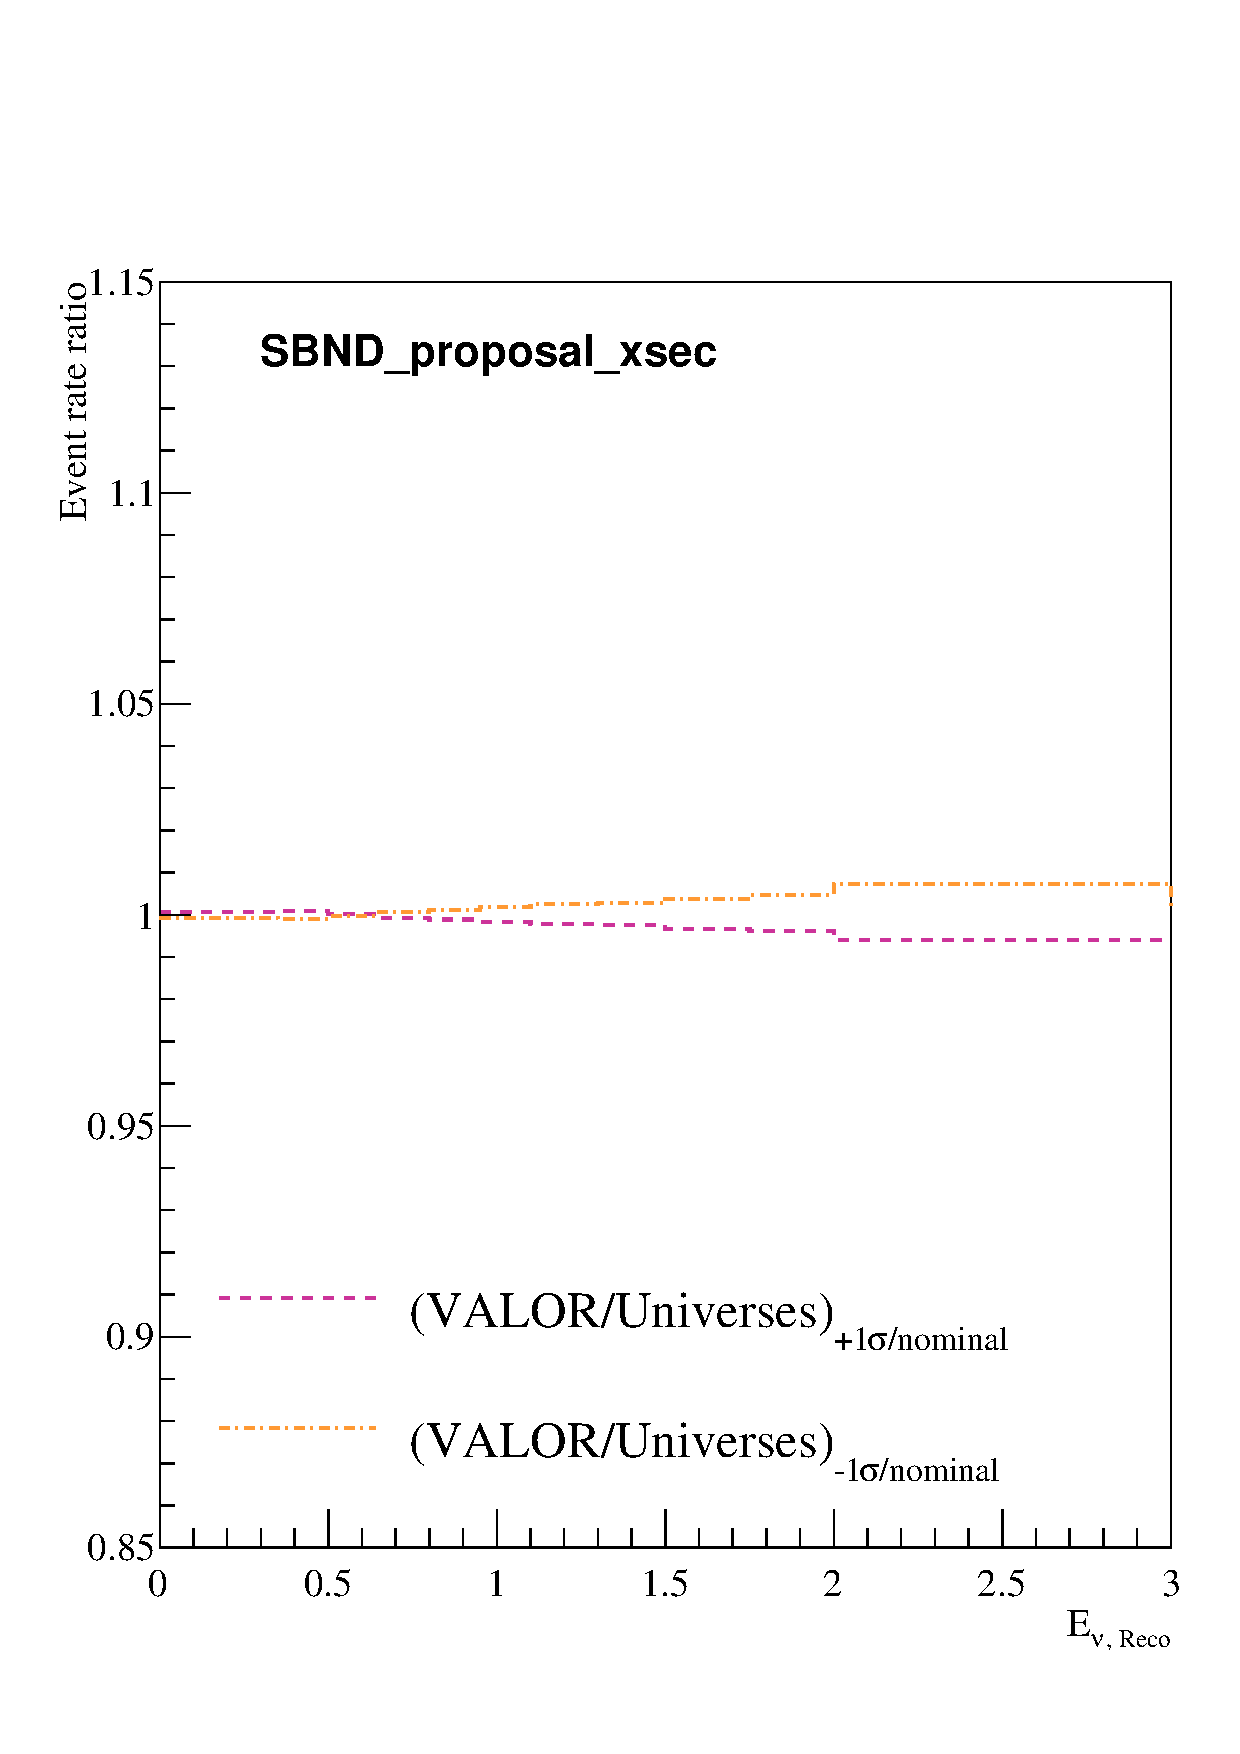
\includegraphics[width = 0.45\textwidth, height = 0.56184\textwidth]{figures-chap6/tweak_pdf_N_nue/universe_valor_double_ratios_SBND_proposal_xsec.pdf}};
     \draw [fill=white, draw=white] (-2.5,3)--(1,3)--(1,3.5)--(-2.5,3.5)--cycle;
    \end{tikzpicture}
    \begin{tikzpicture}
    \node at (0,0) {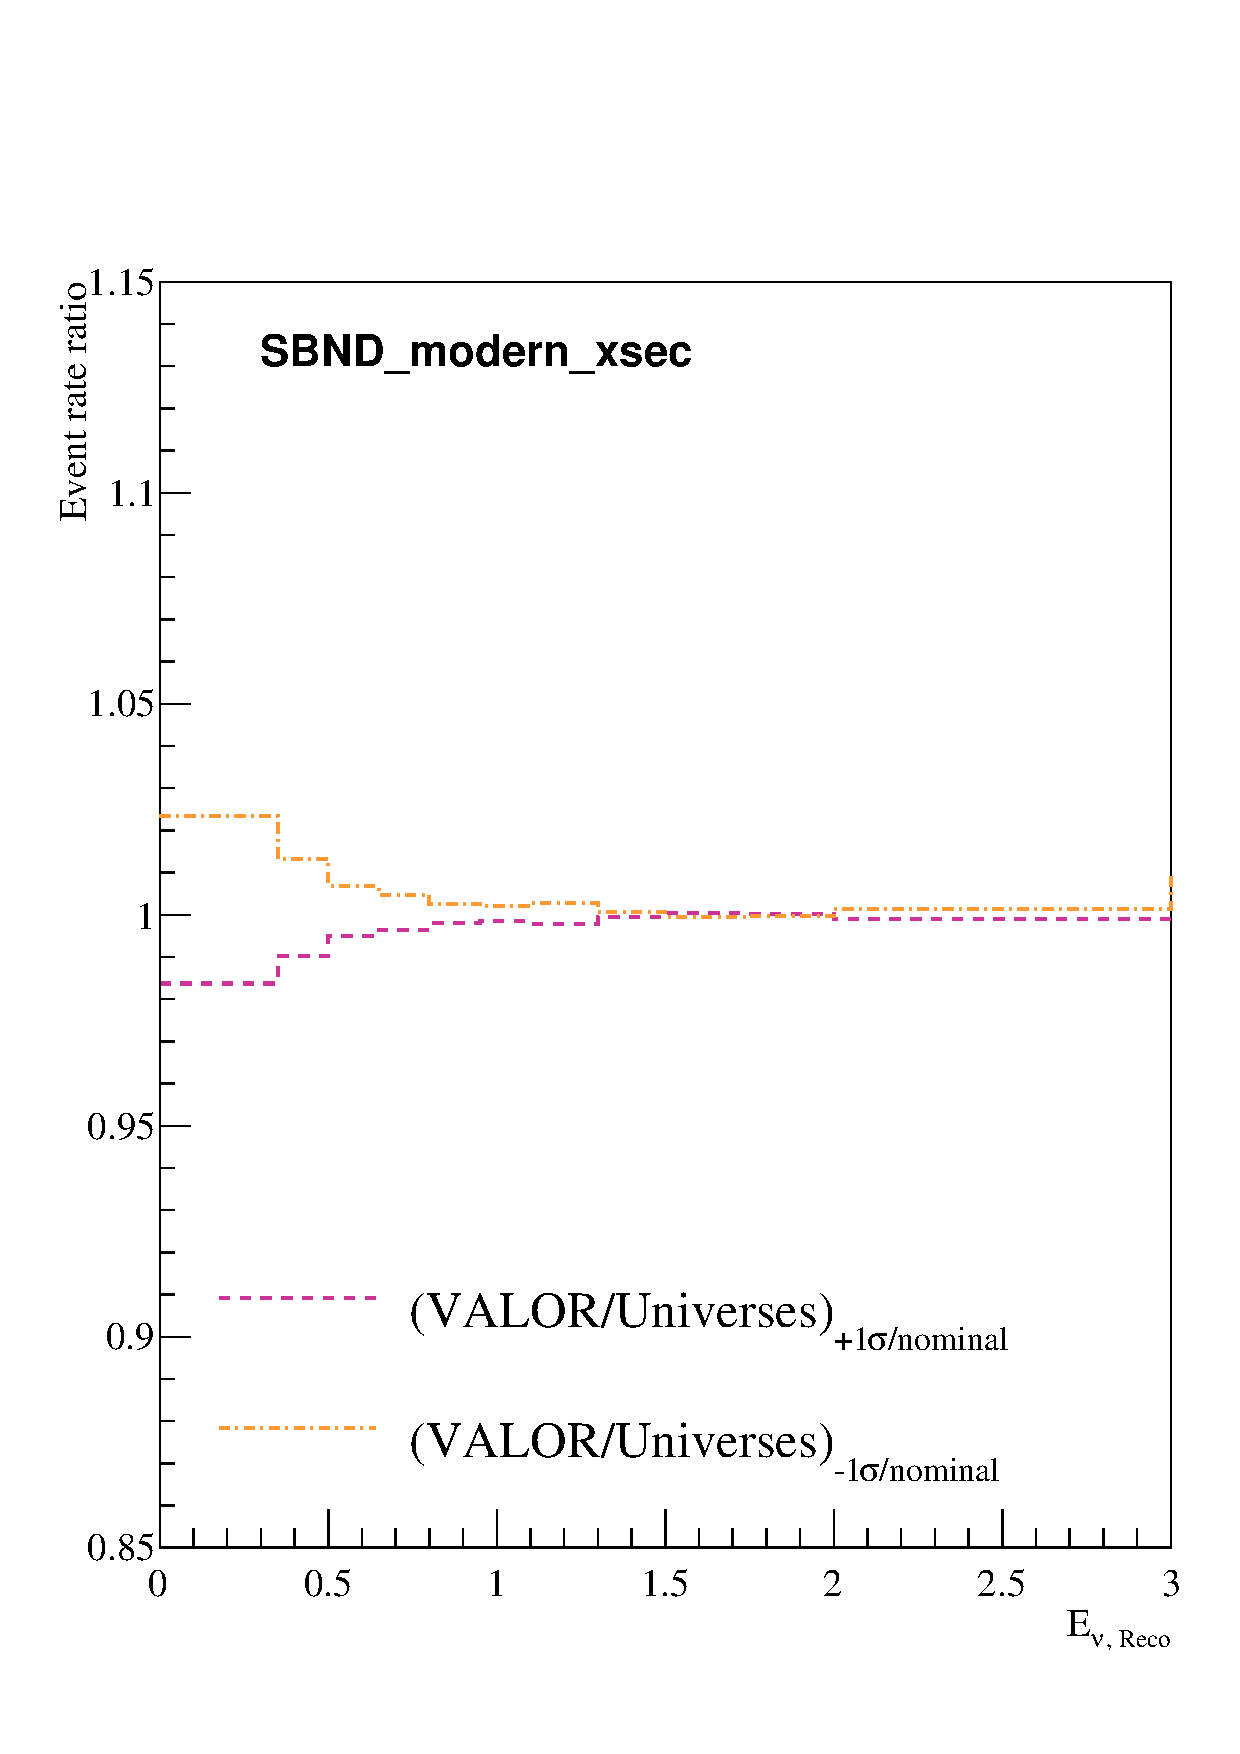
\includegraphics[width = 0.45\textwidth, height = 0.56184\textwidth]{figures-chap6/tweak_pdf_N_nue/universe_valor_double_ratios_SBND_modern_xsec.pdf}};
     \draw [fill=white, draw=white] (-2.5,3)--(1,3)--(1,3.5)--(-2.5,3.5)--cycle;
    \end{tikzpicture}
    \vspace{0.1\textwidth}
  \captionsetup{width=0.45\textwidth}
  \parbox[b]{0.45\textwidth}%
  {
   \caption[The ratio between the $\pm 1 \sigma$ variation from VALOR. and the universes for the flux, proposal interaction and modern interaction set of systematics.]{The ratio between the $\pm 1 \sigma$ variation from VALOR and the universes for the flux, proposal interaction and modern interaction set of systematic parameters.  \\\phantom{.}\\\phantom{.}\\\phantom{.}\\
   \label{fig:1sigma_variations_toys}}
  }
\end{figure}

\clearpage

\section{Event Rate Predictions and the Expected Signal}
\begin{comment}
Event rates
Impact of systematics
Size of Signal
\end{comment}

In order to perform sensitivity calculations, the events are required to be binned in terms of a kinematical variable, which is chosen to be the neutrino energy.

The nominal event rates, event rates with an uncertainty envelope due to systematic uncertainties and the event rates due to an oscillation signal are discussed below for each \gls{sbn} detector. Additionally, the impact of the uncorrelated systematic parameters are quantified in terms of their effect on the oscillation parameters.


\subsection{Nominal Event Rate Predictions}

It has been established that there are two oscillations channels associated with \nue: \nue appearance and \nue disappearance. Since the only difference between these channels is due to oscillations, the nominal event rates are common between the two.

The breakdown of the nominal number of events by interaction mode and channel are shown numerically in \TableRef{table:sbnd_nue_event_rate}, \TableRef{table:uboone_nue_event_rate} and \TableRef{table:icarus_nue_event_rate} for \gls{sbnd}, \gls{microboone} and \gls{icarus} respectively. The same events rates are also shown in \FigureRef{fig:nominal_nue_spectra} in the form of spectra. The spectra show the modal breakdown in terms of the coarse reaction modes where the events have been binned in reconstructed neutrino energy. 

Similar to \FigureRef{fig:nominal_nue_spectra}, \FigureRef{fig:nominal_nue_spectra_1sigma_enevelope} again shows the nominal event rate in each \gls{sbn} detector, but in an integrated form. Additionally, $1\sigma$ prefit uncertainty envelopes are shown which are due to the flux and interaction systematics. The accuracy of say the \gls{icarus} prediction can be improved by constraining the systematics from an \gls{sbnd} fit. This is shown in \FigureRef{fig:icarus_pre_post_fit} which shows the nominal integrated \gls{icarus} spectrum along with the prefit uncertainty envelope as in \FigureRef{fig:nominal_nue_spectra_1sigma_enevelope}, but also a postfit uncertainty envelope based on an \gls{sbnd} fit is shown. The reduction in size from the prefit to postfit envelope highlights the impact of \gls{sbnd} on the \gls{icarus} prediction. 

\newpage
\begin{table}
%\section*{sbn\_nd\_\_BNB\_FHC\_\_nuelikeCChigh}
\begin{adjustbox}{width=1\textwidth}
\begin{tabular} {  l r  r  r  r  r  r  r  r  }
\hline
              & $\nu_{\mu} \rightarrow \nu_{\mu}$ & $\bar{\nu}_{\mu} \rightarrow \bar{\nu}_{\mu}$ & $\nu_{e} \rightarrow \nu_{e}$ & $\bar{\nu}_{e} \rightarrow \bar{\nu}_{e}$ & $\nu_{\mu} \rightarrow \nu_{e}$ & $\bar{\nu}_{\mu} \rightarrow \bar{\nu}_{e}$ & Non-neutrino         & Total                \\ \hline\hline
 CCQE         & 17.0                 & 0.0                  & 5957.8               & 166.6                & 0.0                  & 0.0                  & N/A                  & 6141.5               \\ \hline
 CCMEC        & 1.1                  & 0.0                  & 1433.0               & 59.7                 & 0.0                  & 0.0                  & N/A                  & 1493.8               \\ \hline
 CC1$\pi^{\pm}$ & 234.6                & 0.0                  & 2859.9               & 112.4                & 0.0                  & 0.0                  & N/A                  & 3206.8               \\ \hline
 CC1$\pi^{0}$   & 230.7                & 0.0                  & 513.8                & 14.6                 & 0.0                  & 0.0                  & N/A                  & 759.2                \\ \hline
 CC2$\pi^{\pm}$ & 19.3                 & 0.0                  & 293.3                & 7.9                  & 0.0                  & 0.0                  & N/A                  & 320.6                \\ \hline
 CC2$\pi^{0}$   & 5.2                  & 0.0                  & 24.1                 & 0.6                  & 0.0                  & 0.0                  & N/A                  & 29.9                 \\ \hline
 CC1$\pi^{0}1\pi^{\pm}$ & 37.1                 & 0.0                  & 187.0                & 7.0                  & 0.0                  & 0.0                  & N/A                  & 231.1                \\ \hline
 CCcoherent   & 0.0                  & 0.0                  & 38.1                 & 3.8                  & 0.0                  & 0.0                  & N/A                  & 41.9                 \\ \hline
 CC\nue\text{El} & 0.0                  & 0.0                  & N/A                  & N/A                  & N/A                  & N/A                  & N/A                  & 0.0                  \\ \hline
 CCother      & 20.7                 & 0.0                  & 270.9                & 8.3                  & 0.0                  & 0.0                  & N/A                  & 299.9                \\ \hline
 NCEL         & 3.4                  & 0.0                  & 0.0                  & 0.0                  & N/A                  & N/A                  & N/A                  & 3.5                  \\ \hline
 NCMEC        & 0.6                  & 0.0                  & 0.0                  & 0.0                  & N/A                  & N/A                  & N/A                  & 0.6                  \\ \hline
 NC1$\pi^{\pm}$ & 135.6                & 0.0                  & 0.8                  & 0.0                  & N/A                  & N/A                  & N/A                  & 136.4                \\ \hline
 NC1$\pi^{0}$   & 772.6                & 0.0                  & 5.5                  & 0.2                  & N/A                  & N/A                  & N/A                  & 778.4                \\ \hline
 NC2$\pi^{\pm}$ & 2.3                  & 0.0                  & 0.1                  & 0.0                  & N/A                  & N/A                  & N/A                  & 2.4                  \\ \hline
 NC2$\pi^{0}$   & 6.9                  & 0.0                  & 0.1                  & 0.0                  & N/A                  & N/A                  & N/A                  & 7.0                  \\ \hline
 NC1$\pi^{0}1\pi^{\pm}$ & 16.1                 & 0.0                  & 0.4                  & 0.0                  & N/A                  & N/A                  & N/A                  & 16.5                 \\ \hline
 NCcoherent   & 76.8                 & 0.0                  & 0.4                  & 0.1                  & N/A                  & N/A                  & N/A                  & 77.2                 \\ \hline
 NC1$\gamma$    & 0.0                  & 0.0                  & 0.0                  & 0.0                  & N/A                  & N/A                  & N/A                  & 0.0                  \\ \hline
 NC\nue\text{El} & 181.9                & 0.0                  & N/A                  & N/A                  & N/A                  & N/A                  & N/A                  & 181.9                \\ \hline
 NCother      & 50.0                 & 0.0                  & 0.5                  & 0.0                  & N/A                  & N/A                  & N/A                  & 50.5                 \\ \hline
 \nue\text{El} & N/A                  & N/A                  & 0.0                  & 0.0                  & 0.0                  & 0.0                  & N/A                  & 0.0                  \\ \hline
 cosmic       & N/A                  & N/A                  & N/A                  & N/A                  & N/A                  & N/A                  & 0.3                  & 0.3                  \\ \hline
 dirt         & N/A                  & N/A                  & N/A                  & N/A                  & N/A                  & N/A                  & 33.9                 & 33.9                 \\ \hline
\hline
 Total        & 1812.0               & 0.0                  & 11585.9              & 381.3                & 0.0                  & 0.0                  & 34.2                 & 13813.5              \\ \hline


\end{tabular}
\end{adjustbox}

%\noindent Total: 13813.452    (13813.452) \newline
%POT: 6.600E20
\caption[Nominal \nue event rate breakdown in \gls{sbnd}.]{Nominal \nue event rate breakdown in \gls{sbnd}.}
\label{table:sbnd_nue_event_rate}
\end{table}


\newpage
\begin{table}
%\section*{sbn\_uboone\_\_BNB\_FHC\_\_nuelikeCChigh}
\begin{adjustbox}{width=1\textwidth}
\begin{tabular} {l r r r r r r r r}
\hline

              & $\nu_{\mu} \rightarrow \nu_{\mu}$ & $\bar{\nu}_{\mu} \rightarrow \bar{\nu}_{\mu}$ & $\nu_{e} \rightarrow \nu_{e}$ & $\bar{\nu}_{e} \rightarrow \bar{\nu}_{e}$ & $\nu_{\mu} \rightarrow \nu_{e}$ & $\bar{\nu}_{\mu} \rightarrow \bar{\nu}_{e}$ & Non-neutrino         & Total                \\ \hline\hline
 CCQE         & 4.2                  & 0.0                  & 384.9                & 10.4                 & 0.0                  & 0.0                  & N/A                  & 399.5                \\ \hline
 CCMEC        & 0.1                  & 0.0                  & 93.9                 & 3.7                  & 0.0                  & 0.0                  & N/A                  & 97.6                 \\ \hline
 CC1$\pi^{\pm}$ & 18.9                 & 0.0                  & 196.8                & 7.5                  & 0.0                  & 0.0                  & N/A                  & 223.2                \\ \hline
 CC1$\pi^{0}$   & 19.1                 & 1.0                  & 35.5                 & 1.1                  & 0.0                  & 0.0                  & N/A                  & 56.7                 \\ \hline
 CC2$\pi^{\pm}$ & 1.0                  & 0.0                  & 21.9                 & 0.6                  & 0.0                  & 0.0                  & N/A                  & 23.5                 \\ \hline
 CC2$\pi^{0}$   & 3.3                  & 0.0                  & 1.9                  & 0.1                  & 0.0                  & 0.0                  & N/A                  & 5.2                  \\ \hline
 CC1$\pi^{0}1\pi^{\pm}$ & 7.2                  & 0.0                  & 13.6                 & 0.6                  & 0.0                  & 0.0                  & N/A                  & 21.4                 \\ \hline
 CCcoherent   & 0.0                  & 0.0                  & 2.6                  & 0.4                  & 0.0                  & 0.0                  & N/A                  & 3.0                  \\ \hline
 CC\nue\text{El} & 0.0                  & 0.0                  & N/A                  & N/A                  & N/A                  & N/A                  & N/A                  & 0.0                  \\ \hline
 CCother      & 3.3                  & 0.0                  & 19.1                 & 0.4                  & 0.0                  & 0.0                  & N/A                  & 22.9                 \\ \hline
 NCEL         & 0.3                  & 0.0                  & 0.0                  & 0.0                  & N/A                  & N/A                  & N/A                  & 0.3                  \\ \hline
 NCMEC        & 0.0                  & 0.0                  & 0.0                  & 0.0                  & N/A                  & N/A                  & N/A                  & 0.0                  \\ \hline
 NC1$\pi^{\pm}$ & 13.9                 & 0.0                  & 0.1                  & 0.0                  & N/A                  & N/A                  & N/A                  & 14.0                 \\ \hline
 NC1$\pi^{0}$   & 59.3                 & 1.0                  & 0.4                  & 0.0                  & N/A                  & N/A                  & N/A                  & 60.7                 \\ \hline
 NC2$\pi^{\pm}$ & 0.7                  & 0.0                  & 0.0                  & 0.0                  & N/A                  & N/A                  & N/A                  & 0.7                  \\ \hline
 NC2$\pi^{0}$   & 0.7                  & 0.1                  & 0.0                  & 0.0                  & N/A                  & N/A                  & N/A                  & 0.7                  \\ \hline
 NC1$\pi^{0}1\pi^{\pm}$ & 2.3                  & 0.0                  & 0.0                  & 0.0                  & N/A                  & N/A                  & N/A                  & 2.3                  \\ \hline
 NCcoherent   & 5.5                  & 0.2                  & 0.0                  & 0.0                  & N/A                  & N/A                  & N/A                  & 5.8                  \\ \hline
 NC1$\gamma$    & 0.0                  & 0.0                  & 0.0                  & 0.0                  & N/A                  & N/A                  & N/A                  & 0.0                  \\ \hline
 NC\nue\text{El} & 14.9                 & 0.0                  & N/A                  & N/A                  & N/A                  & N/A                  & N/A                  & 14.9                 \\ \hline
 NCother      & 3.3                  & 0.0                  & 0.0                  & 0.0                  & N/A                  & N/A                  & N/A                  & 3.3                  \\ \hline
 \nue\text{El} & N/A                  & N/A                  & 0.0                  & 0.0                  & 0.0                  & 0.0                  & N/A                  & 0.0                  \\ \hline
 cosmic       & N/A                  & N/A                  & N/A                  & N/A                  & N/A                  & N/A                  & 0.0                  & 0.0                  \\ \hline
 dirt         & N/A                  & N/A                  & N/A                  & N/A                  & N/A                  & N/A                  & 14.8                 & 14.8                 \\ \hline
\hline
Total        & 157.8                & 2.3                  & 770.9                & 24.8                 & 0.0                  & 0.0                  & 14.8                 & 970.6            

       \\ \hline

\end{tabular}
\end{adjustbox}

%\noindent Total: 970.564    (970.564) \newline
%POT: 13.200E20
\caption[Nominal \nue event rate breakdown in \gls{microboone}.]{Nominal \nue event rate breakdown in \gls{microboone}.}
\label{table:uboone_nue_event_rate}
\end{table}


\newpage
\begin{table}
%\section*{sbn\_icarus\_\_BNB\_FHC\_\_nuelikeCChigh}
\begin{adjustbox}{width=1\textwidth}
\begin{tabular} {l r r r r r r r r}
\hline

              & $\nu_{\mu} \rightarrow \nu_{\mu}$ & $\bar{\nu}_{\mu} \rightarrow \bar{\nu}_{\mu}$ & $\nu_{e} \rightarrow \nu_{e}$ & $\bar{\nu}_{e} \rightarrow \bar{\nu}_{e}$ & $\nu_{\mu} \rightarrow \nu_{e}$ & $\bar{\nu}_{\mu} \rightarrow \bar{\nu}_{e}$ & Non-neutrino         & Total                \\ \hline\hline
 CCQE         & 4.6                  & 0.0                  & 727.9                & 19.3                 & 0.0                  & 0.0                  & N/A                  & 751.9                \\ \hline
 CCMEC        & 0.2                  & 0.0                  & 176.5                & 7.1                  & 0.0                  & 0.0                  & N/A                  & 183.8                \\ \hline
 CC1$\pi^{\pm}$ & 37.4                 & 0.2                  & 372.3                & 12.9                 & 0.0                  & 0.0                  & N/A                  & 422.8                \\ \hline
 CC1$\pi^{0}$   & 25.8                 & 0.1                  & 64.8                 & 2.2                  & 0.0                  & 0.0                  & N/A                  & 92.9                 \\ \hline
 CC2$\pi^{\pm}$ & 4.9                  & 0.1                  & 39.4                 & 1.0                  & 0.0                  & 0.0                  & N/A                  & 45.4                 \\ \hline
 CC2$\pi^{0}$   & 2.9                  & 0.1                  & 3.6                  & 0.1                  & 0.0                  & 0.0                  & N/A                  & 6.6                  \\ \hline
 CC1$\pi^{0}1\pi^{\pm}$ & 7.5                  & 0.0                  & 25.8                 & 1.1                  & 0.0                  & 0.0                  & N/A                  & 34.5                 \\ \hline
 CCcoherent   & 0.0                  & 0.0                  & 5.0                  & 0.5                  & 0.0                  & 0.0                  & N/A                  & 5.4                  \\ \hline
 CC\nue\text{El} & 0.0                  & 0.0                  & N/A                  & N/A                  & N/A                  & N/A                  & N/A                  & 0.0                  \\ \hline
 CCother      & 2.8                  & 0.0                  & 36.9                 & 0.8                  & 0.0                  & 0.0                  & N/A                  & 40.5                 \\ \hline
 NCEL         & 0.5                  & 0.0                  & 0.0                  & 0.0                  & N/A                  & N/A                  & N/A                  & 0.5                  \\ \hline
 NCMEC        & 0.0                  & 0.0                  & 0.0                  & 0.0                  & N/A                  & N/A                  & N/A                  & 0.0                  \\ \hline
 NC1$\pi^{\pm}$ & 17.7                 & 0.2                  & 0.1                  & 0.0                  & N/A                  & N/A                  & N/A                  & 18.1                 \\ \hline
 NC1$\pi^{0}$   & 108.5                & 0.7                  & 0.7                  & 0.0                  & N/A                  & N/A                  & N/A                  & 110.0                \\ \hline
 NC2$\pi^{\pm}$ & 0.7                  & 0.0                  & 0.0                  & 0.0                  & N/A                  & N/A                  & N/A                  & 0.8                  \\ \hline
 NC2$\pi^{0}$   & 0.9                  & 0.0                  & 0.0                  & 0.0                  & N/A                  & N/A                  & N/A                  & 0.9                  \\ \hline
 NC1$\pi^{0}1\pi^{\pm}$ & 3.4                  & 0.1                  & 0.1                  & 0.0                  & N/A                  & N/A                  & N/A                  & 3.6                  \\ \hline
 NCcoherent   & 11.3                 & 0.4                  & 0.1                  & 0.0                  & N/A                  & N/A                  & N/A                  & 11.8                 \\ \hline
 NC1$\gamma$    & 0.0                  & 0.0                  & 0.0                  & 0.0                  & N/A                  & N/A                  & N/A                  & 0.0                  \\ \hline
 NC\nue\text{El} & 17.9                 & 0.0                  & N/A                  & N/A                  & N/A                  & N/A                  & N/A                  & 17.9                 \\ \hline
 NCother      & 8.0                  & 0.0                  & 0.1                  & 0.0                  & N/A                  & N/A                  & N/A                  & 8.1                  \\ \hline
 \nue\text{El} & N/A                  & N/A                  & 0.0                  & 0.0                  & 0.0                  & 0.0                  & N/A                  & 0.0                  \\ \hline
 cosmic       & N/A                  & N/A                  & N/A                  & N/A                  & N/A                  & N/A                  & 2.3                  & 2.3                  \\ \hline
 dirt         & N/A                  & N/A                  & N/A                  & N/A                  & N/A                  & N/A                  & 24.1                 & 24.1                 \\ \hline
\hline
 Total        & 255.0                & 2.0                  & 1453.3               & 44.9                 & 0.0                  & 0.0                  & 26.4                 & 1781.6       

 \\ \hline

\end{tabular}
\end{adjustbox}

%\noindent Total: 1781.637    (1781.637) \newline
%POT: 6.600E20
\caption[Nominal \nue event rate breakdown in \gls{icarus}.]{Nominal \nue event rate breakdown in \gls{icarus}.}
\label{table:icarus_nue_event_rate}
\end{table}

\begin{figure}[h!]
  {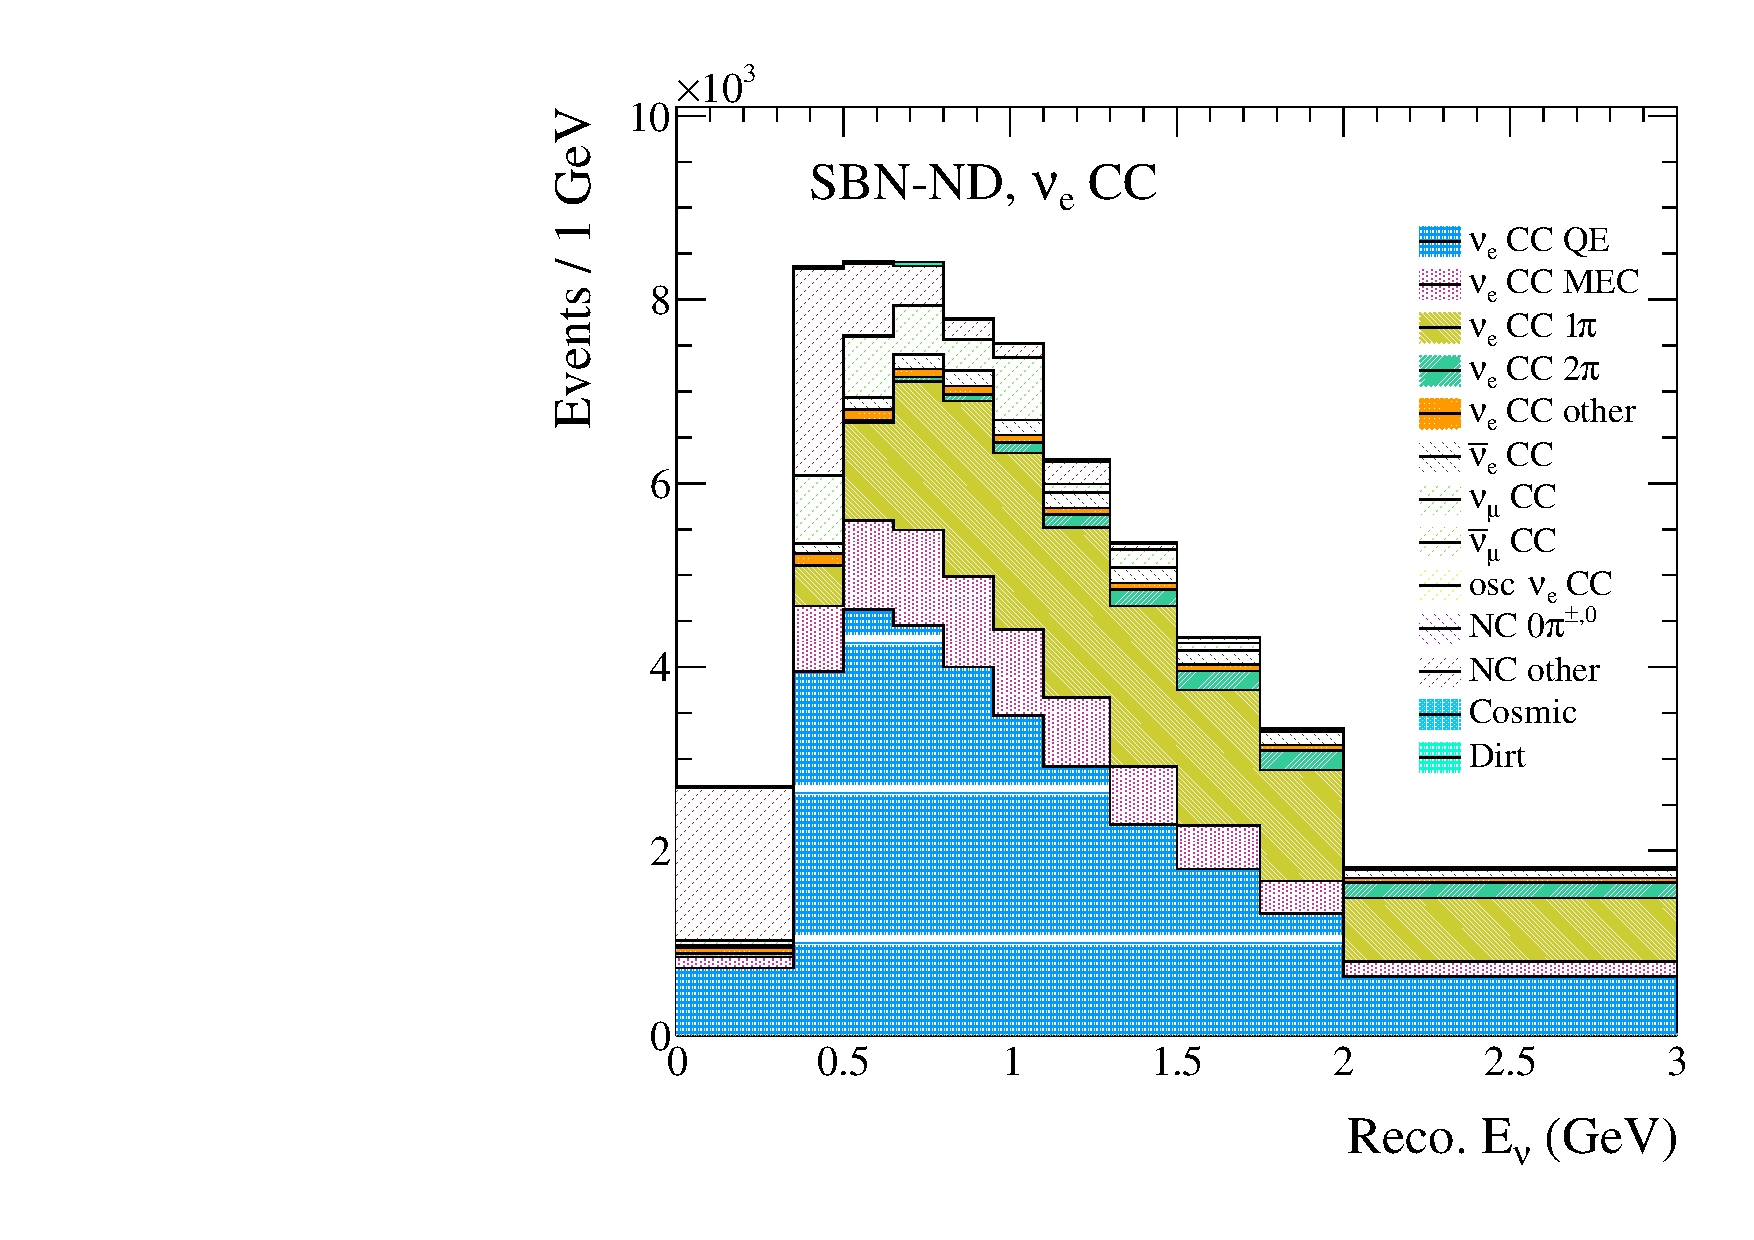
\includegraphics[width=0.49\textwidth]{figures-chap6/spectra/nue_nominal_spectrum_sbn_nd_BNB_FHC_0_modes.pdf}}
  {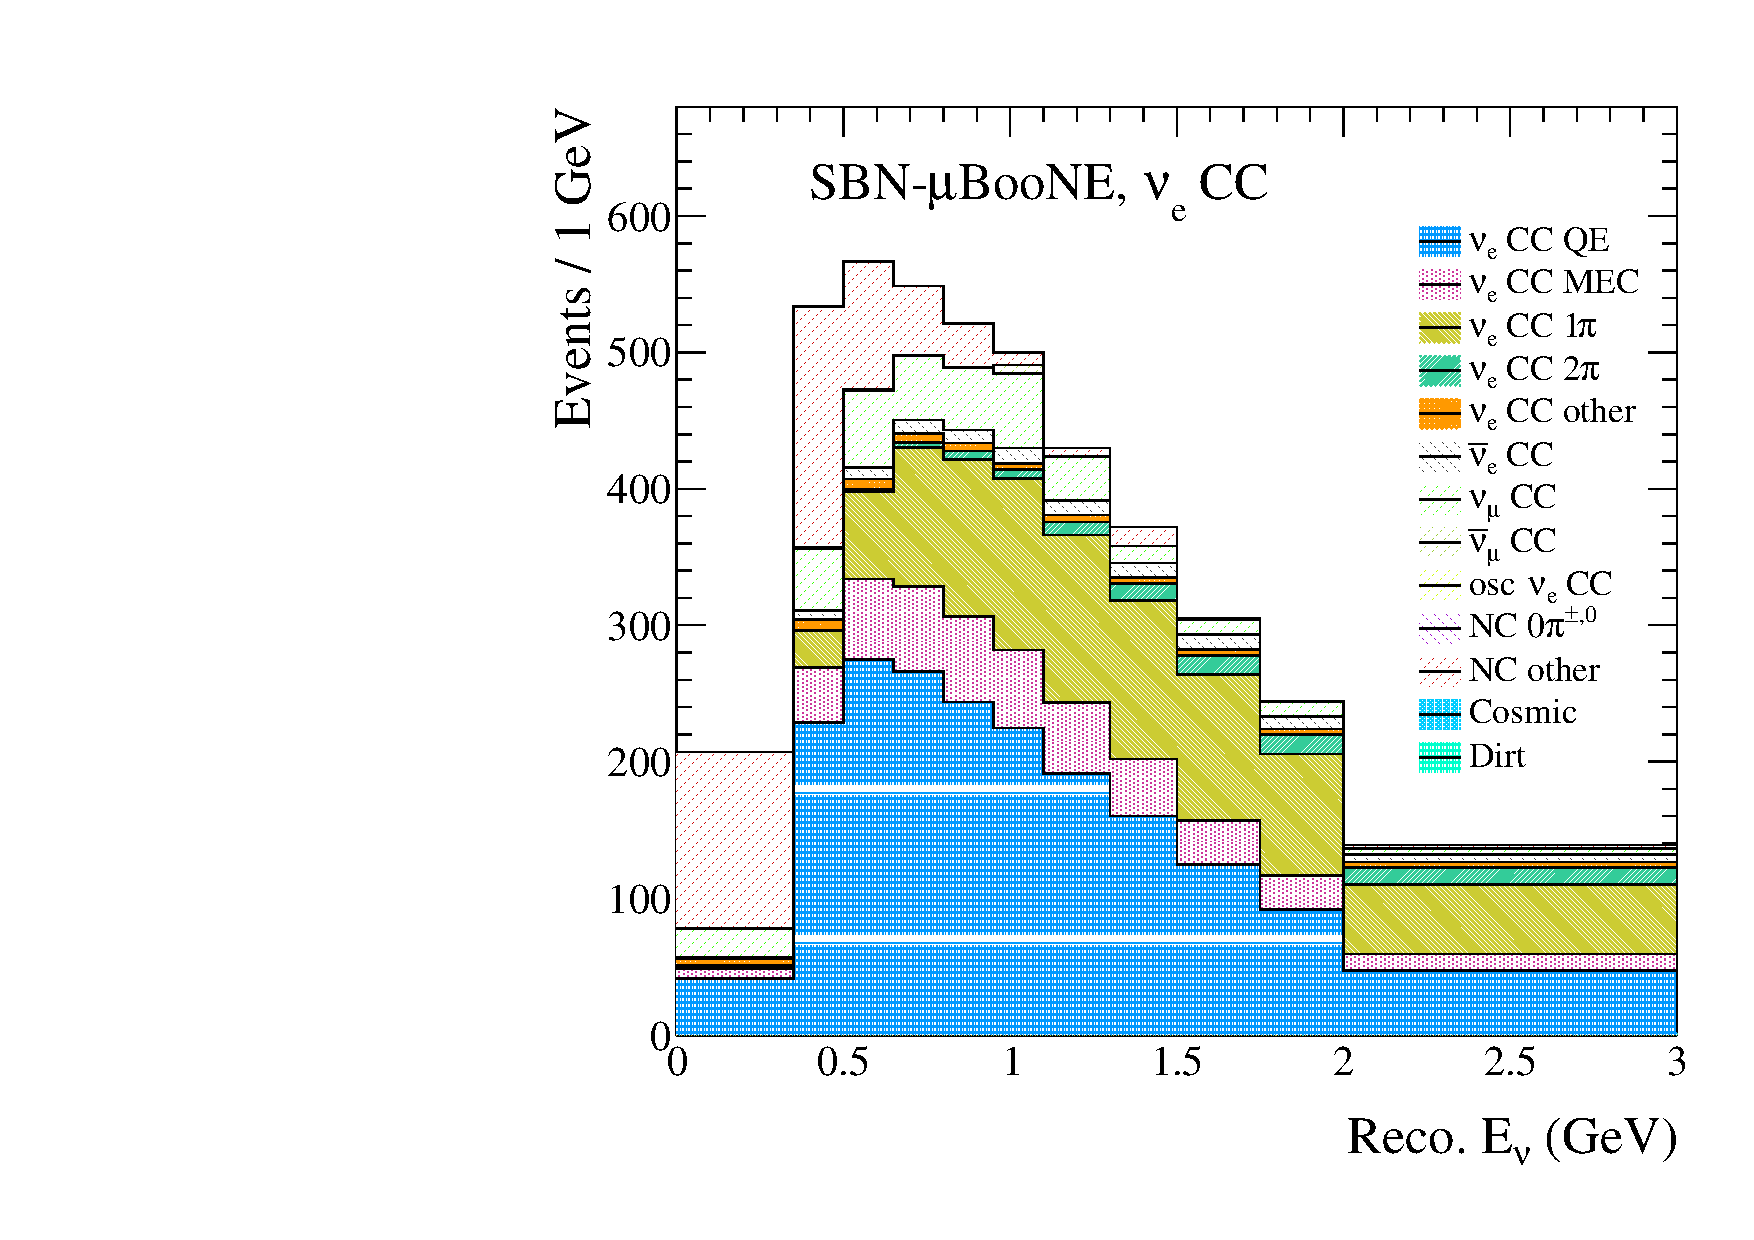
\includegraphics[width=0.49\textwidth]{figures-chap6/spectra/nue_nominal_spectrum_sbn_uboone_BNB_FHC_1_modes.pdf}}
  {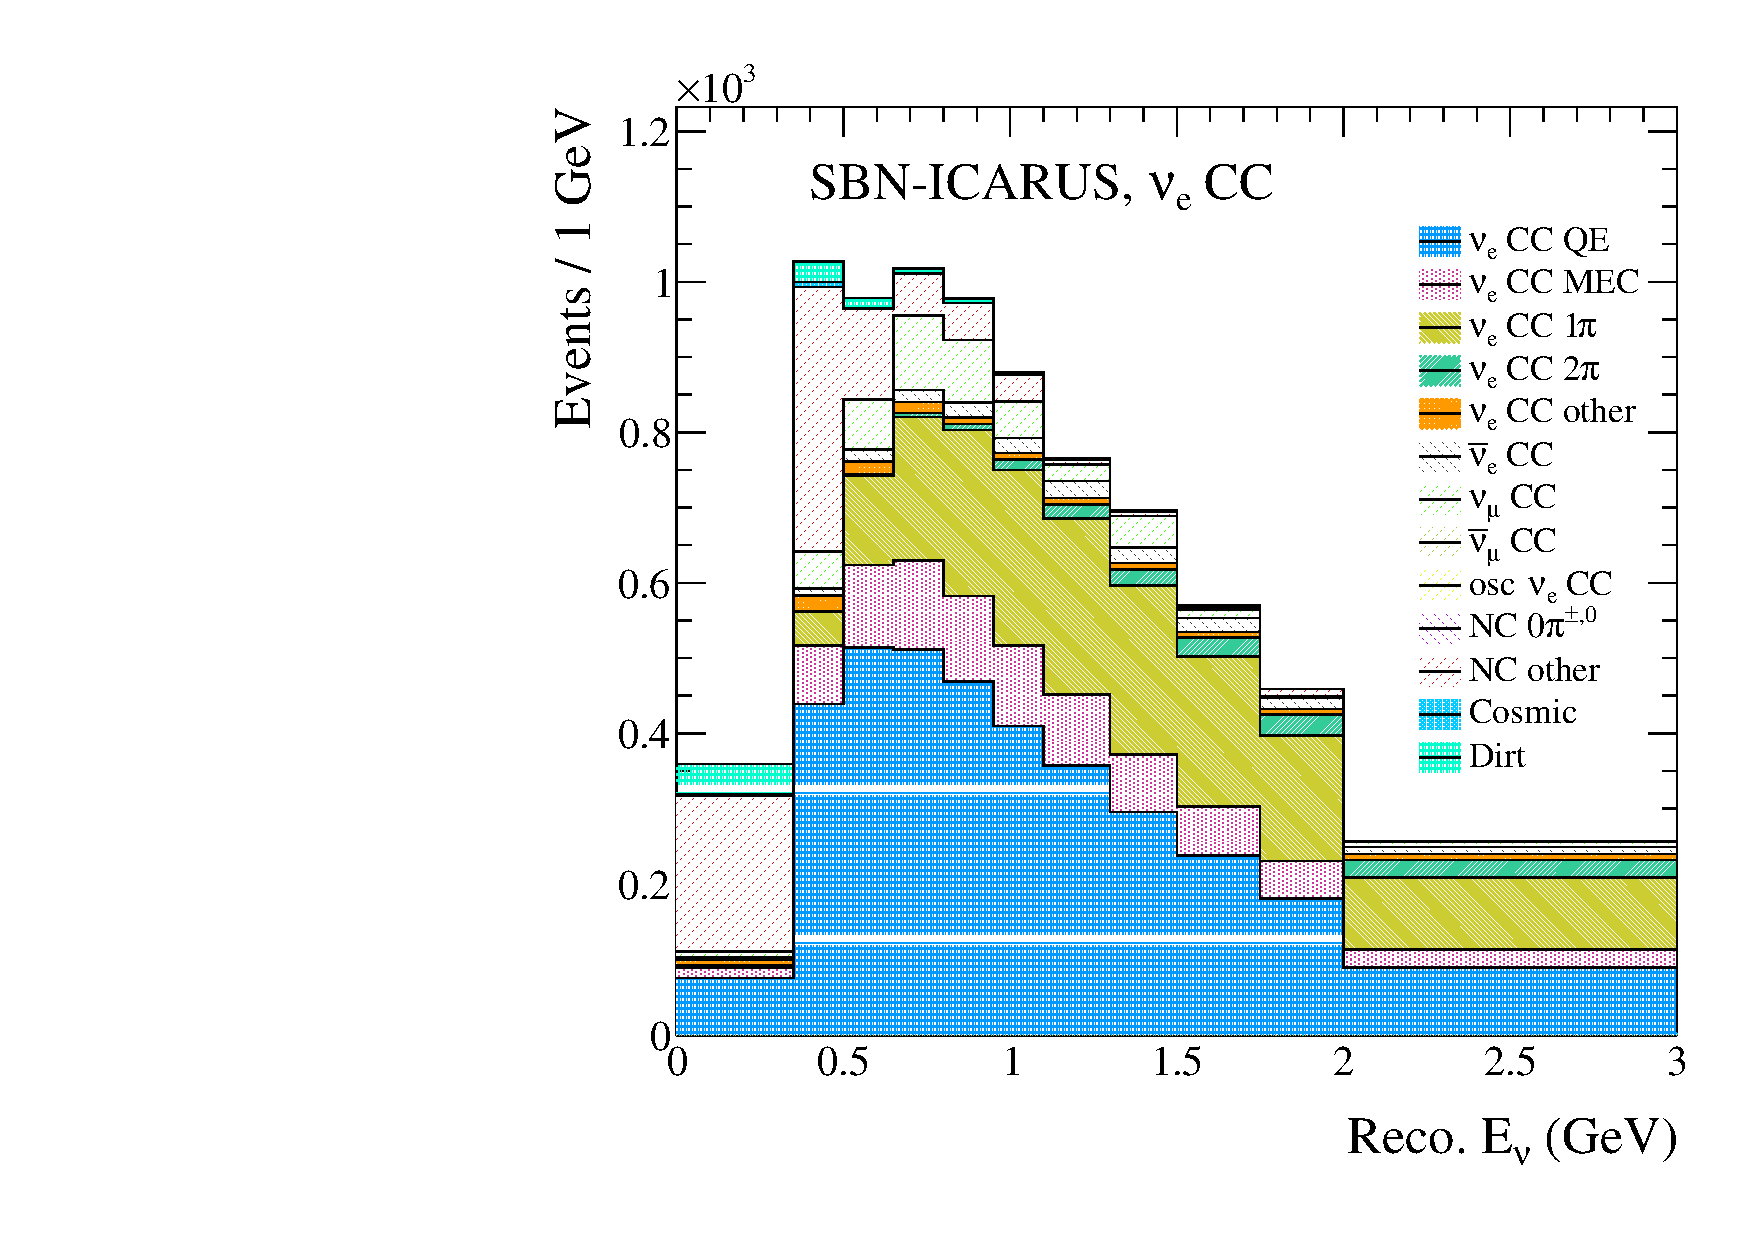
\includegraphics[width=0.49\textwidth]{figures-chap6/spectra/nue_nominal_spectrum_sbn_icarus_BNB_FHC_2_modes.pdf}}
  \captionsetup{width=0.49\textwidth}
  \parbox[b]{0.49\textwidth}%
  {
    \caption[SBN \nue CC inclusive reconstructed neutrino energy spectra.]{SBND (top-left), MicroBooNE (top-right) and ICARUS (bottom)
    reconstructed neutrino energy spectra constructed from the samples of $\nue$~CC~inclusive events. The spectra are broken down into the
    contributions from each neutrino interaction mode.\\ \phantom{.}\\}
    \label{fig:nominal_nue_spectra} 
  }
\end{figure}

\begin{figure}[h!]
  {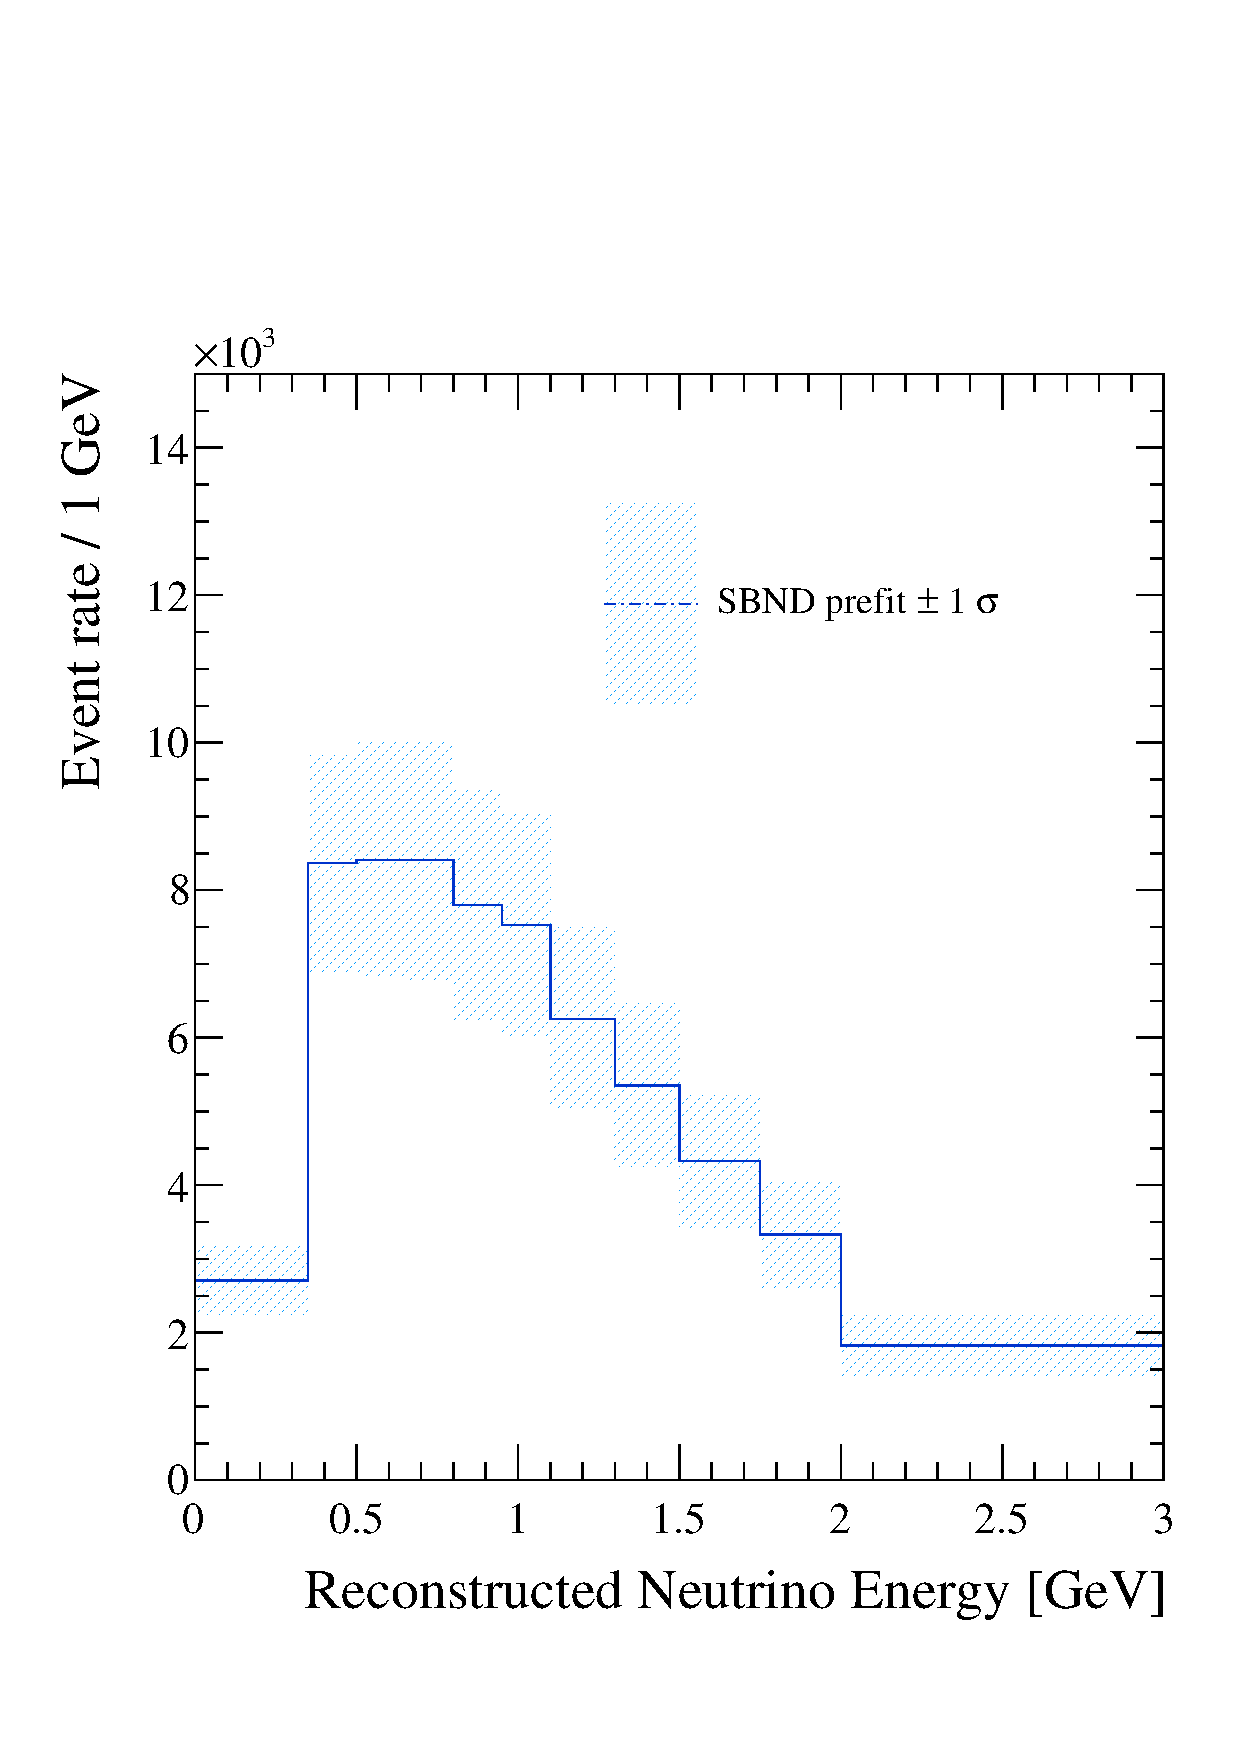
\includegraphics[width=0.49\textwidth]{figures-chap6/spectra/envelopes/sbnd_1sigma_prefit.pdf}}
  {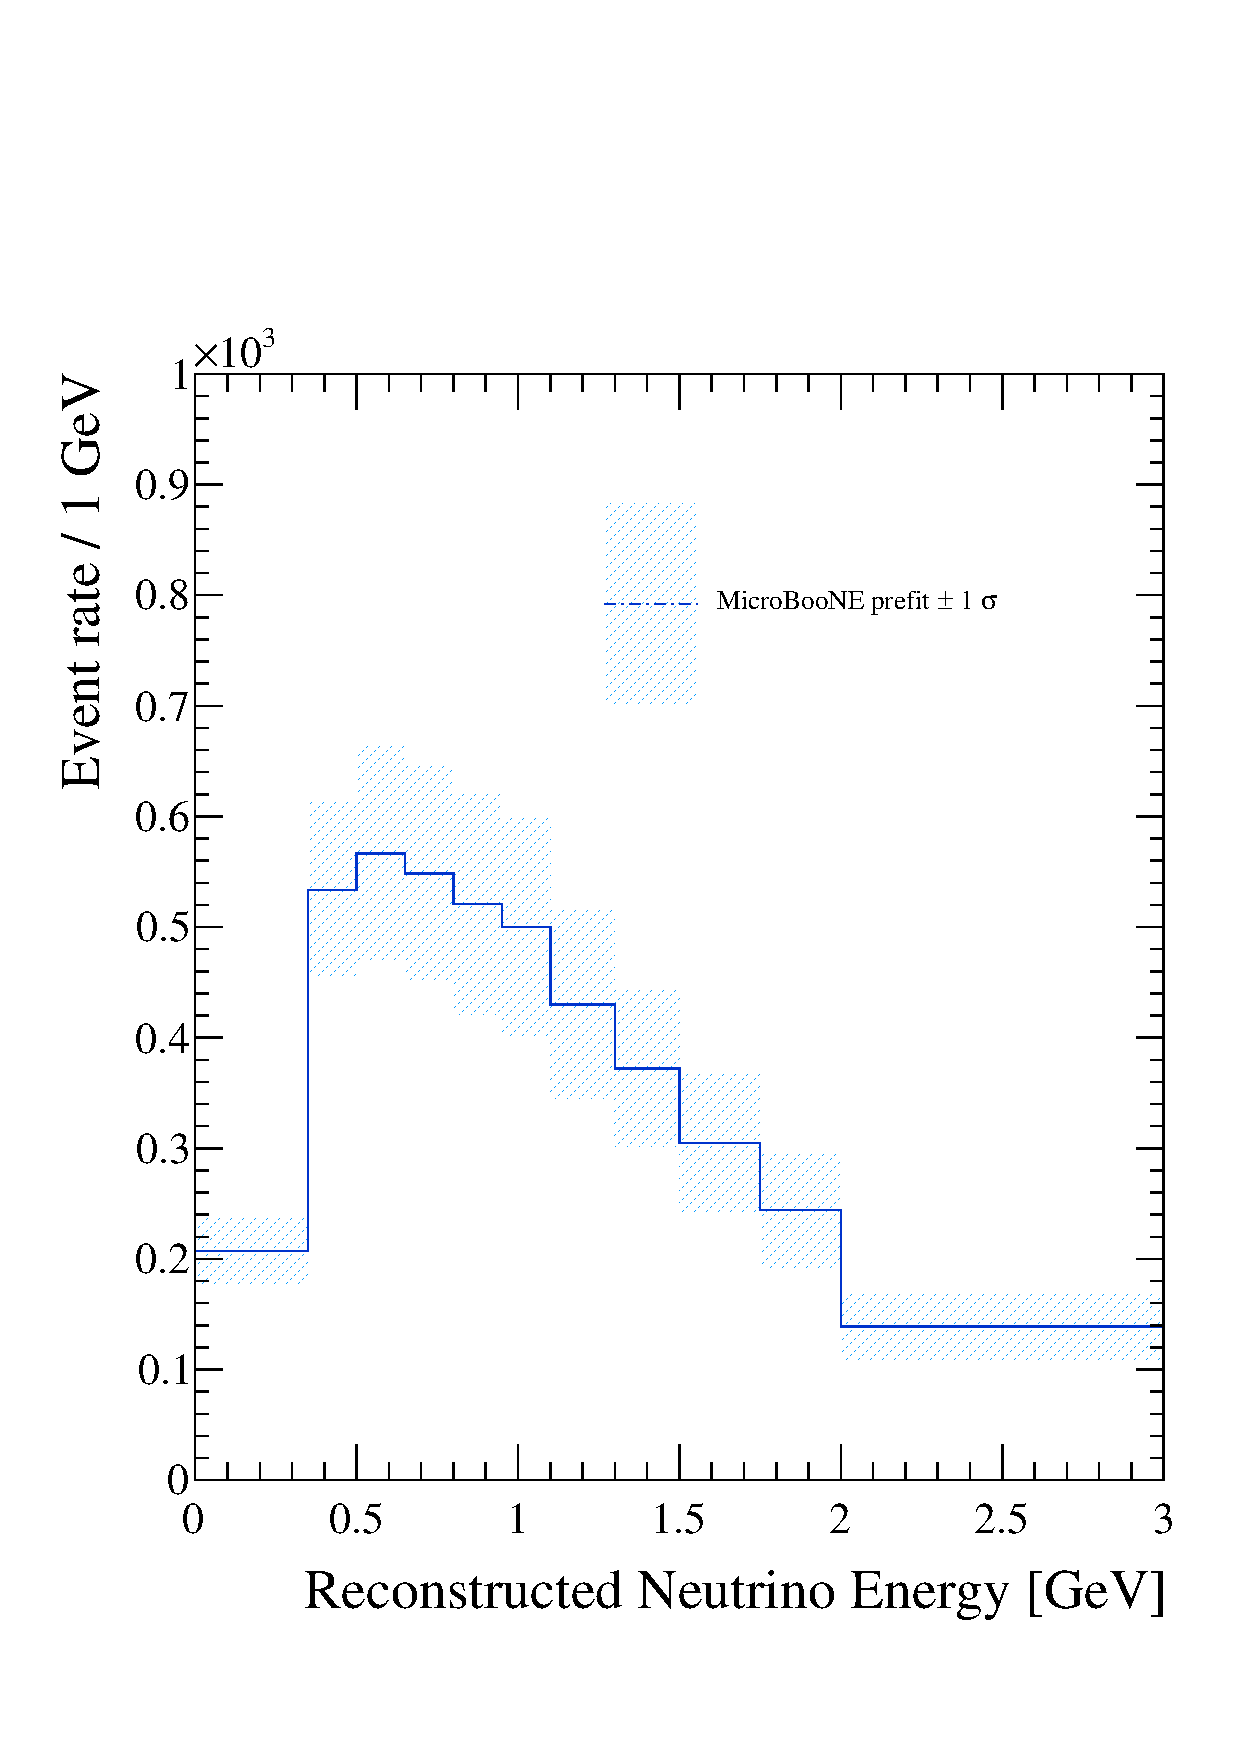
\includegraphics[width=0.49\textwidth]{figures-chap6/spectra/envelopes/uboone_1sigma_prefit.pdf}}
  {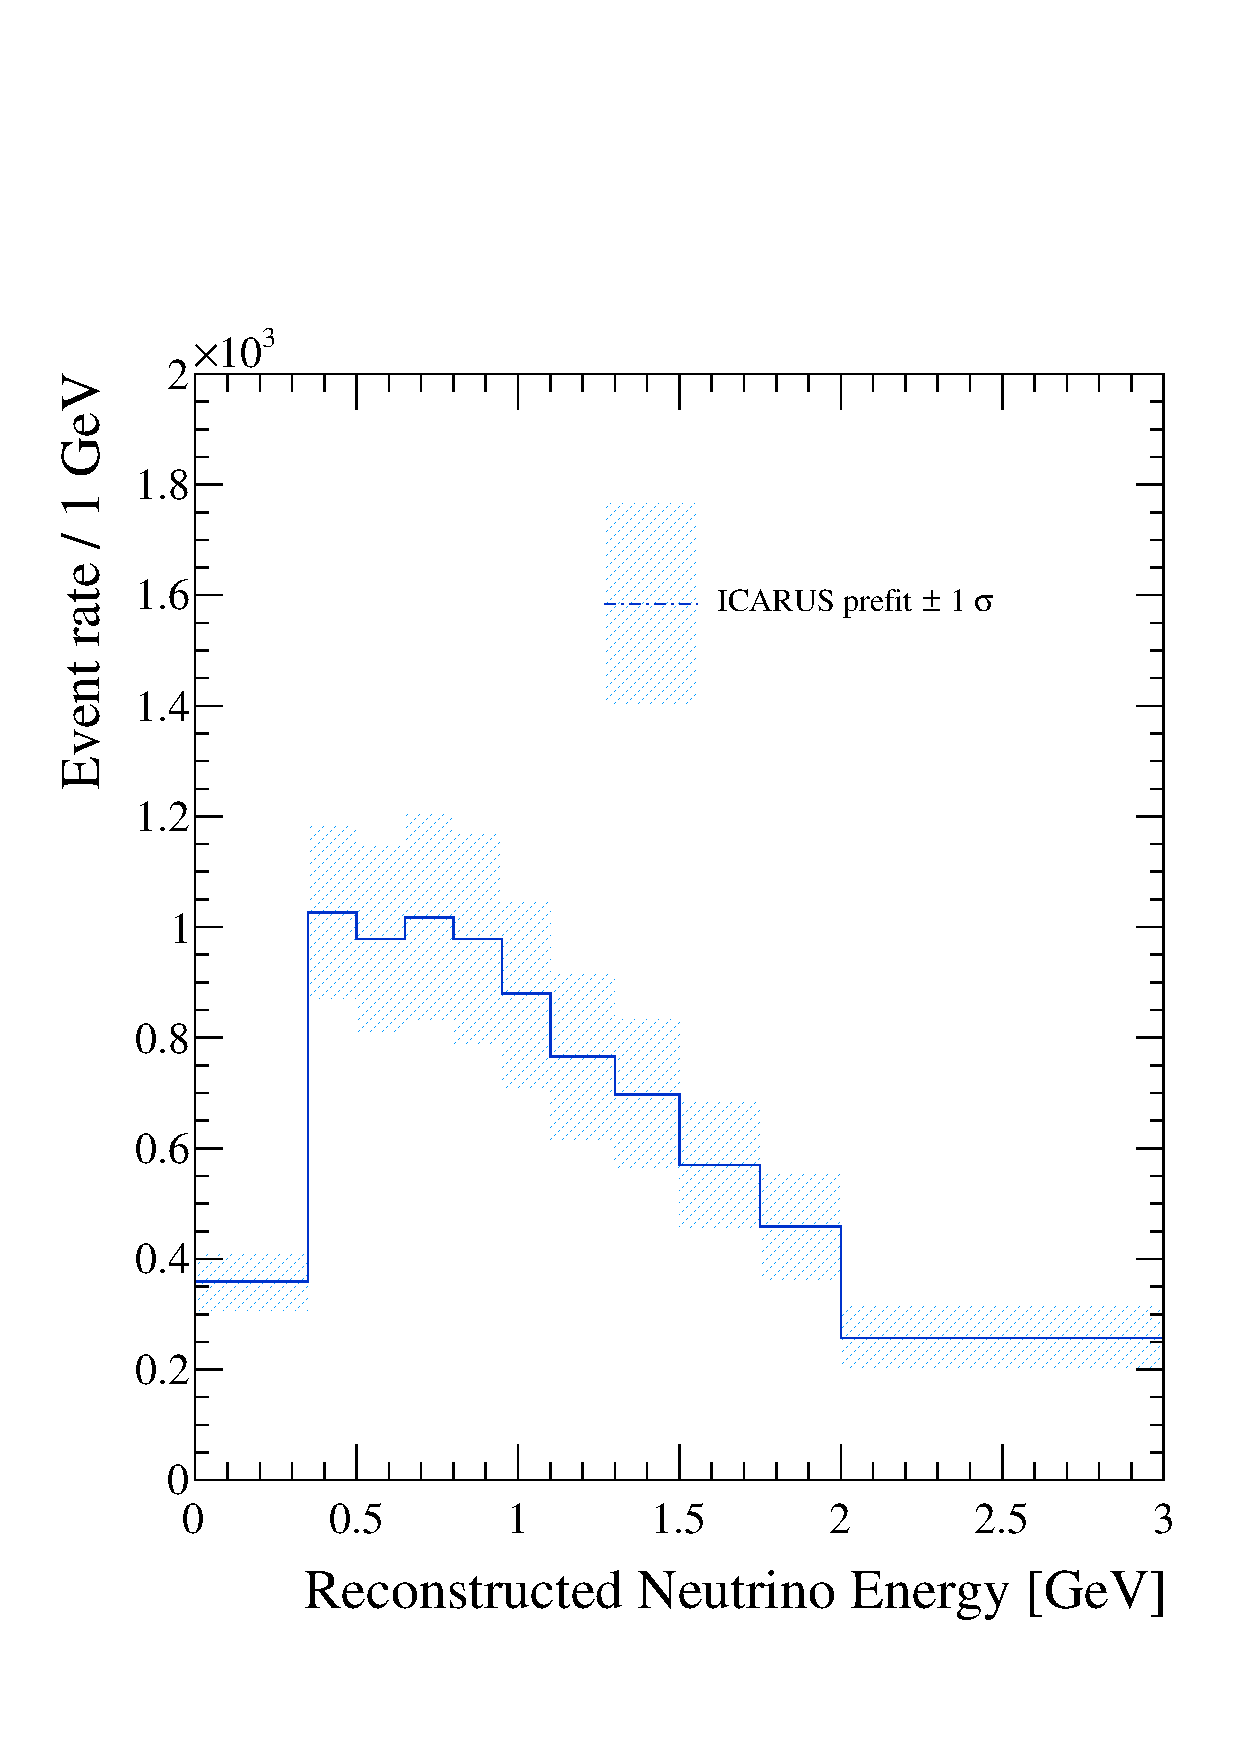
\includegraphics[width=0.49\textwidth]{figures-chap6/spectra/envelopes/icarus_1sigma_prefit.pdf}}
  \captionsetup{width=0.49\textwidth}
  \parbox[b]{0.49\textwidth}%
  {
    \caption[SBN \nue CC inclusive reconstructed neutrino energy spectra with a 1$\sigma$ prefit envelopes.]{SBND (top-left), MicroBooNE (top-right) and ICARUS (bottom) integrated reconstructed neutrino energy spectra constructed from the samples of $\nue$~CC~inclusive events. A 1$\sigma$ prefit uncertainty envelope from the flux and interaction systematics is also shown. \\\phantom{.}\\\phantom{.}\\\phantom{.}\\}
    \label{fig:nominal_nue_spectra_1sigma_enevelope} 
  }
\end{figure}

\begin{figure}[h!]
    \centering
    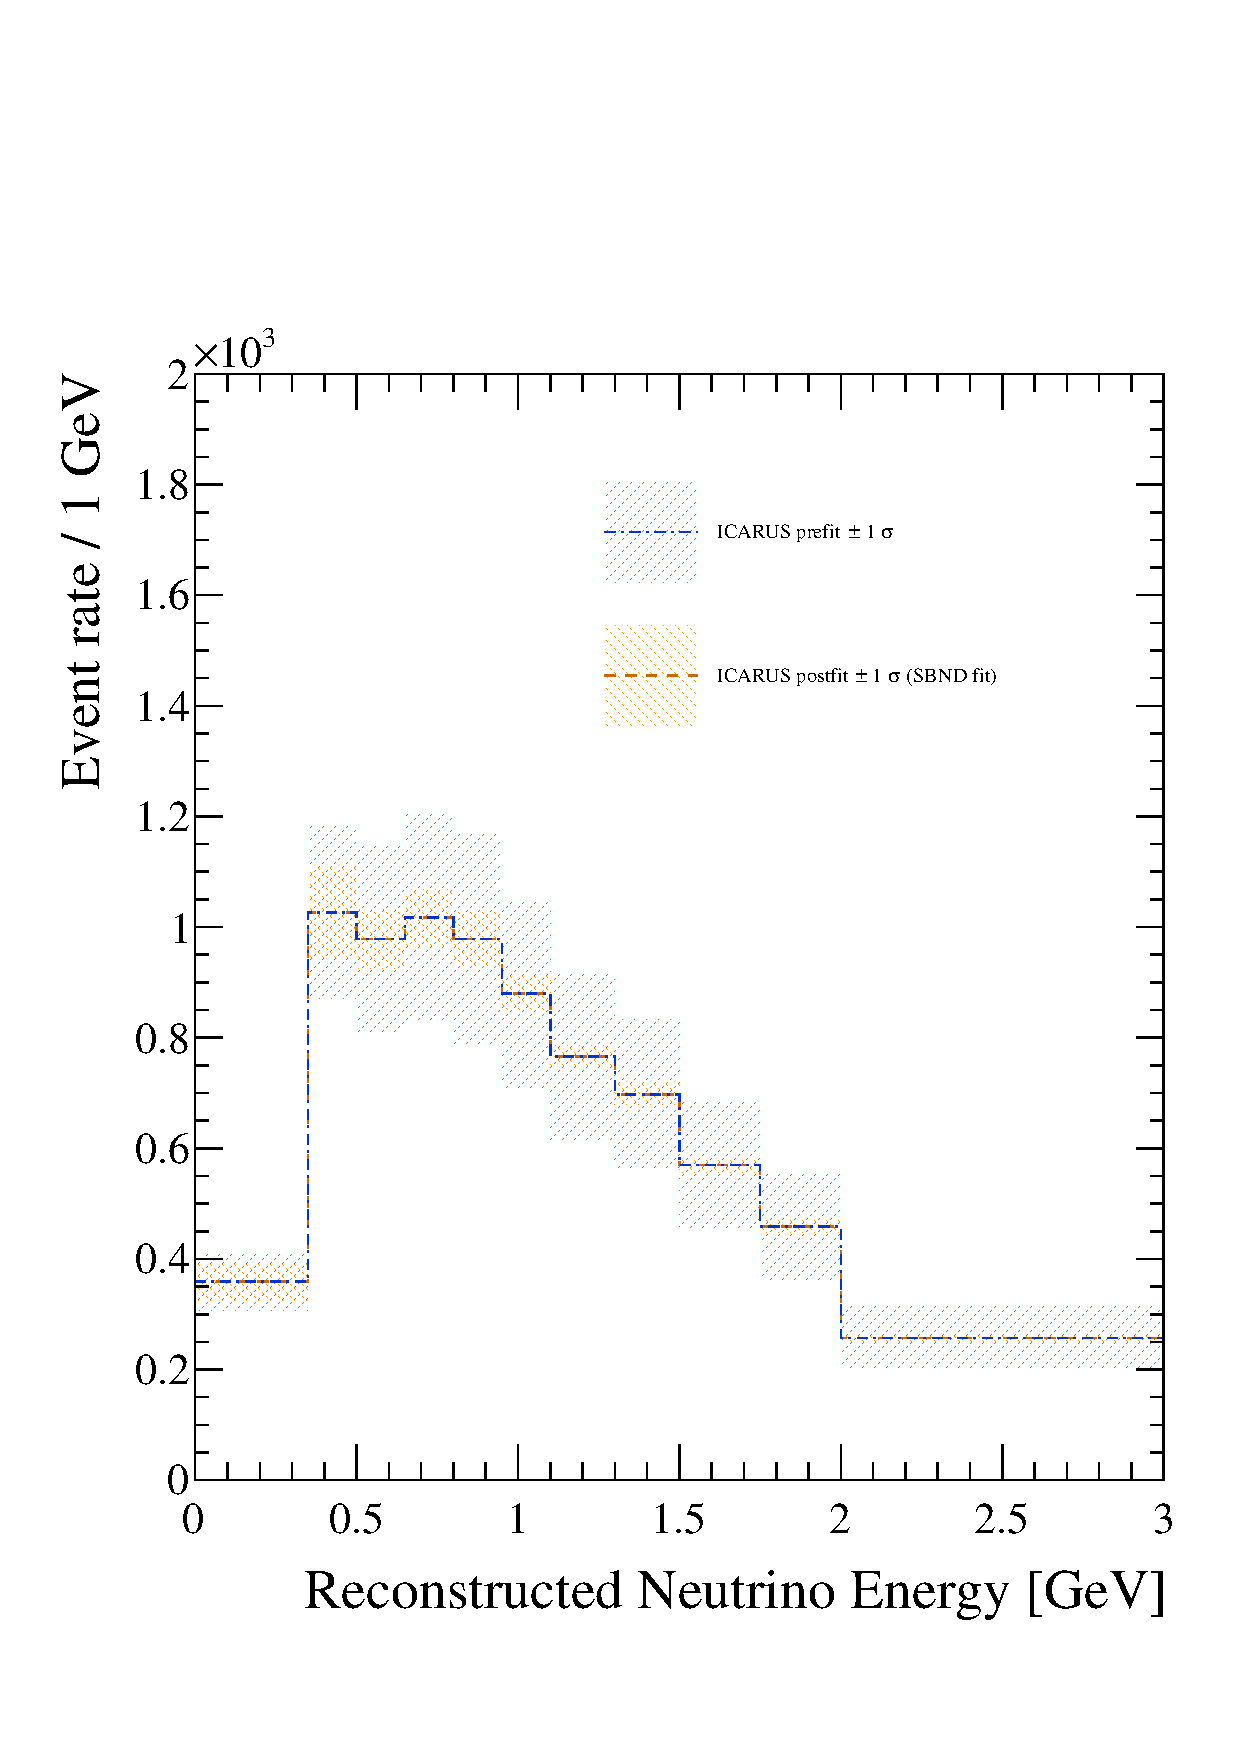
\includegraphics[width = \largefigwidth]{figures-chap6/spectra/envelopes/icarus_pre_post_fit_nue.pdf}
    \caption[ICARUS \nue CC inclusive neutrino energy spectra with a 1$\sigma$ prefit and postfit envelope.]{ICARUS integrated reconstructed neutrino energy spectrum constructed from the samples of \nue~CC~inclusive events. The $1\sigma$ prefit envelope is shown as well as a $1\sigma$ postfit envelope based on an \gls{sbnd} fit. The reduction in size of the error envelope when going from prefit to postfit shows the impact of \gls{sbnd} on improving the accuracy of the ICARUS prediction.}
    \label{fig:icarus_pre_post_fit}
\end{figure}

\clearpage
\subsection{Impact of Systematic Uncertainties}\label{sec:star_plot_study}

%\textcolor{red}{Not sure where best to put this section? Here or along with the sensitivity curves.}

To assess the impact of the different systematic parameters on the oscillation parameters the following study is performed;
\begin{enumerate}
    \item Generate a toy experiment with a given oscillation signal with a single systematic parameter, $f_i$, set to $\pm1\sigma$ from its nominal value and all other systematic parameters are set to their nominal value.
    \item Perform a fit on the toy experiment with $f_i$ fixed to its nominal value. Both the oscillation parameters and all the systematic parameters are initially set to their nominal value and are allowed to float with the exception of $f_i$. The other systematic parameters are allowed to float in order to obtain the best possible agreement between the fit and the toy experiment.
    \item Steps 1. and 2. are then repeated for all \textit{i} systematic parameters of interest. Both the +1$\sigma$ and -1$\sigma$ variations should be performed for each systematic parameter since the effect on the oscillation parameters is typically not symmetric.  
\end{enumerate}
If $f_i$ were allowed to float it would be expected that the fit would be able to recover the same oscillation parameters used in the toy experiment since the same \gls{mc} was used for the toy experiment and the fit. By fixing $f_i$ to its nominal value in the fit, the fit is forced to make a mistake. This results in the fit remapping the changes in $f_i$ to the oscillation parameters (and the other systematic parameters). 

This study was performed for the \nue appearance and disappearance channels using oscillation parameters $\sin^2{2\theta}_{\mu e} = 0.003$, 
$\Delta m^2_{41} = 1.32$ eV$^2$ and 
$\sin^2{2\theta}_{ee} = 0.4$, $\Delta m^2_{41} = 3$ eV$^2$ respectively and includes the results from all uncorrelated systematic parameters. The results are shown in \FigureRef{fig:nue_app_osc_param_pulls} and \FigureRef{fig:nue_disapp_osc_param_pulls}. For both oscillation parameters, the ratio of their value after performing the fit to their nominal value, $\mathcal{R}$, are shown after having varied $f_i$ by $\pm 1 \sigma$. The ratios shown in \FigureRef{fig:nue_app_osc_param_pulls} and \FigureRef{fig:nue_disapp_osc_param_pulls} are always $\geq 1$ by construction since $\mathcal{R}$ is defined as,
\begin{equation}
    \mathcal{R} = \begin{cases}
    \frac{\zeta_{fit}}{\zeta_{nom}}, & \text{if } \zeta_{fit} > \zeta_{nom} \\
    \frac{\zeta_{nom}}{\zeta_{fit}}, &\text{if } \zeta_{nom} > \zeta_{fit},
    \end{cases}
\end{equation}
where $\zeta \in \{\sin^2{2\theta}, \Delta m^2_{41}\}$ and the subscript \textit{nom} and \textit{fit} refer to the nominal value of the oscillation parameters and the values after performing the fit respectively. The arrows are colour coded such that black corresponds to the case where $\zeta_{fit} > \zeta_{nom}$ and red corresponds to the case where $\zeta_{nom} > \zeta_{fit}$.

\begin{figure}[h!]
    \centering
    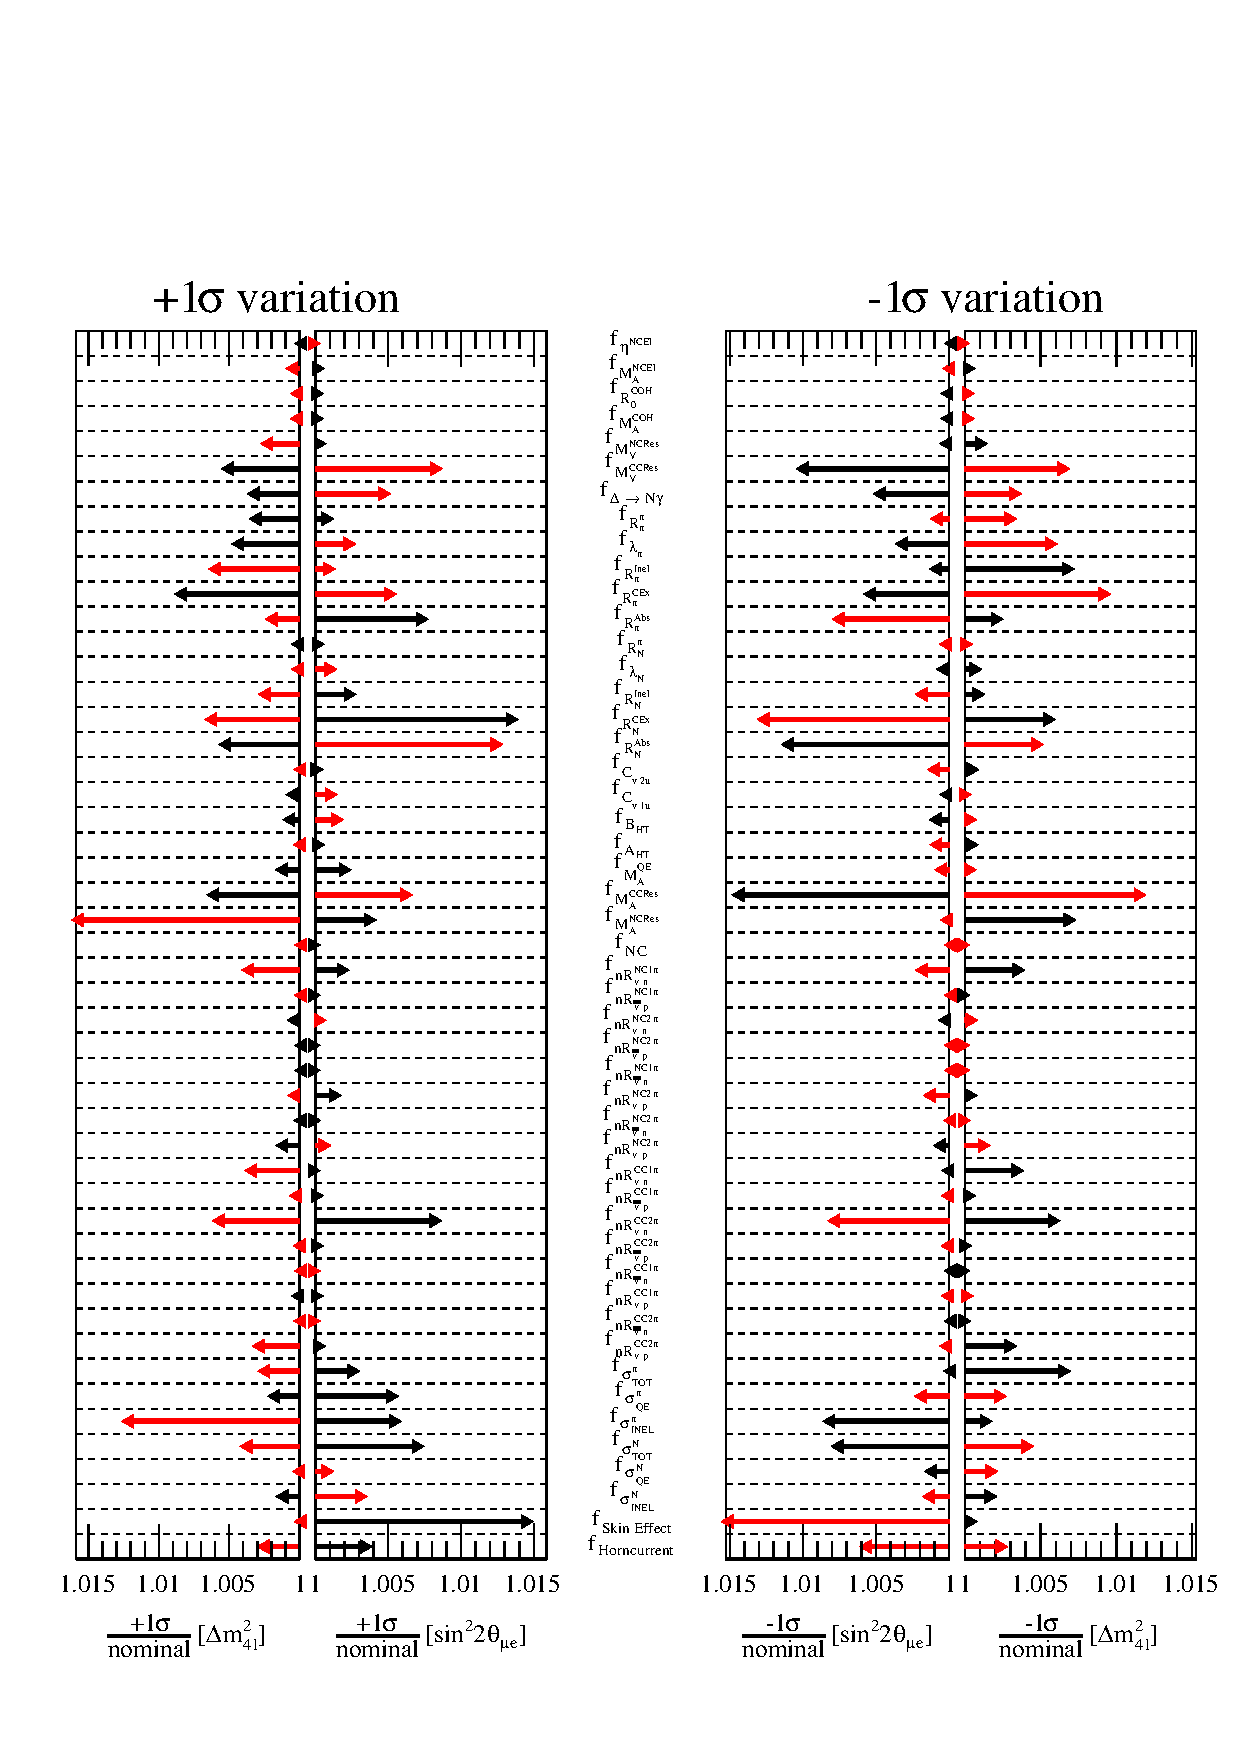
\includegraphics[width = \textwidth]{figures-chap6/star_plot/nue_app_pulls_2.pdf}
    \caption[\nue appearance oscillation parameter pulls due to varying a single systematic parameter by $\pm1\sigma$.]{The variation in the \nue appearance oscillation parameters due to varying a single systematic parameter at a time by $\pm1\sigma$.}
    \label{fig:nue_app_osc_param_pulls}
\end{figure}

\begin{figure}[h!]
    \centering
    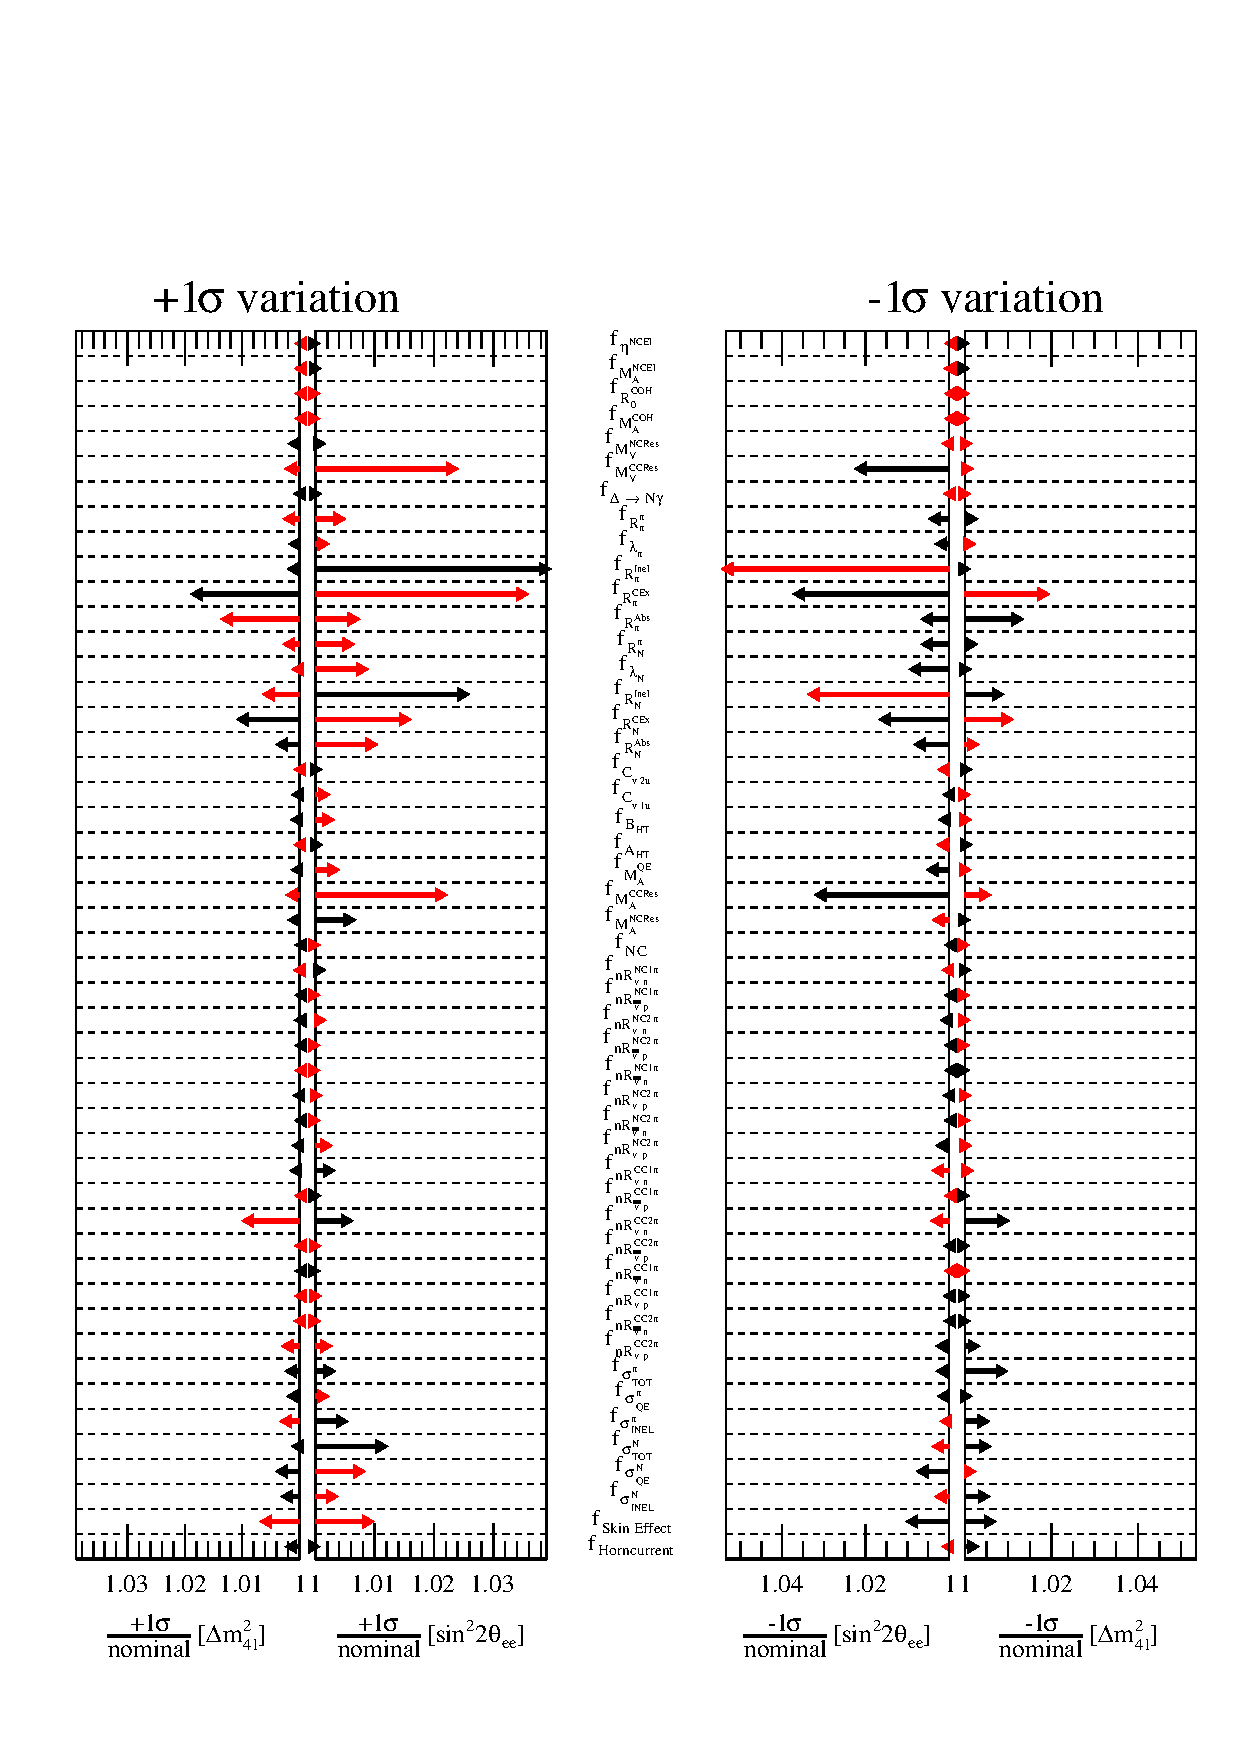
\includegraphics[width = \textwidth]{figures-chap6/star_plot/nue_dsisapp_pulls_2.pdf}
    \caption[\nue disappearance oscillation parameter pulls due to varying a single systematic parameter by $\pm1\sigma$.]{The variation in the \nue disappearance oscillation parameters due to varying a single systematic parameter at a time by $\pm1\sigma$.}
    \label{fig:nue_disapp_osc_param_pulls}
\end{figure}


\clearpage


\subsection{Expected Oscillation Signal}

Assuming that mixing with a light sterile neutrino occurs, a change to the nominal event rate will be observed. Since the oscillation channels are currently considered as stand-alone analyses, this will either result in an increase or decrease in the event rate depending on whether an appearance or disappearance channel is considered. 

\subsubsection{\texorpdfstring{\nue Appearance Analysis}{nue Appearance Analysis}}\label{sec:nue_app}

The \nue appearance channel is concerned with oscillations from \numu to \nue meaning an increase in the event rate is expected. This is shown in \FigureRef{fig:nue_spectra_with_osc_overlay} where the nominal event rate breakdown is shown as in \FigureRef{fig:nominal_nue_spectra} but overlayed with an integrated spectrum that was produced with oscillation parameters \mbox{$\sin^2{2\theta_{\mu e}} = 0.003$} and $\Delta m^2_{41} = 1.32 \text{ eV}^2$. The oscillation signal seen for these parameters in \gls{sbnd} is small whereas for \gls{microboone} and \gls{icarus} it is substantial which is consistent with what is seen in \FigureRef{fig:osc_probability}. This highlights the fact that \gls{sbnd} will largely be used to constrain systematic parameters due to observing no or very few oscillated events with the oscillation signal being largely left to \gls{microboone} and \gls{icarus}. 


\begin{figure}[h!]
  {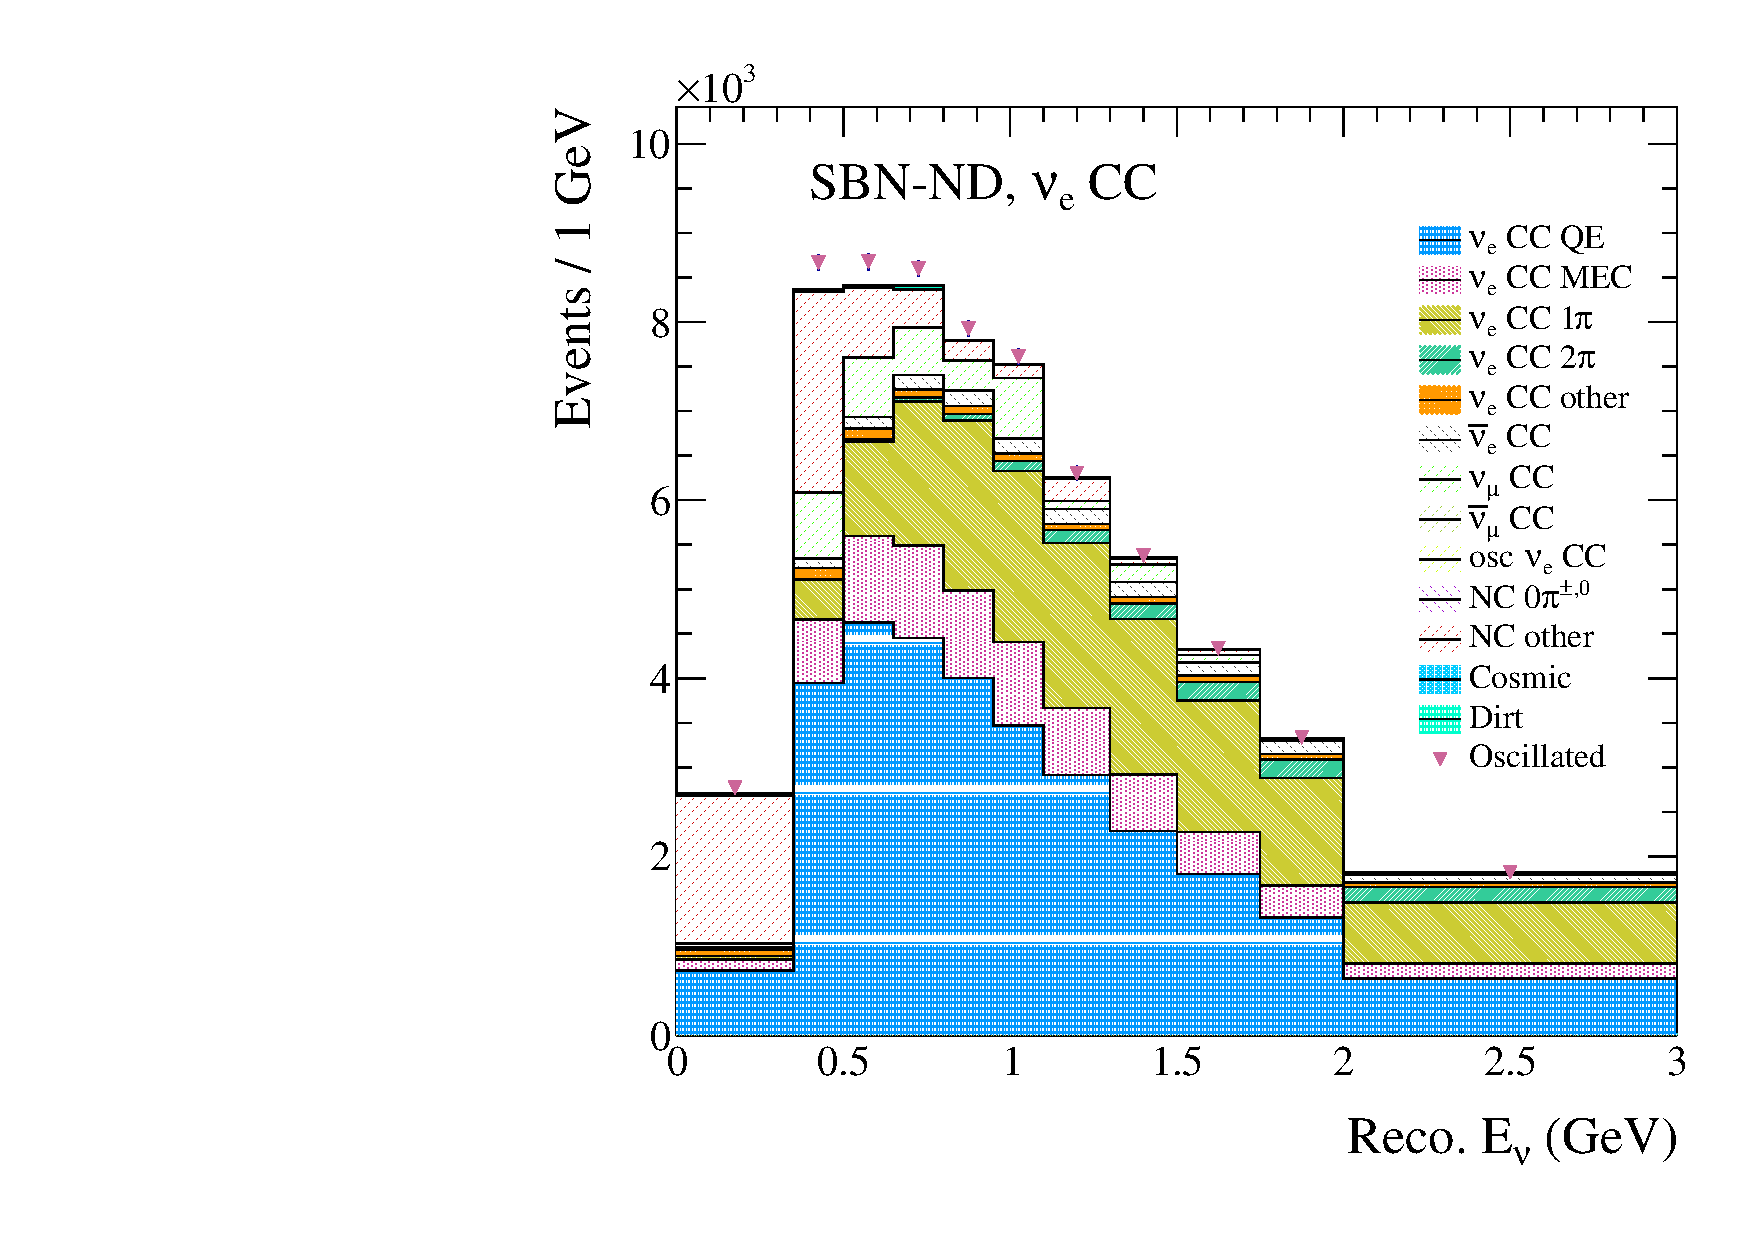
\includegraphics[width=0.49\textwidth]{figures-chap6/spectra/nue_app_dmsq_1.32_sinsq_0.003_overlay_spectrum_sbn_nd_BNB_FHC_0_modes.pdf}}
  {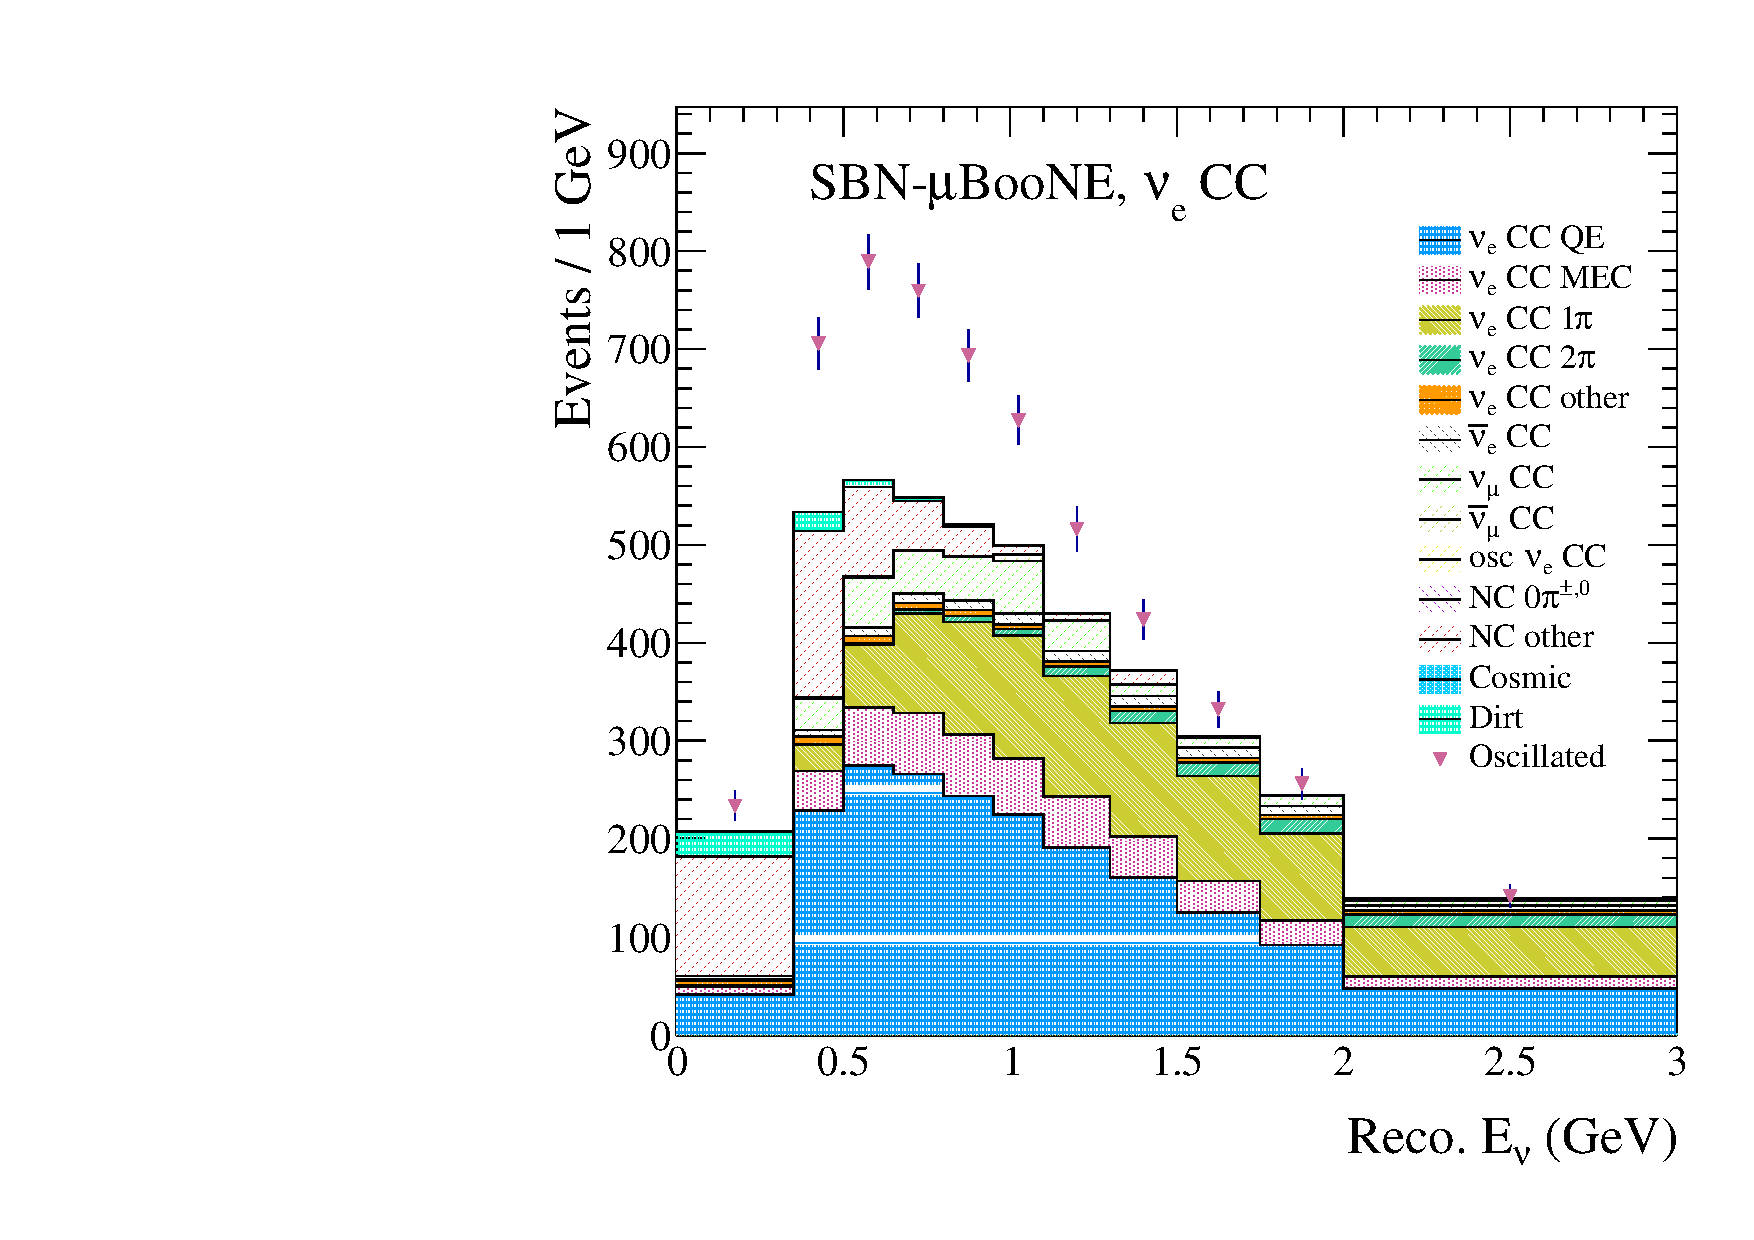
\includegraphics[width=0.49\textwidth]{figures-chap6/spectra/nue_app_dmsq_1.32_sinsq_0.003_overlay_spectrum_sbn_uboone_BNB_FHC_1_modes.pdf}}
  {\includegraphics[width=0.49\textwidth]{figures-chap6/spectra/nue_app_dmsq_1.32_sinsq_0.003_overlay_spectrum_sbn_icarus_BNB_FHC_2_modes.pdf}}
  \captionsetup{width=0.49\textwidth}
  \parbox[b]{0.49\textwidth}%
  {
    \caption[SBN \nue appearance CC inclusive reconstructed neutrino energy spectra with oscillated spectrum overlayed.]{The nominal spectra as in \FigureRef{fig:nominal_nue_spectra} but an additional integrated oscillated spectrum with oscillation parameters, $\sin^2{2\theta_{\mu e}} = 0.003$ and $\Delta m^2_{41} = 1.32$ eV$^2$ has been overlayed showing the increase in event rate. \\\phantom{.}\\\phantom{.}\\\phantom{.}\\
    \label{fig:nue_spectra_with_osc_overlay}}
    }
\end{figure}

\newpage
The top left plot of Figure~\ref{fig:Nue_app_spectra_ratios} shows the \nue appearance statistical only exclusion contour and allowed region from fits combining all three \gls{sbn} detectors. The details of constructing sensitivity contours within \gls{sbn} are detailed in \SectionRef{sec:sensitivites}. The injected point $\Delta m^2_{41} = 1.32$ eV$^2$, $\sin^2{2\theta_{\mu e}} = 0.003$, used when producing the allowed region is shown along with two further points on the exclusion contour at $\Delta m^2_{41} = 1$ eV$^2$, $\sin^2{2\theta_{\mu e}} = 0.0014$ and $\Delta m^2_{41} = 100$ eV$^2$, $\sin^2{2\theta_{\mu e}} = 0.0005$. \nue appearance spectra are produced using oscillation parameters corresponding to each of these three points for each of the three SBN detectors. The ratio of each of these oscillated spectra to the nominal for each detector are shown in the remaining plots in Figure~\ref{fig:Nue_app_spectra_ratios} and highlight the expected oscillation signal.


\begin{figure}[h!]
    \centering
    \includegraphics[width = 0.49\textwidth, height = 0.47\textwidth]{figures-chap6/overlays/nue_app_stat_osc_markers.pdf}
    \includegraphics[width = 0.49\textwidth]{figures-chap6/spectra/nue_app_spectra_ratio_sbnd.pdf}
    \includegraphics[width = 0.49\textwidth]{figures-chap6/spectra/nue_app_spectra_ratio_uboone.pdf}
    \includegraphics[width = 0.49\textwidth]{figures-chap6/spectra/nue_app_spectra_ratio_icarus.pdf}
    \caption[Ratio of \nue appearance spectra with the oscillation parameters shown on the statistical only contour.]{\nue appearance stat-only exclusion contour and allowed region. The injected point at $\sin^2{2\theta_{\mu e}} = 0.003$, $\Delta m^2_{41}$ = 1.32 eV$^2$ used for the allowed region is shown along with two further points at $\sin^2{2\theta_{\mu e}} = 0.0014$, $\Delta m^2_{41}$ = 1 eV$^2$ and   $\sin^2{2\theta_{\mu e}} = 0.0005$, $\Delta m^2_{41}$ = 100 eV$^2$ (top left). The ratio of spectra with oscillation parameters corresponding to the three points mentioned versus nominal are shown for \gls{sbnd} (top right), \gls{microboone} (bottom left) and \gls{icarus} (bottom right).}
    \label{fig:Nue_app_spectra_ratios}
\end{figure}


\subsubsection{\texorpdfstring{\nue Disappearance Analysis}{nue Disappearance Analysis}}

Mirroring the \nue appearance channel, the \nue disappearance channel observes a reduction in the nominal \nue event rate. This is shown in \FigureRef{fig:nue_disapp_spectra} where the integrated spectrum produced with oscillation parameters $\sin^2{2\theta_{ee}} = 0.4$ and $\Delta m^2_{41} = 3 \text{ eV}^2$ has been overlayed onto the breakdown of the nominal spectrum for each of the three detectors. As is the case for \nue appearance, the oscillation signal is relatively small in \gls{sbnd} whereas both \gls{microboone} and \gls{icarus} observe a much more significant signal. 

\begin{figure}[h!]
  {\includegraphics[width=0.49\textwidth]{figures-chap6/spectra/nue_disapp_dmsq_3_sinsq_0.4_overlay_spectrum_sbn_nd_BNB_FHC_0_modes.pdf}}
  {\includegraphics[width=0.49\textwidth]{figures-chap6/spectra/nue_disapp_dmsq_3_sinsq_0.4_overlay_spectrum_sbn_uboone_BNB_FHC_1_modes.pdf}}
  {\includegraphics[width=0.49\textwidth]{figures-chap6/spectra/nue_disapp_dmsq_3_sinsq_0.4_overlay_spectrum_sbn_icarus_BNB_FHC_2_modes.pdf}}
  \captionsetup{width=0.49\textwidth}
  \parbox[b]{0.49\textwidth}%
  {
    \caption[SBN \nue disappearance CC inclusive reconstructed neutrino energy spectra with oscillated spectrum overlayed]{The nominal spectra as in \FigureRef{fig:nominal_nue_spectra} but an additional integrated oscillated spectrum with oscillation parameters, $\sin^2{2\theta_{ee}} = 0.4$ and $\Delta m^2_{41} = 3$ eV$^2$ has been overlayed which shows the decrease in event rate.\\\phantom{.}\\\phantom{.}\\\phantom{.}\\}
    \label{fig:nue_disapp_spectra} 
  }
\end{figure}

The top left plot of Figure~\ref{fig:nue_disapp_spectra_ratios} shows the \nue disappearance statistical only exclusion contour and allowed region from fits combining all three \gls{sbn} detectors. The injected point \mbox{$\Delta m^2_{41} = 3$~eV$^2$}, $\sin^2{2\theta_{\mu e}} = 0.4$, used when producing the allowed region is shown along with two further points on the exclusion contour at \mbox{$\Delta m^2_{41} = 1$ eV$^2$}, $\sin^2{2\theta_{\mu e}} = 0.29$ and $\Delta m^2_{41} = 100$~eV$^2$, $\sin^2{2\theta_{\mu e}} = 0.085$. \nue disappearance spectra are produced using oscillation parameters corresponding to each of these three points for each of the three SBN detectors. The ratio of each of these oscillated spectra to the nominal for each detector are shown in the remaining plots in Figure~\ref{fig:nue_disapp_spectra_ratios} and highlight the expected oscillation signal.

\begin{figure}[h!]
    \centering
    \includegraphics[width = 0.49\textwidth]{figures-chap6/overlays/nue_disapp_stat_osc_markers.pdf}
    \includegraphics[width = 0.49\textwidth]{figures-chap6/spectra/nue_disapp_spectra_ratio_sbnd.pdf}
    \includegraphics[width = 0.49\textwidth]{figures-chap6/spectra/nue_disapp_spectra_ratio_uboone.pdf}
    \includegraphics[width = 0.49\textwidth]{figures-chap6/spectra/nue_disapp_spectra_ratio_icarus.pdf}
    \caption[Ratio of \nue disappearance spectra with the oscillation parameters shown on the statistical only contour.]{\nue disappearance stat-only exclusion contour and allowed region. The injected point at $\sin^2{2\theta_{ee}} = 0.4$, $\Delta m^2_{41}$ = 3 eV$^2$ used for the allowed region is shown along with two further points at $\sin^2{2\theta_{ee}} = 0.29$, $\Delta m^2_{41}$ = 1 eV$^2$ and \mbox{$\sin^2{2\theta_{ee}} = 0.085$}, \mbox{$\Delta m^2_{41}$ = 100 eV$^2$} (top left). The ratio of spectra with oscillation parameters corresponding to the three points mentioned versus nominal are shown for \gls{sbnd} (top right), \gls{microboone} (bottom left) and \gls{icarus} (bottom right).}
    \label{fig:nue_disapp_spectra_ratios}
\end{figure}



\clearpage


\section{SBN Sensitivity Contour Construction}\label{sec:sensitivites}

The relevant phase space for each of the three analysis channels considered is split into a $40 \times 40$ grid. This number was chosen in order to find a balance between having sufficient granularity when constructing contours without having excessive computing times. The dimensions of the phase space considered are different for each analysis channel and are listed in \TableRef{table:analysis_channel_phase_space}. Fits are performed for each of the $40 \times 40$ points where the oscillation parameters are fixed and the systematic parameters, if any, are allowed to float up to $\pm5\sigma$ from their nominal value. Once the fits have been produced, a contour of constant $\chi^2$ is constructed. The $\chi^2$ value is chosen such that it corresponds to a certain confidence level, \textit{CL}, which for \gls{sbn} analyses is typically 5$\sigma$. The critical value of $\chi^2$, $\chi^2_{critical}$, corresponding to a 5$\sigma$ confidence level along with a number of other $\chi^2_{critical}$ values with their associated confidence levels which are commonly seen in literature are outlined in \TableRef{table:critical_chi2_values}. An example of a 2D $\chi^2$ surface with exclusion contours at 90\%, 3$\sigma$ and 5$\sigma$ confidence levels for the \nue appearance channel is shown in \FigureRef{fig:nue_app_chisq_surface}. The contours have been produced for the entire \gls{sbn} program with the inclusion of flux and interaction systematics.

\begin{table}[h!]
\begin{tabular}{lcc}
\multicolumn{1}{c}{\multirow{2}{*}{Analysis Channel}} & \multicolumn{2}{c}{Phase Space Considered} \\
\multicolumn{1}{c}{} & $\sin^2{2\theta}$ & $\Delta m_{41}^2$ \\ \hline
\numu Disappearance & $\theta_{\mu\mu}$: [10$^{-3}$ -- 1] & [10$^{-2}$ -- 10$^2$] eV$^2$ \\
\nue Appearance & $\theta_{\mu e}$: [10$^{-5}$ -- 1] & [10$^{-2}$ -- 10$^2$] eV$^2$ \\
\nue Disappearance & $\theta_{ee}$: [10$^{-2}$ -- 1] & [10$^{-2}$ -- 10$^2$] eV$^2$
\end{tabular}
\caption[The phase space considered for each of the SBN analyses.]{The phase space considered when constructing contours for each of the three oscillation channels within \gls{sbn}.}
\label{table:analysis_channel_phase_space}
\end{table}

\begin{table}[h!]
\begin{tabular}{lllllll}
 Confidence level & 68\% & 90\% & 95\% & 99\% & 3$\sigma$ & 5$\sigma$ \\ \hline
$\chi^2_{critical}$ & 0.23 & 1.64 & 2.71 & 5.41 & 7.74 & 23.66
\end{tabular}
\caption[$\chi^2_{critical}$ values for various confidence levels.]{The $\chi^2_{critical}$ values corresponding to various confidence levels which are commonly used when performing sensitivity studies. The confidence levels and $\chi^2_{critical}$ are related via $CL = \int_0^{\chi^2_{critical}} \frac{e^{-x/2}x^{u/2-1}}{2^{u/2}\Gamma(u/2)} dx$, where \textit{u} is the degrees of freedom (in this case 1) and $\Gamma$ is the Gamma function \cite{critical_chi2_book}.}
\label{table:critical_chi2_values}
\end{table}

\begin{figure}[h!]
    \centering
    \includegraphics[width = \largefigwidth]{figures-chap6/exclusion_contours/nue_app_03d1_chi2_surface.pdf}
    \caption[\nue appearance contours overlayed on the $\chi^2$ surface.]{The \nue appearance $\chi^2$ surface from fits including flux and interaction systematics. Contours of constant $\chi^2$ values which correspond to 90\%, 3$\sigma$ and 5$\sigma$ confidence levels have been overlayed onto the surface.}
    \label{fig:nue_app_chisq_surface}
\end{figure}


The complete \nue appearance exclusion sensitivities and allowed regions for both the statistical-only case and with the inclusion of flux and interaction systematics are shown in \FigureRef{fig:nue_app_global_sensitivity} for the entire \gls{sbn} program alongside external limits from the \gls{lsnd} and \gls{karmen} experiments \cite{LSND_KARMEN_nue_app_contour}. For comparison purposes, it should be noted that the contours produced for the \gls{sbn} program are at the $5\sigma$ confidence level whereas the results from both \gls{lsnd} and \gls{karmen} are at the 99\% confidence level. The results from \gls{sbn} shows an improvement over the \gls{karmen} results for essentially all $\Delta m^2_{41}$ values and the allowed region is largely consistent with the \gls{lsnd} result. 


\begin{figure}[h!]
    \centering
    \includegraphics[width = \largefigwidth]{figures-chap6/overlays/valor_overlays_nue_app.pdf}
    \caption[\nue appearance contours with external limits.]{\nue appearance exclusion contours and allowed regions for the stat only case and with flux and interaction systematic uncertainties included. External limits from the \gls{lsnd} and \gls{karmen} experiments have been overlayed \cite{LSND_KARMEN_nue_app_contour}. (The confidence intervals for each contour are shown in the legend and it should be noted that those from external limits are not the same as those from the contours produced for the \gls{sbn} program.)}
    \label{fig:nue_app_global_sensitivity}
\end{figure}

The complete \nue disappearance exclusion sensitivities and allowed regions for both the statistical-only case and with the inclusion of flux and interaction systematics are shown in \FigureRef{fig:nue_disapp_global_sensitivity} for the entire \gls{sbn} program alongside external limits from the ND280 detector which serves as one of the near detectors as part of the \gls{t2k} experiment \cite{t2k_experiment}. The results for the \gls{sbn} program are shown at a 5$\sigma$ confidence level whereas the allowed region from the \gls{t2k} experiment is shown at both 68\% and 90\% confidence level and the exclusion contour is at a 95\% confidence level \cite{T2K_nue_disapp_contour}. The results from \gls{sbn} exclude a substantial portion of the \gls{t2k} allowed region with the exclusion limits at high $\Delta m^2_{41}$ not being as strong for the current comparison. 

\begin{figure}
    \centering
    \includegraphics[width = \largefigwidth]{figures-chap6/overlays/valor_overlays_nue_disapp.pdf}
    \caption[\nue disappearance contours with external limits.]{\nue disappearance exclusion contours and allowed regions for the stat only case and with flux and interaction systematic uncertainties included. External limits from the \gls{t2k} experiments have been overlayed \cite{T2K_nue_disapp_contour}. (The confidence intervals for each contour are shown in the legend and it should be noted that those from external limits are not the same as those from the contours produced for the \gls{sbn} program.)}
    \label{fig:nue_disapp_global_sensitivity}
\end{figure}


\clearpage
\section{Further Study on Sensitivities}

The sensitivity contours shown in \FigureRef{fig:nue_app_global_sensitivity} and \FigureRef{fig:nue_disapp_global_sensitivity} are produced from combined fits from all the three \gls{sbn} detectors with the inclusion of all the flux and interaction systematic uncertainties outlined in \SectionRef{sec:syst_uncertainties}.

Fits may, however, also be produced for an individual detector or any combination of multiple detectors. Additionally, there is complete freedom to choose which systematic parameters are included in the fits. This allows for the option to only include a single systematic parameter or an entire sub-group of parameters. 

This section will discuss the impact on the sensitivity contours due to;
\begin{itemize}
    \item Different combinations of individual and multiple detectors.
    \item The inclusion of a select number of individual systematic parameters. 
    \item The inclusion of each set of flux and systematic parameters.
    \item The inclusion of additional efficiency uncertainties.
    \item Tweaking the energy smearing used in the event selection based on results from \ChapterRef{chap:Energy_Reco}.
\end{itemize}

\subsection{Impact of Detector Combinations}

To see the impact that each detector has on the sensitivity contour, the left plot of \FigureRef{fig:nue_sensitivity_detector_contribution} shows the \nue appearance statistical-only sensitivity contours from each individual detector as well as all possible combinations (the black curve labelled ``SBN'' refers to a contour from combining all three detectors). It can be seen that for large $\Delta m^2_{41}$ (greater than $\sim$5 eV$^2$), that the \gls{sbnd} detector dominates the sensitivity whereas for small $\Delta m^2_{41}$ (less than $\sim$0.7 eV$^2$) the \gls{icarus} detector dominates. It should also be noted that only by combining the fits from all three detectors can the best sensitivities be obtained. Having this multi-detector design is one of the key advantages of the \gls{sbn} program. The right plot of \FigureRef{fig:nue_sensitivity_detector_contribution} is akin to the left one, but with the inclusion of flux and interaction systematics in the fits. Again, the improvements to the sensitivity are highlighted by combining multiple detectors. 

\begin{figure}[h!]
    \centering
    \includegraphics[width = 0.49\textwidth]{figures-chap6/exclusion_contours/nue_app_detector_combinations_stat_only.pdf}
    \includegraphics[width = 0.49\textwidth]{figures-chap6/exclusion_contours/nue_app_detector_combinations_stat+syst.pdf}
    \caption[\nue appearance sensitivities from different detector combinations.]{Contributions to the SBN \nue appearance sterile oscillation sensitivity from each detector and combinations of detectors in the SBN program. The statistical-only plots in the left-hand figure show that SBND is most sensitive to the region $\Delta m_{41}^{2} >$ $\sim$3 eV$^{2}$and ICARUS is most sensitive to $\Delta m_{41}^{2} <$ $\sim$3 eV$^{2}$. The right-hand figure includes flux and interaction systematic parameters and highlights the considerable improvement in the oscillation sensitivity when including multiple detectors in the fits.}
    \label{fig:nue_sensitivity_detector_contribution}
\end{figure}

Similar to \FigureRef{fig:nue_sensitivity_detector_contribution}, \FigureRef{fig:nue_disapp_sensitivity_detector_contribution} shows the \nue disappearance sensitivity from individual detectors and combinations of multiple detectors for both the statistical-only case (Left) and the case with flux and interaction systematics (Right). Again, \gls{sbnd} dominates the sensitivity at high mass splitting whereas \gls{icarus} is dominant for low mass splitting with the emphasis being on the improvement to the overall sensitivity when fits from all three \gls{sbn} detectors are combined.

\begin{figure}[h!]
    \centering
    \includegraphics[width = 0.49\textwidth]{figures-chap6/exclusion_contours/nue_disapp_detector_combinations_stat-only.pdf}
    \includegraphics[width = 0.49\textwidth]{figures-chap6/exclusion_contours/nue_disapp_detector_combinations_stat+syst.pdf}
    \caption[\nue disappearance sensitivities from different detector combinations.]{Contributions to the SBN \nue disappearance sterile oscillation sensitivity from each detector and combinations of detectors in the SBN program produced. The statistical-only plots in the left-hand figure show that SBND is most sensitive to the region $\Delta m_{41}^{2} > 3$~eV$^{2}$ and ICARUS is most sensitive below $\Delta m_{41}^{2} < 3$~eV$^{2}$. The right-hand figure includes flux and interaction systematic parameters and highlights the considerable improvement in the oscillation sensitivity when including multiple detectors in the fits.}
    \label{fig:nue_disapp_sensitivity_detector_contribution}
\end{figure}

\newpage

\subsection{Impact of Systematic Parameters}

The impact of the $f_{M_V^{CCRes}}$, $f_{M_A^{CCRes}}$, $f_{R_N^{C Ex}}$ and $f_{\sigma^{\pi}_{INEL}}$ parameters on the \nue appearance exclusion sensitivities are shown in \FigureRef{fig:nue_app_single_param}. The parameters were applied one at a time and chosen as some that showed the largest variations in \FigureRef{fig:nue_app_osc_param_pulls}, ensuring at least one parameter is from each systematic subgroup. Similarly, the $f_{M_V^{CCRes}}$, $f_{M_A^{CCRes}}$, $f_{R_{\pi}^{C Ex}}$ and $f_{expskin}$ parameters were used for the \nue disappearance channel and the results are shown in \FigureRef{fig::nue_disapp_single_param}. Both the statistical-only contour and the one including all the flux and interaction systematics are shown for comparison. It should be noted that single parameters may contribute significantly to the total reduction in sensitivity from the inclusion of all systematic parameters. Additionally, the systematics considered were chosen based on a study which used an injected signal meaning the large impact seen there may not be directly mapped to an exclusion contour which gives a possible reason for the relatively minor impact seen due to $f_{\sigma^{\pi}_{INEL}}$ and $f_{R_{\pi}^{C Ex}}$.

\begin{figure}[h!]
    \centering
    \includegraphics[width = 0.49\textwidth]{figures-chap6/exclusion_contours/single_param/nue_app_single_param.pdf}
    \includegraphics[width =0.49\textwidth]{figures-chap6/exclusion_contours/single_param/nue_app_single_param_ratio.pdf}
    \caption[\nue appearance exclusion contours with the inclusion of a single systematic parameter at a time.]{Left: \nue appearance exclusion contours with the inclusion of a single systematic parameter at a time. The systematic parameters considered are $f_{M_V^{CCRes}}$, $f_{M_A^{CCRes}}$, $f_{R_N^{C Ex}}$ and $f_{\sigma^{\pi}_{INEL}}$. Right: The ratio of the exclusion contours with the inclusion of a single systematic parameter to the statistical-only contour.}
    \label{fig:nue_app_single_param}
\end{figure}

\begin{figure}[h!]
    \centering
    \includegraphics[width = 0.49\textwidth]{figures-chap6/exclusion_contours/single_param/nue_disapp_single_param.pdf}
    \includegraphics[width =0.49\textwidth]{figures-chap6/exclusion_contours/single_param/nue_disapp_single_param_ratio.pdf}
    \caption[\nue disappearance exclusion contours with the inclusion of a single systematic parameter at a time.]{Left: \nue disappearance exclusion contours with the inclusion of a single systematic parameter at a time. The systematic parameters considered are $f_{M_V^{CCRes}}$, $f_{M_A^{CCRes}}$, $f_{R_{\pi}^{C Ex}}$ and $f_{expskin}$. Right: The ratio of the exclusion contours with the inclusion of a single systematic parameter to the statistical-only contour.}
    \label{fig::nue_disapp_single_param}
\end{figure}

\newpage

The results from applying the flux, proposal interaction, modern interaction and proposal + modern interaction systematic subgroups for the \nue appearance channel is shown in the left plot of  \FigureRef{fig:nue_app_syst_group_sensitivities}. This highlights the reduction in sensitivity when individually applying each systematic subgroup when compared to the statistical-only case. The right-hand plot of \FigureRef{fig:nue_app_syst_group_sensitivities} shows the ratio of the exclusion contours to the statistical-only case. This gives a clearer measure of the impact on the sensitivity in $\sin^2{2\theta_{\mu e}}$ space. It follows that the interaction systematics have the biggest impact on the sensitivity which in turn are dominated by the modern set of interaction parameters. The proposal set of interaction parameters have the smallest impact with the magnitude of the impact from the flux parameters being somewhere in between the two sets of interaction parameters. 

\begin{figure}[h!]
    \centering
    \includegraphics[width = 0.49\textwidth]{figures-chap6/exclusion_contours/nue_app_syst_groups.pdf}
    \includegraphics[width = 0.49\textwidth]{figures-chap6/exclusion_contours/nue_app_syst_groups_ratios.pdf}
    \caption[Impact of the different systematic parameter groups on the \nue appearance sensitivity.]{The left plot shows the reduction in sensitivity from the stat-only contour when including each set of systematic parameters in the fits. The right plot shows the relative location of each systematic contour in $\sin^{2}2\theta_{\mu e}$ space, with respect to the statistical-only case for the active region of $\Delta m_{41}^{2}$ phase space.}
    \label{fig:nue_app_syst_group_sensitivities}
\end{figure}

The relative contribution of the different systematic groups to the overall exclusion contour for \nue disappearance is shown in \FigureRef{fig:nue_disapp_syst_groups} and is comparable to the \nue appearance case. The interaction systematics again have the largest impact, the majority of which is due to the modern set of parameters. The proposal set of parameters have the smallest impact with the magnitude of the impact from the flux parameters being somewhere in between the two sets of interaction parameters.

\begin{figure}[h!]
    \centering
    \includegraphics[width = 0.49\textwidth]{figures-chap6/exclusion_contours/nue_disapp_syst_groups.pdf}
    \includegraphics[width = 0.49\textwidth]{figures-chap6/exclusion_contours/nue_disapp_syst_groups_ratios.pdf}
    \caption[\nue app sensitivity reduction from different systematic groups.]{The left plot shows the reduction in sensitivity from the stat-only contour when including each set of systematic parameters in the fits. The right plot shows the relative location of each systematic contour in $\sin^{2}2\theta_{ee}$ space, with respect to the statistical-only case for the active region of $\Delta m_{41}^{2}$ phase space.}
    \label{fig:nue_disapp_syst_groups}
\end{figure}

\newpage

To further assess the reduction in sensitivities due to specific parameters or parameter groups, allowed regions have been constructed using the same injected signal as was used for the study done in \SectionRef{sec:star_plot_study}. 
\FigureRef{fig:nue_injected_single_param} shows the change in allowed regions from applying the same set of single systematic parameters for both the \nue appearance and disappearance channels as was done for the exclusion contours. Both the statistical-only contour and the one including flux and interaction systematics have again been included for comparison.  Additionally, the allowed region with the inclusion of a single parameter are shown along with the corresponding contour from the entire associated set of systematic parameters for the \nue appearance and \nue disappearance channels in \FigureRef{fig:nue_app_single_syst_sets} and \FigureRef{fig:nue_disapp_single_syst_sets} respectively. Unlike for the exclusion contours, the  $f_{\sigma^{\pi}_{INEL}}$ and $f_{R_{\pi}^{C Ex}}$ parameters don't show the smallest change across the entire parameter space. The change is comparable to the other parameters for at least some of the parameter space which is more consistent with the size of the impact seen in \SectionRef{sec:star_plot_study}.

\begin{figure}[h!]
    \centering
    \includegraphics[width = 0.49\textwidth]{figures-chap6/allowed_regions/single_param/nue_app.pdf}
    \includegraphics[width =0.49\textwidth]{figures-chap6/allowed_regions/single_param/nue_disapp.pdf}
    \caption[\nue appearance and disappearance allowed regions with the inclusion of a single systematic parameter at a time.]{\nue appearance and disappearance allowed regions with the inclusion of a single systematic parameter at a time. The injected signal for \nue appearance is $\sin^2{2\theta_{\mu e}} = 0.003$, $\Delta m^2_{41}$ = 1.32 eV$^2$ whereas the injected signal for \nue disappearance is $\sin^2{2\theta_{ee}} = 0.4$, $\Delta m^2_{41}$ = 3 eV$^2$. The systematic parameters considered for the \nue appearance channel are $f_{M_V^{CCRes}}$, $f_{M_A^{CCRes}}$, $f_{R_N^{C Ex}}$ and $f_{\sigma^{\pi}_{INEL}}$ (Left) and the systematic parameters considered for the \nue disappearance channel are $f_{M_V^{CCRes}}$, $f_{M_A^{CCRes}}$, $f_{R_{\pi}^{C Ex}}$ and $f_{expskin}$ (Right).}
    \label{fig:nue_injected_single_param}
\end{figure}

\begin{figure}[h!]
  {\includegraphics[width=0.49\textwidth]{figures-chap6/allowed_regions/single_param/nue_app_flux.pdf}}
  {\includegraphics[width=0.49\textwidth]{figures-chap6/allowed_regions/single_param/nue_app_proposal.pdf}}
  {\includegraphics[width=0.49\textwidth]{figures-chap6/allowed_regions/single_param/nue_app_modern.pdf}}
  \captionsetup{width=0.49\textwidth}
  \parbox[b]{0.49\textwidth}%
  {
    \caption[The \nue appearance allowed regions with the inclusion of single systematic parameters compared to the region with the inclusion of all parameters in the associated set.]{The \nue appearance allowed region from an injected signal at $\sin^2{2\theta_{\mu e}} = 0.003$, $\Delta m^2_{41}$ = 1.32 eV$^2$ showing the impact of the $f_{\sigma^{\pi}_{INEL}}$ compared to the total flux systematics (Top Left), the impact of $f_{M_A^{CCRes}}$ compared to the total proposal systematics (Top Right) and the impact of both $f_{M_V^{CCRes}}$ and $f_{R_{\pi}^{C Ex}}$ on the total modern systematics (Bottom Left). The stat only and total flux + interaction contours have been included for comparison. \\}
    \label{fig:nue_app_single_syst_sets} 
  }
\end{figure}

\begin{figure}[h!]
  {\includegraphics[width=0.49\textwidth]{figures-chap6/allowed_regions/single_param/nue_disapp_flux.pdf}}
  {\includegraphics[width=0.49\textwidth]{figures-chap6/allowed_regions/single_param/nue_disapp_proposal.pdf}}
  {\includegraphics[width=0.49\textwidth]{figures-chap6/allowed_regions/single_param/nue_disapp_modern.pdf}}
  \captionsetup{width=0.49\textwidth}
  \parbox[b]{0.49\textwidth}%
  {
  \caption[The \nue disappearance allowed regions with the inclusion of single systematic parameters compared to the region with the inclusion of all parameters in the associated set.]{The \nue disappearance allowed region from an injected signal at $\sin^2{2\theta_{ee}} = 0.4$, $\Delta m^2_{41}$ = 3 eV$^2$ showing the impact of the $f_{expskin}$ compared to the total flux systematics (Top Left), the impact of $f_{M_A^{CCRes}}$ compared to the total proposal systematics (Top Right) and the impact of both $f_{M_V^{CCRes}}$ and $f_{R_N^{C Ex}}$ on the total modern systematics (Bottom Left). The stat only and total flux + interaction contours have been included for comparison. \\}
    \label{fig:nue_disapp_single_syst_sets} 
  }
\end{figure}
\clearpage

\subsection{Impact of Additional Efficiency Systematics}\label{Impact of Additional Efficiency Systematics}

As was mentioned in \SectionRef{sec:efficiency_syst}, efficiency systematics are not currently included in the \textit{standard} analyses. In order to get a measure of the possible impact of efficiency systematics on the sensitivity, various covariance matrices were produced following the scheme outlined in \SectionRef{sec:efficiency_syst}. Matrices were produced to investigate the impact of:
\begin{enumerate}
    \item Fully correlated errors only.
    \item Various combinations of uncorrelated errors with a fixed correlated error.
    \item Uncorrelated errors only applied to a single detector at a time.
    \item A poorly constrained uncorrelated error on a single set of bins.
\end{enumerate}
Unless otherwise stated, the uncertainties from efficiency covariance matrices are applied in addition to the flux and interaction systematics. 

The study on the impact of different efficiency uncertainties was first done for the \numu disappearance channel because it was expected that there would be a greater impact than for either of the \nue channels. This is because the typical event rate for the \numu channel is several orders of magnitude greater than that of \nue meaning that the \numu channel is systematics limited whereas the \nue channels may tend towards being statistics limited. Once a contour becomes statistics limited, continuing to apply additional systematic uncertainties will begin to have diminishing impacts. 

Sensitivities including efficiency uncertainties for the \numu disappearance channel are shown alongside the other figures in \AppendixRef{app:numu_disapp}. The impact of the efficiency uncertainties on both \nue channels is discussed below.


\subsubsection*{\texorpdfstring{Impact of Efficiency Systematics on \nue Appearance Sensitivities}{Impact of Efficiency Systematics on nue Appearance Sensitivities}}

In order to gauge the contribution of some typical efficiency uncertainty, \FigureRef{fig:nue_app_syst_groups+efficiency} shows the impact on the \nue appearance sensitivity from individual sets of systematic parameters as in \FigureRef{fig:nue_app_syst_group_sensitivities} but with the additional case where only a 2\% correlated + 2\% uncorrelated efficiency uncertainty has been applied. The impact of the efficiency uncertainty is comparable to the proposal interaction systematics having the smallest contribution to the sensitivity. 

\begin{figure}[h!]
    \centering
    \includegraphics[width = \largefigwidth]{figures-chap6/exclusion_contours/nue_app_syst_groups+det.pdf}
    \caption[\nue app sensitivity reduction from different systematic groups with a (2+2)\% efficiency uncertainty.]{The reduction in the \nue appearance sensitivity from the stat-only contour when including each set of systematic parameters in the fits. Similar to \FigureRef{fig:nue_app_syst_group_sensitivities} but with the addition of a 2\% correlated and 2\% uncorrelated efficiency uncertainty.}
    \label{fig:nue_app_syst_groups+efficiency}
\end{figure}

The reduction in sensitivity from applying a 10\% correlated uncertainty and a 2\% correlated + 2\% uncorrelated uncertainty on top of the standard flux and interaction systematics are shown in \FigureRef{fig:nue_app_corr_uncorr_error}. Since a correlated error of 10\% has a close to negligible impact, the results from applying correlated uncertainties less than 10\% as was done for the \numu channel have been omitted. Similarly, applying smaller uncorrelated uncertainties would again only have a minor impact so these have also been omitted.  

\begin{figure}[h!]
    \centering
    \includegraphics[width = \largefigwidth]{figures-chap6/exclusion_contours/efficiency_systematics/nue_app_cor_uncor.pdf}
    \caption[Impact of correlated and uncorrelated efficiency systematics on the \nue appearance sensitivity.]{The impact on the \nue appearance exclusion sensitivity by applying a 10\% fully correlated efficiency uncertainty to all bins and by applying 2\% fully correlated + 2\% uncorrelated efficiency uncertainty.}
    \label{fig:nue_app_corr_uncorr_error}
\end{figure}

\FigureRef{fig:nue_app_uncorrelated_per_detector} assess the impact of a 2\% uncorrelated uncertainty which is applied to each detector one at a time. Applying the uncertainty to \gls{microboone} and \gls{icarus} appears to have a negligible impact across all $\Delta m^2_{41}$ values. \gls{sbnd} has a relatively small impact at high $\Delta m^2_{41}$ values which resembles the loss in sensitivity that was seen by applying a 2\% correlated + 2\% uncorrelated uncertainty across all bins in \FigureRef{fig:nue_app_corr_uncorr_error}. It follows that any reduction in sensitivity due to efficiency uncertainties is driven by \gls{sbnd}. Since \gls{sbnd} is most sensitive to large $\Delta m^2_{41}$ values and has higher statistics than \gls{microboone} and \gls{icarus}, the results are consistent with the idea that \nue channel is close to becoming statistics limited. 

\begin{figure}[h!]
    \centering
    \includegraphics[width = \largefigwidth]{figures-chap6/exclusion_contours/efficiency_systematics/nue_app_2pct_uncor_per_detector.pdf}
    \caption[\nue app with a 2\% uncorrelated efficiency systematic for one detector only.]{The impact on the \nue appearance exclusion sensitivity by applying a 2\% uncorrelated efficiency uncertainty to a single one of the three \gls{sbn} detectors.}
    \label{fig:nue_app_uncorrelated_per_detector}
\end{figure}

%The impact of having a set of bins with a poorly constrained uncertainty was also studied using the same scheme that was outlined for the \numu case. Similar results were observed and are shown in \FigureRef{fig:nue_app_bulk_uncertainty}, albeit the change in sensitivity is much less prominent than for the \numu case. The background and low energy bins have the smallest impact with almost no visible difference whereas the peak and high energy bins do show some small reduction in the sensitivity. 

Instead of exploring the impact from fully correlated uncertainties or a constant uncorrelated uncertainty across all bins in a detector, \FigureRef{fig:nue_app_bulk_uncertainty} considers the case where a single set of bins are poorly constrained. The sets of bins considered are,
\begin{itemize}
    \item CC signal below the peak energy ($< 0.6$ GeV),
    \item CC signal at the peak energy ([0.6 - 1.0] GeV),
    \item CC signal above the peak energy ($> 1.0$ GeV),
    \item Background.
\end{itemize}
In each case, the uncorrelated uncertainty for the bins of interest are set to 2\% in each of the \gls{sbn} detectors, whilst the rest of the uncorrelated uncertainties are set to 0.5\% and the fully correlated uncertainty is fixed at 2\%. The background and low energy bins have the smallest impact with almost no visible difference whereas the peak and high energy bins do show some small reduction in the sensitivity at $\Delta m^2_{41}$ greater than 1 eV$^2$.

\begin{figure}[h!]
    \centering
    \includegraphics[width = \largefigwidth]{figures-chap6/exclusion_contours/efficiency_systematics/nue_app_2pct_cor_05pct_bulk_2pct_X_uncor.pdf}
    \caption[\nue appearance with poorly constrained efficiency systematic for a set of bins.]{The impact on the \nue appearance exclusion sensitivity by applying a 2\% fully correlated efficiency uncertainty for each of the \gls{sbn} detectors and a 0.5\% uncorrelated uncertainty for all but a single set of bins where the uncorrelated uncertainty is set to 2\%. The 'peak' energy bins are defined as those covering an energy range of [0.6,~1.0] GeV. The 'high' and 'low' energy bins are defined as those covering energies above and below the peak energy respectively and the 'bkg' bins are all the bins associated with background events. The set of bins of interest are applied to each of the three detectors.}
    \label{fig:nue_app_bulk_uncertainty}
\end{figure}



\clearpage

\subsubsection*{\texorpdfstring{Impact of Efficiency Systematics on \nue Disappearance Sensitivities}{Impact of Efficiency Systematics on nue Disappearance Sensitivities}}

As was done for \nue appearance, \FigureRef{fig:nue_disapp_syst_groups_detector} shows the impact from \nue disappearance sensitivity from individual sets of systematic parameters as in \FigureRef{fig:nue_disapp_syst_groups} but with the addition of a 2\% correlated + 2\% uncorrelated efficiency uncertainty. The efficiency uncertainty shows the smallest reduction in sensitivity across all ranges of $\Delta m_{41}^2 \gtrsim 3$ and is comparable to the other systematic sets at $\Delta m_{41}^2$ values below $\sim 3$.

\begin{figure}[h!]
    \centering
    \includegraphics[width = \largefigwidth]{figures-chap6/exclusion_contours/nue_disapp_syst_groups+det.pdf}
     \caption[\nue disappearance sensitivity reduction from different systematic groups with a (2+2)\% efficiency uncertainty.]{The reduction in the \nue disappearance sensitivity from the stat-only contour when including each set of systematic parameters in the fits. Similar to \FigureRef{fig:nue_disapp_syst_groups} but with the addition of a 2\% correlated and 2\% uncorrelated efficiency uncertainty.}
    \label{fig:nue_disapp_syst_groups_detector}
\end{figure}

Mirroring what was done for \nue appearance, \FigureRef{fig:nue_disapp_corr_uncorr} shows the impact of applying a 10\% correlated error and a 2\% correlated + 2\% uncorrelated error. The correlated error again has an almost negligible impact and whilst the uncorrelated error has a larger impact it is still relatively small. 

\begin{figure}[h!]
    \centering
    \includegraphics[width = \largefigwidth]{figures-chap6/exclusion_contours/efficiency_systematics/nue_disapp_cor_uncor.pdf}
    \caption[Impact of correlated and uncorrelated efficiency systematics on the \nue disappearance sensitivity.]{The impact on the \nue disappearance exclusion sensitivity by applying a 10\% fully correlated efficiency uncertainty to all bins and by applying 2\% fully correlated + 2\% uncorrelated efficiency uncertainty.}
    \label{fig:nue_disapp_corr_uncorr}
\end{figure}

A 2\% uncorrelated uncertainty is then applied to each detector one at a time. \FigureRef{fig:nue_disapp_uncorrelated_per_detector} shows that majority of the reduction is due to \gls{sbnd} at above $\Delta m_{41}^2 \sim 10$ (where \gls{sbnd} is dominant). Both \gls{microboone} and \gls{icarus} only have a minimal impact for any $\Delta m^2_{41}$ values. This is consistent with what is shown in \FigureRef{fig:nue_disapp_corr_uncorr}. 

\begin{figure}[h!]
    \centering
    \includegraphics[width = \largefigwidth]{figures-chap6/exclusion_contours/efficiency_systematics/nue_disapp_2pct_uncor_per_detector.pdf}
    \caption[\nue disapp with a 2\% uncorrelated efficiency systematic for one detector only.]{The impact on the \nue disappearance exclusion sensitivity by applying a 2\% uncorrelated efficiency uncertainty to a single one of the three \gls{sbn} detectors.}
    \label{fig:nue_disapp_uncorrelated_per_detector}
\end{figure}

\newpage
Finally, the impact of having a set of poorly constrained bins is investigated in \FigureRef{fig:nue_disapp_bulk_uncertainty}. Similar to the \nue appearance case, the low energy and background bins only have a minimal impact, whereas the peak and high energy bins show a slightly larger impact but are far less prominent than for the \numu channel. 

\begin{figure}[h!]
    \centering
    \includegraphics[width = \largefigwidth]{figures-chap6/exclusion_contours/efficiency_systematics/nue_disapp_2pct_cor_05pct_bulk_2pct_X_uncor.pdf}
    \caption[\nue disapp with poorly constrained efficiency systematic for a set of bins.]{The impact on the \nue disappearance exclusion sensitivity by applying a 2\% fully correlated efficiency uncertainty for each of the \gls{sbn} detectors and a 0.5\% uncorrelated uncertainty for all but a single set of bins where the uncorrelated uncertainty is set to 2\%. The 'peak' energy bins are defined as those covering an energy range of [0.6,~1.0] GeV. The 'high' and 'low' energy bins are defined as those covering energies above and below the peak energy respectively and the 'bkg' bins are all the bins associated with background events. The set of bins of interest are applied to each of the three detectors.}
    \label{fig:nue_disapp_bulk_uncertainty}
\end{figure}

\newpage
\subsection{Sensitivities Motivated by Shower Energy Reconstruction}

The reconstructed neutrino energy used in the analyses shown so far is based on truth information where smearing has been applied to emulate a reconstructed value. 

To better motivate the reconstructed energy used, the results from \ChapterRef{chap:Energy_Reco} have been used to tweak the true energy of the showering particles (electrons or photons) to emulate a reconstructed energy based on the reconstruction performance that has been observed with the currently available tools. Since only the reconstructed shower energy was actively investigated here, any non-showering particles continue to have their reconstructed energy estimated by directly smearing the true energy. 

The two cases considered for estimating the reconstructed energy of the showering particle are,
\begin{itemize}
    \item A flat negative bias of 20\% is applied to the true energy for all particles.
    \item A flat negative bias is applied to the true energy along with an additional variation to emulate the resolution of the reconstruction performance. The magnitude of the bias and the width of the resolution are functions of the true energy. The resolution was emulated by randomly choosing a number based on a Gaussian with a given standard deviation. The three categories used depending on the true energy are shown in \TableRef{table:variable_bias}.

    \begin{table}[h!]
    \begin{tabular}{ccc}
    E [MeV] & Bias & \sigma \\ \hline
    E $<$ 100 & 40\% & 0.15 \\
    100 $\leq$ E $<$ 200 & 30\% & 0.125 \\
    E $>$ 200 & 20\% & 0.1
    \end{tabular}
    \caption[The variable bias and resolution used to emulate reconstructed energy.]{The variable bias and resolution used to emulate reconstructed energy.}
    \label{table:variable_bias}
    \end{table}

\end{itemize}
The simplistic approach of applying a flat 20\% bias was motivated by the conservative results from \FigureRef{fig:fractional_energy_resolution} which shows that the typical bias is of order 20\%. The more involved process of applying an energy-dependent bias and resolution are motivated by \FigureRef{fig:reconstruction_as_a_function_of_energy_profile}. It can be seen that above energies of $\sim 200$ MeV, the bias and standard deviation remain fairly constant, but at energies below this, the bias and resolution increase as the energy decreases. 

The full \nue event selection as described in \SectionRef{sec:nue_selection} was repeated but with the above changes applied. The events from these selections were then used to produce exclusion contours using the same systematic uncertainties as previously described. The overall event rate from the selections using the reconstructed information motivated by \ChapterRef{chap:Energy_Reco} is lower than the traditional method which relied on energy smearing. 

The exclusion contours comparing the three selections are shown on the left of \FigureRef{fig:nue_app_bias} and \FigureRef{fig:nue_disapp_bias} for \nue appearance and disappearance respectively. The difference between the three exclusion contours is relatively minor and therefore the ratios of the contours to the contour from the original selection are shown on the right of their respective figures. Since the event rate is reduced in the updated selections, it is expected that the overall exclusion sensitivity would also be reduced. This is indeed the case for most values of $\Delta m^2_{41}$ with only a couple of areas where the selection with the flat 20\% bias appears to improve the sensitivity.

\begin{figure}[h!]
    \centering
    \includegraphics[width = 0.49\textwidth]{figures-chap6/exclusion_contours/bias/nue_app_03d1.pdf}
    \includegraphics[width = 0.49\textwidth]{figures-chap6/exclusion_contours/bias/nue_app_03d1_ratio.pdf}
    \caption[\nue appearance exclusion contours using events from the selection motivated by \gls{em} shower reconstruction.]{Left: \nue appearance exclusion contours with flux and interaction uncertainties using events from the original selection and the ones motivated by results from \gls{em} shower reconstruction. Right: The ratio of the exclusion contours to the contour from the original selection.}
    \label{fig:nue_app_bias}
\end{figure}

\begin{figure}[h!]
    \centering
    \includegraphics[width = 0.49\textwidth]{figures-chap6/exclusion_contours/bias/nue_disapp_03d1.pdf}
    \includegraphics[width = 0.49\textwidth]{figures-chap6/exclusion_contours/bias/nue_disapp_03d1_ratio.pdf}
    \caption[\nue disappearance exclusion contours using events from the selection motivated by \gls{em} shower reconstruction.]{Left: \nue disappearance exclusion contours with flux and interaction uncertainties using events from the original selection and the ones motivated by results from \gls{em} shower reconstruction. Right: The ratio of the exclusion contours to the contour from the original selection.}
    \label{fig:nue_disapp_bias}
\end{figure}

\newpage
\section{\texorpdfstring{Summary of \nue sensitivities within SBN}{Summary of the nue sensitivities within SBN}}

The sensitivities that have been produced for the \gls{sbn} analysis were constructed using the VALOR fitting framework. The oscillation channels, namely \nue appearance and \nue disappearance, have been considered as stand-alone analyses as part of a \nue CC inclusive sample with both exclusion and allowed regions being investigated for both. 

The flux and interaction systematics considered are initially provided by the \gls{microboone} and \gls{genie} reweight packages respectively before being processed internally by VALOR. The impact of some possible variations of efficiency systematics have been investigated internally by the use of covariance matrices within VALOR. It has been demonstrated that the inclusion of flux and interaction systematics significantly reduce the expected sensitivities, however, since they are already well constrained it is unlikely that their impact may be significantly decreased. The efficiency systematics are currently largely unconstrained, but the impact from various combinations of correlated and uncorrelated uncertainties have been shown to only be relatively minor when included in addition to the flux and interaction systematics. 

The exclusion sensitivities have been produced for each individual detector within \gls{sbn} and all combinations of multi-detector fits including for the full \gls{sbn} program (combining all three detectors). For both oscillation channels, the \gls{sbnd} detector dominates the sensitivity at large values of $\Delta m^2_{41}$ (> 3 eV$^2$) and ICARUS dominates for small values of $\Delta m^2_{41}$ (< 3 eV$^2$). One of the key features of the \gls{sbn} program is the three-detector design. This is highlighted by the fact the best sensitivity can only be obtained by combining data from all three detectors. 

The current \gls{sbn} \nue appearance exclusion sensitivity supersedes that of \gls{karmen} for essentially the entire parameters space, whereas the allowed region is much smaller than that obtained from \gls{lsnd}, but is nevertheless consistent with the result. The \nue disappearance exclusion sensitivity improves on that of ND280 for $\Delta m^2_{41}$ values less than 10 eV$^2$ and excludes much of the 90\% allowed region from ND280. Most of the \gls{sbn} allowed region is again still consistent with what was obtained by ND280. 

It is expected that the \gls{sbn} sensitivities may be further improved in the future by considering exclusive samples and not just the \nue CC inclusive one. Additionally, the possibility of producing joint fits which allow the mixing angles to be over-constrained would allow for an improvement in the sensitivity by profiling over one of the mixing angles. Finally, the \gls{pot} of $6.6 \times 10^{20}$ used for \gls{sbnd} and \gls{icarus} and the \gls{pot} of $13.2 \times 10^{20}$ used for \gls{microboone} are nominal values estimated for three years of data taking at the time of the \gls{sbn} proposal. Current \gls{bnb} projections estimate that the actual \gls{pot} may be close to two or three times this nominal \gls{pot} value. This increased event rate will also provide a noticeable improvement to the sensitivities. 


%Some stoof about constraining the dominant systematics. 
  %\chapter{Conclusion}
\label{chap:Conclusion}

The three \gls{sbn} detectors are expected to provide a rich physics programme, with the main aims being to confirm or refute the possible existence of light sterile neutrinos, investigate neutrino-argon interactions and to develop large scale \gls{lartpc} technologies. Both the \gls{microboone} and \gls{icarus} detectors are currently taking data and the full \gls{sbn} program is expected to come online in early 2024 once \gls{sbnd} is ready to also take data. 

In this thesis, the development of two new \gls{em} shower reconstruction algorithms have been presented along with the necessary inputs and results from an oscillation analysis within \gls{sbn}. The oscillation analysis focuses on the \nue appearance and disappearance channels and uses a modern set of inputs that better reflect the actual \gls{sbn} program and the relevant physics than what was used in the \gls{sbn} proposal.

Both the \textit{Shower Num Electrons Energy tool} and the \textit{Shower ESTAR Energy tool} have been newly developed to work within \gls{sbnd}. The \textit{Shower Num Electrons Energy tool} uses a nominal recombination factor and the pre-existing calibration within \gls{sbnd} that allows for the conversion of charge in \gls{adc} units to the number of electrons. This approach is much more flexible to physics changes than the previous algorithm, the \textit{Shower Linear Energy tool}, which relied on in-house calibration curves produced from \gls{mip} muons. The \textit{Shower ESTAR Energy tool} combines the modified box recombination model with the ESTAR database provided by NIST. This allows for the creation of a lookup curve relating the number of electrons to energy. In both tools, the charge associated with the hits is found and converted to energy using the respective method and the energy of all the hits is summed to find the total energy of the shower. All the reconstruction algorithms have been validated against truth information using events across the energy spectrum of the \gls{bnb}. Assuming a $1\sigma$ hit width when calculating the true energy of the hits, it has been demonstrated that the \textit{Shower ESTAR Energy tool} shows minimal bias in the reconstructed energy. The \textit{Shower Num Electrons Energy tool} systematically applies a larger energy to all of the hits and therefore tends to overestimate the reconstructed hit energy. When comparing with the true energy of the showering particle, all methods underestimate the energy due to hit reconstruction inefficiencies and the expectation of an overall bias. The bias observed by \textit{Shower ESTAR Energy tool} is of the order $-20\%$ and since the \textit{Shower Num Electrons Energy tool} applies higher energies to the hits, the bias is a little smaller at around the $-10\%$ level.

The oscillation analysis was initially performed in order to recreate the work done in the \gls{sbn} proposal with an updated and better motivated set of inputs. The focus was on using a \nue CC inclusive sample as part of a (3+1) neutrino framework where both the \nue appearance and disappearance channels were considered independently. Exclusion contours as well as allowed regions from an injected signal at $\sin^2{2\theta_{\mu e}} = 0.003$, $\Delta m^2_{41}$ = 1.32 eV$^2$ for the appearance channel and $\sin^2{2\theta_{ee}} = 0.4$, $\Delta m^2_{41}$ = 3 eV$^2$ for the disappearance channel have been created at the $5\sigma$ confidence level. The degradation in the sensitivities due to the inclusion of various efficiency uncertainties on top of the flux and interaction systematics have been investigated. It was shown that any uncorrelated efficiencies dominate the correlated component. On the whole, the impact from efficiency uncertainties on the sensitivity from either \nue channel is relatively minor with the most significant contribution occurring for large $\Delta m^2_{41}$ values where \gls{sbnd} is dominant. 

Going forward, the oscillation analysis will be performed using a fully reconstructed \gls{mc} sample (once it has been sufficiently completed) instead of using the current pseudo-reconstruction. The option to produce joint fits is also currently being developed which should provide an improvement to the sensitivities. Finally, the possibility of using exclusive samples instead of the \gls{cc}-inclusive one are being investigated.


















  %% To ignore a specific chapter while working on another, making the build faster, comment it out:
  %\input{chap4}
\end{mainmatter}

%% Produce the appendices
\begin{appendices}
  %%% The "\appendix" call has already been made in the declaration
%% of the "appendices" environment (see thesis.tex).
\chapter{Pointless extras}
\label{app:Pointless}

\chapter{Some more stuff}

%% Big appendixes should be split off into separate files, just like chapters
%\input{app-myreallybigappendix}

\end{appendices}

%% Produce the un-numbered back matter (e.g. colophon,
%% bibliography, tables of figures etc., index...)
\begin{backmatter}
  \begin{colophon}
  This thesis was made in \LaTeXe{} using the ``hepthesis'' class.
\end{colophon}

%% You're recommended to use the eprint-aware biblio styles which
%% can be obtained from e.g. www.arxiv.org. The file mythesis.bib
%% is derived from the source using the SPIRES Bibtex service.
\bibliographystyle{h-physrev}
\sloppy
\bibliography{mythesis}



%% If you have time and interest to generate a (decent) index,
%% then you've clearly spent more time on the write-up than the 
%% research ;-)
%\printindex

%\chapter{Likely Examiner Questions}\label{Likely Examiner Questions}

After having read parts of the thesis, these are some of the questions people think are likely to come up in the viva. Don't necessarily need to include an explanation in the text, but should be prepared to answer.

\begin{itemize}
    \item Background/Theory
    \begin{itemize}
        \item Brief description / be able to sketch the historically significant neutrino experiments.
    \end{itemize}
    
    \item SBN Programme
    \begin{itemize}
        \item Energy threshold calculation for nue, numu, nutau interaction. (see https://www.hep.phy.cam.ac.uk/~thomson/partIIIparticles/handouts/Handout\_11\_2011.pdf)
    \end{itemize}
    
    \item Energy Reco
    \begin{itemize}
        \item "Apply signal processing techniques" - what are these techniques?
        \item Why the deconvolved charge drops below 0?
        \item Explanation for the resolution comparisons. Linear and ESTAR pretty close - I think this may just be a binning artefact. Num Electrons a little wider - it systematically assigns higher energies to the hits, so the spread in energies will also be a little broader hence the wider fit. 
    \end{itemize}
    
    \item VALOR
    \begin{itemize}
        \item Understand the origin of the dominant systematics + how they are modelled. 
        \item Why do the injected contours look janky (stat/syst lines cross?) Don't know.. But have seen this many times + other fitters all see weirdness.. Feels like the fit has a real problem "closing" the contour.  
    \end{itemize}
\end{itemize}


\end{backmatter}




%% Close
\end{document}
